%%%%%%%%%%%%%%%%%%%%%%%%%%%%%%%%%%%%%%%%%%%%%%%%%%%
%
%  New template code for TAMU Theses and Dissertations starting Fall 2012.  
%  For more info about this template or the 
%  TAMU LaTeX User's Group, see http://www.howdy.me/.
%
%  Author: Wendy Lynn Turner 
%	 Version 1.0 
%  Last updated 8/5/2012
%
%%%%%%%%%%%%%%%%%%%%%%%%%%%%%%%%%%%%%%%%%%%%%%%%%%%
%%%%%%%%%%%%%%%%%%%%%%%%%%%%%%%%%%%%%%%%%%%%%%%%%%%%%%%%%%%%%%%%%%%%%%
%%                           SECTION III
%%%%%%%%%%%%%%%%%%%%%%%%%%%%%%%%%%%%%%%%%%%%%%%%%%%%%%%%%%%%%%%%%%%%%



\chapter{\uppercase{Last Chapter: The Importance of Research}}
\label{sec:chapter3_variable_xs}

Thermal radiative transfer interaction opacities can be rapidly varying functions of temperature.  
For example, consider Marshak wave problems and the canonical $T^{-3}$ dependence \cite{ober_shadid} of absorption opacity.
Opacity variations of several orders of magnitude near the heated/cold material interface are easily possible.
Historically, the neutron transport and thermal radiative transfer communities assumed interaction cross section and opacities, respectively, were cell-wise constant \cite{adams,lewis_book,morel_radtran}.
Adams first described \cite{adams_scb} and then presented computational results \cite{adams_nowak} for a ``simple'' corner balance (SCB) spatial discretization method that explicitly accounted for the spatial variation of opacity within individual spatial cells.
The SCB scheme (which can be shown to be related to a LDFEM for certain geometries) accounts for opacity spatial variation within each cell via vertex-based quadrature evaluation.  
Similar strategies have been adapted to LDFEM radiative diffusion \cite{ober_shadid} and LDFEM TRT \cite{warsa_lmfga} calculations.
For accurate TRT solutions, use of higher order DFEM will requires the development of corresponding higher order strategies  for treating the within cell spatial variation of opacities.


For many problems of interest to the nuclear science and engineering community, macroscopic cross sections in neutronics and opacities in radiative transfer calculations cannot accurately be described as piecewise constants in space.  
Cross sections and opacities are functions of continuously varying quantities such as temperature, density, burn-up history, etc. \cite{xs_are_T_dependent}.
Examples of simulations that may not be adequately described by cell-wise constant cross sections include nuclear reactor depletion calculations and radiative transfer calculations for high energy density physics experiments.    
However, the majority of neutron transport literature has only considered the case of cell-wise constant cross sections, see \cite{adams, lewis_book, warsa_krylov, ragusa_ane}. 
The work of Kavenoky and Lautard \cite{varXS_diff} and more recently Santandrea and Bellier \cite{varXS_MOC} are notable exceptions in neutronics. 
In \cite{varXS_diff}, continuous cubic finite element diffusion calculations that assume a linearly varying spatial cross section within each mesh cell were compared to results obtained using the same spatial discretization but with the assumption that cross sections are constant in each cell.
Similarly, \cite{varXS_MOC} compared the results of a linear characteristic scheme that assumes a linearly varying cross section in each spatial cell 
to those of a linear characteristic scheme that assumes a constant cross section in each cell.
Spatial variation of opacity within individual mesh cells for radiative transfer calculations was first proposed by Adams in \cite{adams_scb} for ``simple'' corner balance (SCB) spatial discretization methods and the first SCB computational results for a problem with spatially varying cross section in each cell appeared in \cite{adams_nowak}.  
The practice of accounting for spatially varying cross sections has become become standard in the radiative transfer community for linear spatial discretizations, usually  implemented via a vertex-based quadrature evaluation of mass matrix terms (for a finite element discretization), as in \cite{ober_shadid} and \cite{warsa_lmfga}, or through corner balance schemes as originally outlined by Adams.

In this work, we analyze the effects of cross-section spatial dependence on solution accuracy.
Our work differs from \cite{varXS_diff}-\cite{adams_nowak} by considering a discontinuous finite element (DFEM) spatial discretization of the slab geometry $S_N$ transport equation using arbitrary degree polynomial finite element trial spaces.  
In addition, like \cite{adams_scb} and \cite{adams_nowak} we do not make any approximation to the particular spatial shape of the cross-section spatial variation in each cell.
We build on the quadrature integration ideas presented in \cite{part_1_paper} and employ a numerical quadrature to evaluate the mass matrix integrals that involve cross sections as a function of space.
In general, the quadrature integration of the DFEM interaction term with arbitrary spatial cross section form will not be exact.
However, we showed in \secref{sec:chapter2_constant_xs} that exact computation of integrals appearing in the DFEM weak form, when cross sections are spatially constant, is not required to achieve high-order accuracy with high-order DFEM approximations.  
Building on this idea, we investigate the effects of using numerical quadratures to compute DFEM mass matrices, accounting for the spatial variation of cross section in space.
As in \secref{sec:chapter2_constant_xs} we use self-lumping numerical quadratures \cite{raviart, thomee}, restricting quadrature integration points to the DFEM polynomial interpolation points.
Results are compared as a function of DFEM polynomial trial space degree and interpolation point type.

We demonstrate that assuming a piecewise constant cross section in each cell, when the cross section is not cell-wise constant in space, has several undesirable effects.  
Considering a source-free, purely absorbing medium, we show that DFEM schemes that assume a cell-wise constant cross section are at most second-order accurate for the angular flux solution and limited to at most first-order accuracy for the interaction rate solution, regardless of the DFEM polynomial trial space degree.  
We also show that assuming a piecewise constant cross section results in a highly discontinuous, non-monotonic spatial interaction rate.  
This phenomena has likely been present in published numerical results for problems with non-piecewise constant cross section but was not observed previously due to the choice of data presentation.

We then consider schemes that explicitly account for cross-section spatial variation within individual mesh cells.
First, the positivity and robustness of different schemes are discussed using a source-free pure absorber problem.
Next, we demonstrate that self-lumping schemes that evaluate the DFEM weak form integrals involving cross section with quadrature 
result in fully accurate schemes for arbitrary degree polynomial DFEM. 
By fully accurate we mean schemes that achieve the same order of convergence for problems with spatially varying and cell-wise constant cross section, for a given DFEM approximation order

%%%%%%%%%%%%%%%%%%%%%%%%%%%%%%%%%%%%%%%%%%%%%%%%%%%%%%%%%%%%%%%%%%%%%
%%%%%%%%%%%%%%%%%%%%%%%%%%%%%%%%%%%%%%%%%%%%%%%%%%%%%%%%%%%%%%%%%%%%%
\section{Weak Form Derivation}
\label{sec:derive}
%%%%%%%%%%%%%%%%%%%%%%%%%%%%%%%%%%%%%%%%%%%%%%%%%%%%%%%%%%%%%%%%%%%%%
%%%%%%%%%%%%%%%%%%%%%%%%%%%%%%%%%%%%%%%%%%%%%%%%%%%%%%%%%%%%%%%%%%%%%

We begin by considering the 1-D slab geometry $S_N$ transport equation:
\benum
\mu_d\frac{\p \psi_d(x)}{\p x} + \Sigma_t(x) \psi_d(x) = Q_d(x) \pep
\label{eq:chap3_slab_ex}
\eenum
In \eqt{eq:chap3_slab_ex}, $\psi_d(x)$ is the angular flux $\left[1 / [cm^2-sec-ster] \right]$ in $\mu_d$, the directional cosine relative to the $x$-axis, $\Sigma_t(x)$ is the total interaction cross section $[cm^{-1}]$, and $Q_d(x)$ is the total angular source in the direction of $\mu_d$ $\left[1 / [cm^3-sec-ster] \right]$. $Q_d$ includes both scattering and fixed sources.  
The scalar flux, $\phi(x)$ is defined as:
\benum
\phi(x) = 2\pi\int_{-1}^1{\psi(x,\mu) ~d\mu}  \approx  2\pi \sum_{d}{w_d \psi_d(x) } \pep
\eenum
We derive the DFEM equations for a single cell, $x\in[x_{L},x_{R}]$, with extension to multiple cells being straightforward.  
A known angular flux, $\psi_{in,d}$, is defined on the incoming face of each cell for a given direction $\mu_d$.  
$\psi_{in,d}$ comes either from a known boundary condition or from the cell outflow of the upwind cell. We first transform from the physical geometry to a reference element, $s\in[-1,1]$, such that:
\begin{subequations}
\label{eq:chap3_ref_map}
\beanum
x &=& \frac{x_L + x_R}{2} + \frac{\Delta x}{2}s \\
dx &=& \frac{\Delta x}{2}ds \pec
\eeanum
\end{subequations}
with $\Delta x = x_{R} - x_{L}$.  The true angular flux solution, $\psi_d(x)$, is approximated by a Lagrange interpolatory polynomial, $\widetilde{\psi}_d(x)$, of degree $P$:
\benum
\psi_d(s) \approx \widetilde{\psi}_d(s) = \sum_{j=1}^{N_P}{\psi_{j,d} \B{j}(s)} \pep
\label{eq:chap3_psi_rep}
\eenum
The $\B{j}$'s are the Lagrange interpolatory functions with interpolatory points $s_{j}$,
\benum
\B{j}(s) = \prod_{ \substack{k=1 \\ k\neq j}}^{N_P}{  \frac{s - s_{k}}{s_{j} -s_{k}} } \pec
\eenum
and $N_P = P + 1$.  We stress that the interpolatory points, $s_j$, are not necessarily equally-spaced points.  The total angular source, $Q(s,\mu)$, is expanded in a similar fashion:
\benum
Q_d(s) \approx \widetilde{Q}_d(s) = \sum_{j=1}^{N_P}{ Q_d(s_{j}) \B{j}(s)} \pep
\eenum
%Inserting $\widetilde{\psi}$ and $\widetilde{Q}$ into \eqt{eq:chap3_slab_ex}:
%\benum
%\mu\frac{\p}{\p x}\widetilde{\psi}(s) + \Sigma_t \widetilde{\psi}(s) = \widetilde{Q}(s,\mu)
%\label{eq:chap3_slab_almost}
%\eenum
To determine the $N_P$ unknowns of \eqt{eq:chap3_psi_rep}, we follow the standard Galerkin procedure, successively multiplying \eqt{eq:chap3_slab_ex} by weight function $\B{i}$ and integrating the result by parts, hence generating $N_P$ moment equations. 
Inserting our solution representation $\widetilde{\psi}_d$, the $i$-th, exact moment equation is:
\begin{multline}
\mu_d \left[\B{i}(1)\widetilde{\psi}_d(1) - \B{i}(-1) \widetilde{\psi}_d(-1) - \int_{-1}^1{\widetilde{\psi}_d(s)\frac{\p \B{i}}{\p s}~ds}  \right] + \frac{\Delta x }{2}\int_{-1}^1{ \Sigma_t(s) \B{i}(s) \widetilde{\psi}_d(s)~ds} \\ 
= \frac{\Delta x}{2}\int_{-1}^1{\B{i}(s) \widetilde{Q}_d(s)~ds} \pep
\label{eq:chap3_grad_term} 
\end{multline}
We use the upwind approximation to define the angular flux at the cell edges. For $\mu_d>0$ the angular flux at the cell interfaces is
\begin{subequations}
\beanum
\widetilde{\psi}_d(-1) &=& \psi_{in,d} \\
\widetilde{\psi}_d(1) &=& \sum_{j=1}^{N_P}{\psi_{j,d}\B{j}(1)} \pep
\eeanum
\label{eq:chap3_mu_in_p}
\end{subequations}
Similarly for $\mu_d < 0$:
\begin{subequations}
\beanum
\widetilde{\psi}_d(-1) &=& \sum_{j=1}^{N_P}{\psi_{j,d}\B{j}(-1)} \\
\widetilde{\psi}_d(1) &=& \psi_{in,d} \pep
\eeanum
\label{eq:chap3_mu_in_n}
\end{subequations}
In Eqs. (\ref{eq:chap3_mu_in_p})-(\ref{eq:chap3_mu_in_n}), $\psi_{in,d}$ is a known angular flux outflow from either the upwind cell or boundary conditions.  
Using definition of \eqts{eq:chap3_mu_in_p}, \eqt{eq:chap3_grad_term} becomes, for $\mu_d>0$,
\begin{multline}
\mu_d \left[\B{i}(1)\left[\sum_{j=1}^{N_P}{\psi_{j,d}\B{j}(1)}\right]  - \B{i}(-1) \psi_{in,d} - \int_{-1}^1{\left[\sum_{j=1}^{N_P}{\psi_{j,d}\B{j}(s)} \right]\frac{\p \B{i}}{\p s}~ds}  \right] + \\ \frac{\Delta x }{2}\int_{-1}^1{\Sigma_t(s)\B{i}(s) \left[\sum_{j=1}^{N_P}{\psi_{j,d}\B{j}(s)} \right]~ds} 
= \frac{\Delta x}{2}\int_{-1}^1{\B{i}(s) \left[\sum_{j=1}^{N_P}{Q_d(s_j)\B{j}(s)} \right]~ds} \pep
\label{eq:chap3_weak_form_pos}
\end{multline}
%
For $\mu_d<0$, using the definition of \eqts{eq:chap3_mu_in_n} yields:
%
\begin{multline}
\mu_d \left[\B{i}(1)\psi_{in,d} - \B{i}(-1) \left[\sum_{j=1}^{N_P}{\psi_{j,d}\B{j}(-1)} \right] - \int_{-1}^1{\left[\sum_{j=1}^{N_P}{\psi_{j,d}\B{j}(s)} \right]\frac{\p \B{i}}{\p s}~ds}  \right] \\ + \frac{\Delta x }{2}\int_{-1}^1{\Sigma_t(s)\B{i}(s) \left[\sum_{j=1}^{N_P}{\psi_{j,d}\B{j}(s)} \right]~ds} 
= \frac{\Delta x}{2}\int_{-1}^1{\B{i}(s) \left[\sum_{j=1}^{N_P}{Q_d(s_j)\B{j}(s)} \right]~ds} \pep
\label{eq:chap3_weak_form_neg} 
\end{multline}
%
%
%
Considering all $N_P$ moment equations simultaneously, we write both \eqt{eq:chap3_weak_form_pos} and \eqt{eq:chap3_weak_form_neg} as:
\beanum
\mu_d \mathbf{L} \vec{\psi}_d - \mu_d \psi_{in,d} \vec{f} + \frac{\Delta x}{2}\mathbf{R}_{\Sigma_t} \vec{\psi}_d = \frac{\Delta x}{2}\mathbf{M} \vec{Q}_d \pep
\label{eq:chap3_mat_form}
\eeanum
In \eqt{eq:chap3_mat_form} we use the following definitions for the vector of unknowns, $\psi_{j,d}$, and total source components, $Q_{j,d}$:
\beanum
\vec{\psi}_d &=& \left[\psi_{1,d}~\dots~\psi_{N_P,d}  \right]^T \\
\vec{Q}_d&=& \left[Q_d(s_{1})~\dots~Q_d(s_{N_P})  \right]^T \pep
\eeanum
We define the $N_P \times N_P$ reaction matrix, $\mathbf{R}_{\Sigma_t}$, as:
\benum
\mathbf{R}_{\Sigma_t,ij} = \int_{-1}^1{\Sigma_t(s)\B{i}(s)\B{j}(s)~ds} \pec
\label{eq:chap3_react_mat}
\eenum
and the $N_P \times N_P$ mass matrix, $\mathbf{M}$, as:
\benum
\label{eq:chap3_mass_mat}
\mathbf{M}_{ij} = \int_{-1}^1{\B{i}(s)\B{j}(s)~ds} \pep
\eenum
$\vec{f}$ is a length $N_P$ column vector.  For $\mu_d>0$:
\benum
\vec{f}_i = \B{i}(-1) \pep
\eenum
For $\mu_d<0$:
\benum
\vec{f}_i = -\B{i}(1) \pep
\eenum
$\mathbf{L}$ is a $N_P \times N_P$ matrix that we refer to as the gradient operator.  When $\mu_d>0$:
$\mathbf{L}$ is:
\benum
\label{eq:chap3_stream_mat_pos}
\mathbf{L}_{ij} = \B{i}(1)\B{j}(1) - \int_{-1}^1{\frac{\p \B{i}}{\p s}\B{j}~ds} \pep
\eenum
For $\mu_d < 0 $, $\mathbf{L}$ is:
\benum
\label{eq:chap3_stream_mat_neg}
\mathbf{L}_{ij} = -\B{i}(-1)\B{j}(-1) - \int_{-1}^1{\frac{\p \B{i}}{\p s}\B{j}~ds} \pep
\eenum

%%%%%%%%%%%%%%%%%%%%%%%%%%%%%%%%%%%%%%%%%%%%%%%%%%%%%%%%%%%%%%%%%%%%%
%%%%%%%%%%%%%%%%%%%%%%%%%%%%%%%%%%%%%%%%%%%%%%%%%%%%%%%%%%%%%%%%%%%%%
\section{Numerical Schemes}
\label{sec:num_schemes}
%%%%%%%%%%%%%%%%%%%%%%%%%%%%%%%%%%%%%%%%%%%%%%%%%%%%%%%%%%%%%%%%%%%%%
%%%%%%%%%%%%%%%%%%%%%%%%%%%%%%%%%%%%%%%%%%%%%%%%%%%%%%%%%%%%%%%%%%%%%

%We now discuss the different numerical methods considered in this paper.
We consider two classes of numerical methods in this paper.
%, which differ in how they evaluate the integral definitions of$ \mathbf{R}_{\Sigma_t}$, $\mathbf{M}$, and $\mathbf{L}$.  
The first class uses exact spatial integration to evaluate the integrals that define $\mathbf{R}_{\Sigma_t}$, $\mathbf{M}$, and $\mathbf{L}$.
A second class of methods uses numerical quadrature.  
Specifically, we limit out discussion of quadrature-based integration to so called self-lumping methods \cite{part_1_paper}.  
Self-lumping methods, first discussed in \cite{raviart, thomee} for parabolic problems, use numerical quadrature restricted to the finite element interpolation points, and thus naturally yield diagonal mass matrices.  
Earlier work for problems with cell-wise constant cross sections \cite{part_1_paper} demonstrated that, for $S_N$ transport discretized with DFEM, robust and accurate methods can be developed using self-lumping techniques.

A shorthand notation is given in \tbl{tbl:names} for all of the numerical methods considered in this paper and described in detail in the remainder of this section.

%%%%%%%%%%%%%%%%%%%%%%%%%%%%%%%%%%%%%%%%%%%%%%%%%%%%%%%%%%%%%%%%%%%%%
\subsection{Exact Spatial Integration}
%%%%%%%%%%%%%%%%%%%%%%%%%%%%%%%%%%%%%%%%%%%%%%%%%%%%%%%%%%%%%%%%%%%%%

By exact spatial integration, we mean schemes that compute the entries of  $\mathbf{M}$ and $\mathbf{L}$ exactly. Here, we achieve this by using equally-spaced interpolation points and employing a Gauss-Legendre quadrature rule  \cite{abramowitz} that exactly integrates the respective integrands.
Two schemes use exact spatial integration.  
One approximates the spatially varying cross section as a cell-wise constant cross section.
The other uses the exact cross section when integrating the weak form DFEM quantities involving cross section.  
The scheme that assumes a cell-wise constant cross section represents the state of the practice in the neutron transport community, while the second scheme represents the ideal scenario for DFEM transport schemes in problems with spatially varying cross sections.

\subsubsection{Exact Cross Section}
%%%%%%%%%%%%%%%%%%%%%%%%%%%%%%%%%%%%%%%%%%%%%%%%%%%%%%%%%%%%%%%%%%%%%

The exact cross section, exact spatial integration scheme (EXS DFEM) analytically integrates $\mathbf{R}_{\Sigma_t}$.
Note that since $\Sigma_t(x)$ can be an arbitrary function, analytic integration of $\mathbf{R}_{\Sigma_t}$ is in general impossible.  Likewise, quadrature integration is unlikely to be exact.
In our testing of the EXS DFEM scheme, we use a 20-point Gauss-Legendre quadrature to approximately integrate \eqt{eq:chap3_react_mat}.  
Alternatively, adaptive quadrature, with a controllable tolerance, may be used such that the quadrature error in evaluating \eqt{eq:chap3_react_mat} could be reduced below some small tolerance.    

\subsubsection{Constant Cross Section}
%%%%%%%%%%%%%%%%%%%%%%%%%%%%%%%%%%%%%%%%%%%%%%%%%%%%%%%%%%%%%%%%%%%%%

Historically, neutronics and some radiative transfer calculations have approximated spatially varying cross sections by assuming cell-wise constant cross sections \cite{adams, lewis_book, warsa_krylov, morel_radtran}.  
That is, some evaluation of the true $\Sigma_t(s)$ within a given cell is used to determine a constant value, $\hat{\Sigma}_t$, within each cell.  Under this simplification, $\mathbf{R}_{\Sigma_t}$ is approximated as:
\begin{subequations}
\label{eq:chap3_cxs_R}
\beanum
%\mathbf{R}_{\Sigma_t,ij} &=& \frac{\hat{\Sigma}_t}{2} \int_{-1}^1{ \B{i}(s) \B{j}(s)~ds} ~~\text{and}\\
\mathbf{R}_{\Sigma_t} &=& \hat{\Sigma}_t \mathbf{M} \pep 
\eeanum
\end{subequations}
In our test problems, the constant cross section scheme (CXS DFEM) uses the average of $\Sigma_t(s)$ to generate $\hat{\Sigma}_t$:
\benum
\hat{\Sigma}_t = \frac{1}{2}\int_{-1}^1{\Sigma_t(s)~ds} \pep
\label{eq:chap3_cxs_sigma}
\eenum

%%%%%%%%%%%%%%%%%%%%%%%%%%%%%%%%%%%%%%%%%%%%%%%%%%%%%%%%%%%%%%%%%%%%%
\subsection{Self-Lumping Quadrature Integration}
\label{sec:sl_theory}
%%%%%%%%%%%%%%%%%%%%%%%%%%%%%%%%%%%%%%%%%%%%%%%%%%%%%%%%%%%%%%%%%%%%%

Schemes that are self-lumping evaluate the integrals of Eqs. (\ref{eq:chap3_react_mat})-(\ref{eq:chap3_stream_mat_neg}) using numerical quadrature.  By definition, self-lumping schemes create diagonal reaction and mass matrices:
\begin{subequations}
\label{eq:chap3_sl_react_mass}
\benum
\label{eq:chap3_sl_react}
\mathbf{R}_{\Sigma_t,ij} = \left \{ \begin{array}{ll}
w_i \Sigma_t(s_i) ~ & ~ i=j \\
 0 & ~\text{otherwise}
\end{array}
\right. \\
\eenum
%
\benum
\label{eq:chap3_sl_mass}
\mathbf{M}_{ij} = \left \{ \begin{array}{ll}
w_i ~~~~~~~~ & ~ i=j \\
 0 & ~\text{otherwise}
\end{array}
\right. \pep
\eenum
\end{subequations}
Though the choice of interpolation points does not affect exact integration schemes, as shown in \cite{part_1_paper}, the choice of interpolation points was shown to influence both the robustness and accuracy of self-lumping schemes.  
We consider equally-spaced closed Newton-Cotes, Lobatto-Gauss-Legendre, and Gauss-Legendre quadratures as interpolation points for self-lumping schemes.

We now briefly highlight the attributes of each self-lumping scheme.  
Methods are referred to by their shorthand notations, given in \tbl{tbl:names}.
In a homogeneous, source-free, purely absorbing medium, SLXS Newton-Cotes yields a strictly positive angular flux outflow for all odd degree polynomial trial spaces.  
SLXS Newton-Cotes in general does not exactly integrate $\mathbf{L}$ or $\mathbf{M}$.  
SLXS Lobatto always exactly integrates $\mathbf{L}$, always approximates $\mathbf{M}$, and yields strictly positive angular flux outflows in a source-free pure absorber with constant cross section for all odd degree polynomial trial spaces.  
SLXS Gauss always exactly integrates  both $\mathbf{L}$ and $\mathbf{M}$, and has a strictly positive outflow angular flux in a constant cross section, source-free pure absorber for all even degree polynomial trial spaces.
For additional information regarding mass matrix lumping and self-lumping techniques for DFEM $S_N$ transport in homogeneous media, the interested reader is referred to \cite{part_1_paper}. 
We do not expect any self-lumping scheme to exactly integrate $\mathbf{R}_{\Sigma_t}$, as the integrand defining $\mathbf{R}_{\Sigma_t}$ will generally not be a polynomial.

%%%%%%%%%%%%%%%%%%%%%%%%%%%%%%%%%%%%%%%%%%%%%%%%%%%%%%%%%%%%%%%%%%%%%
%%%%%%%%%%%%%%%%%%%%%%%%%%%%%%%%%%%%%%%%%%%%%%%%%%%%%%%%%%%%%%%%%%%%%
\section{Pure Absorber Numerical Results}
\label{sec:absorber_results}
%%%%%%%%%%%%%%%%%%%%%%%%%%%%%%%%%%%%%%%%%%%%%%%%%%%%%%%%%%%%%%%%%%%%%
%%%%%%%%%%%%%%%%%%%%%%%%%%%%%%%%%%%%%%%%%%%%%%%%%%%%%%%%%%%%%%%%%%%%%

A beam of radiation, $\psi_{in}(\mu_d)$, is incident on the left face of the slab, the right face is a vacuum boundary, $x\in[0, x_R]$, and there are no fixed  volumetric sources in the medium.  
We consider $\Sigma_t(x)$ to be of the form, 
%
%for which the true angular flux solution, $\psi(x,\mu)$, can be calculated.
%%First, we consider $\Sigma_t(x)$ to be a polynomial in $x$:
%%\benum
%%\Sigma_t(x) = d_1 x^{d_2} + d_3 \pec
%%\label{eq:chap3_poly_xs_form}
%%\eenum
%%with constants $d_1~[cm^{-(1+d_2)}],~d_2,~\text{and}~d_3~[cm^{-1}]$.  
%%The analytic solution for a pure absorber with a polynomial total cross section is:
%%\benum
%%\psi(x,\mu) = \left \{
%%\begin{array}{ll}
%%\psi_{in}\exp\left[- \frac{x}{\mu} \left( \frac{ d_1 x^{d_2} }{d_2+1 }- d_3\right) \right] & \mu = \mu_d \\
%%0 & \text{otherwise}
%%\end{array}
%%\right. \pep
%%\label{eq:chap3_polyxs_psi}
%%\eenum
%%By definition, the angular flux outflow, $\psi(x_R,\mu_d)$, is:
%%\benum 
%%\psi_{out} = \psi_{in}\exp\left[- \frac{x_R}{\mu_d} \left( \frac{ d_1 x_R ^{d_2} }{d_2+1 }- d_3\right) \right] \pep
%%\label{eq:chap3_polyxs_psi_out}
%%\eenum
%%
%%We also consider cases where $\Sigma_t(x)$ varies as:
\benum
\Sigma_t(x) = c_1 e^{c_2 x} \pec
\label{eq:chap3_xs_form}
\eenum
with $c_1$ and $c_2$ are constants $[cm^{-1}]$, with $c_1 > 0$ and $c_2\neq 0$.  
The analytic angular flux solution for a source-free pure absorber with an exponentially varying cross section is:
\benum
\psi(x,\mu) = \left \{
\begin{array}{ll}
\psi_{in}(\mu)\exp\left[ \frac{c_1 }{\mu c_2 } \left(1- e^{c_2 x}  \right) \right] & \mu = \mu_d\\
0 & \text{otherwise}
\end{array}
\right. \pep
\label{eq:chap3_exp_psi}
\eenum
By definition, the outflow angular flux from cell $i$, $\psi_{out,i}$ is $\psi(x_{i+1/2},\mu_d)$ and the average angular flux within cell $i$, $\psi_{A,i}$ as
\benum
\label{eq:chap3_psi_a_def}
\psi_{A,i} = \frac{1}{\Delta x_i}\int_{x_{i-1/2}}^{x_{i+1/2}}{\psi(x,\mu_d)~dx} \pec
\eenum
with $\Sigma_t(x)$ defined as in \eqt{eq:chap3_xs_form}. 
The analytical average flux value is:
\benum
\psi_{A,i} = \frac{\psi_{in}(\mu_d)}{\Delta x_i}
\exp\left[\frac{c_1}{\mu_d c_2}  \right] 
\left[E_1\left(\frac{c_1 e^{c_2 x_{i+1/2}}}{\mu_d c_2} \right) - E_1\left(\frac{c_1 e^{c_2 x_{i-1/2}} }{\mu_d c_2} \right)\right] 
\pec
\label{eq:chap3_varxs_A}
\eenum
 with $E_1$ the exponential integral \cite{abramowitz}.
%\benum
%E_1(z) = \int_z^{\infty}{\frac{e^t}{t}~dt} \pep 
%\eenum

%%%%%%%%%%%%%%%%%%%%%%%%%%%%%%%%%%%%%%%%%%%%%%%%%%%%%%%%%%%%%%%%%%%%%
\subsection{Single Cell Outflow Comparisons}
%%%%%%%%%%%%%%%%%%%%%%%%%%%%%%%%%%%%%%%%%%%%%%%%%%%%%%%%%%%%%%%%%%%%%

The only variable cross-section schemes that yields strictly positive angular outflows in a source-free pure absorber are the SLXS Lobatto and SLXS Newton-Cotes schemes using a linear trial space.
For $\mu_d > 0$, consider a source-free, purely absorbing cell with known inflow, $\psi_{in}(\mu_d)$, of width $\Delta x$, and the total cross section at each interpolation point is $\Sigma_{t,j}$.
Regardless of the actual functional form of the cross section within the cell, the linear DFEM SLXS Lobatto and SLXS Newton-Cotes schemes'
%(which are equivalent) yield the following $\mathbf{R}_{\Sigma_t}$:
%\benum
%\mathbf{R}_{\Sigma_t} = \left[ \begin{array}{cc} \Sigma_{t,1} & 0 \\ 0 & \Sigma_{t,2} \end{array}\right]\pep
%\eenum
%Solving \eqt{eq:chap3_mat_form}, 
numerical angular flux outflow, $\widetilde{\psi}_d(1)$, is:
\benum
\label{eq:chap3_NC_P1_out}
\widetilde{\psi}_d(1) =  \frac{2\mu_d^2 \psi_{in}(\mu_d)}{2\mu_d^2 + \Delta x^2 \Sigma_{t,1} \Sigma_{t,2} + \Delta x \mu_d \Sigma_{t,1} + \Delta x \mu_d \Sigma_{t,2}}\pep
\eenum
Equation \ref{eq:chap3_NC_P1_out} is strictly positive when $\Sigma_t(x) \geq 0$, suggesting that the strictly positive outflow results observed in \cite{part_1_paper} might hold for an arbitrarily varying spatial cross section.
However, the results of \cite{part_1_paper} do not hold for higher-order DFEM approximations for spatially dependent cross sections.  

%Consider the angular flux outflow of the cubic SLXS Newton-Cotes scheme, which for the case of a cell-wise constant cross section yields strictly positive angular flux outflow:
%Again, regardless of the actual spatial functional form of the cross section, the cubic SLXS Newton-Cotes scheme generates:
%\benum
%\mathbf{R}_{\Sigma_t} = \left[ \begin{array}{cccc}  
%\frac{\Sigma_{t,1}}{4} & 0 & 0 & 0 \\
%0 & \frac{ 3\Sigma_{t,2}}{4} &  0 & 0 \\
%0 & 0 & \frac{3\Sigma_{t,3}}{4} &  0 \\
%0 & 0 & 0 & \frac{\Sigma_{t,4}}{4}  
%\end{array} \right] \pec
%\eenum
%which when used to solve \eqt{eq:chap3_mat_form} yields the following expression for angular flux outflow:
%\benum
%\label{eq:chap3_P3_NC_out}
%\widetilde{\psi}(1) = \frac{32\mu_d^2\psi_{in,d}\left( 27\mu_d^2 + \Delta x^2 \Sigma_{t,2} \Sigma_{t,3} - 6 \Delta x \mu_d \Sigma_{t,2} - 3\Delta x \mu_d \Sigma_{t,3} \right)}
%{\alpha}
%\pec
%\eenum
%and 
%\begin{multline}
%\alpha = 864\mu_d^4 + 108\Delta x\mu_d^3\Sigma_{t,1} + 132\Delta x\mu_d^3\Sigma_{t,2} + 228\Delta x\mu_d^3\Sigma_{t,3} + 108\Delta x\mu_d^3\Sigma_{t,4}  \\
%+ 21\Delta x^2\mu_d^2\Sigma_{t,1}\Sigma_{t,2} + 24\Delta x^2\mu_d^2\Sigma_{t,1}\Sigma_{t,3} + 27\Delta x^2\mu_d^2\Sigma_{t,1}\Sigma_{t,4} + 59\Delta x^2\mu_d^2\Sigma_{t,2}\Sigma_{t,3} \\
%- 24\Delta x^2\mu_d^2\Sigma_{t,2}\Sigma_{t,4} + 69 \Delta x^2 \mu_d^2 \Sigma_{t,3} \Sigma_{t,4} + 10 \Delta x^3 \mu_d \Sigma_{t,1} \Sigma_{t,2} \Sigma_{t,3} - 6 \Delta x^3 \mu_d \Sigma_{t,1} \Sigma_{t,2} \Sigma_{t,4} \\
%+ 6 \Delta x^3 \mu_d \Sigma_{t,1} \Sigma_{t,3} \Sigma_{t,4} + 22 \Delta x^3 \mu_d \Sigma_{t,2} \Sigma_{t,3} \Sigma_{t,4} + 4 \Delta x^4 \Sigma_{t,1} \Sigma_{t,2} \Sigma_{t,3} \Sigma_{t,4})
%\end{multline}
%Obviously, there are combinations of $\Delta x$, $\Sigma_{t,2}$, and $\Sigma_{t,3}$ which can cause the numerator of \eqt{eq:chap3_P3_NC_out} to become negative, resulting in negative angular flux outflows.

To demonstrate that negative cell outflows are possible, we carry out the following test.
In \fig{fig:exp_outflow}, we plot the angular flux outflow of each method as a function of trial space degree, and the parameter $c_2$.
\begin{figure}[!htp]
\begin{center}
\subfigure[Linear]{
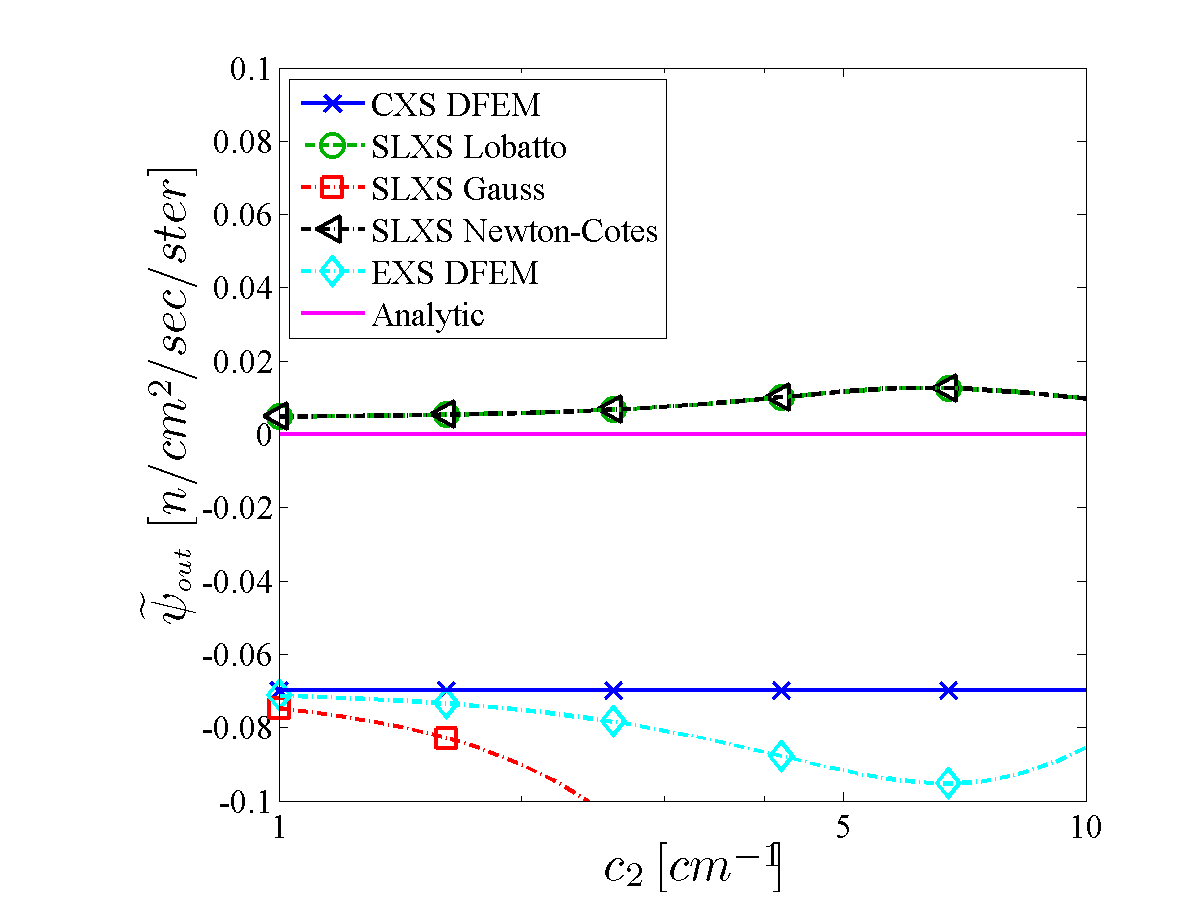
\includegraphics[width=11cm]{chapter3_variable_xs/Exp_outflow_p1.png}
}
\subfigure[Quadratic]{
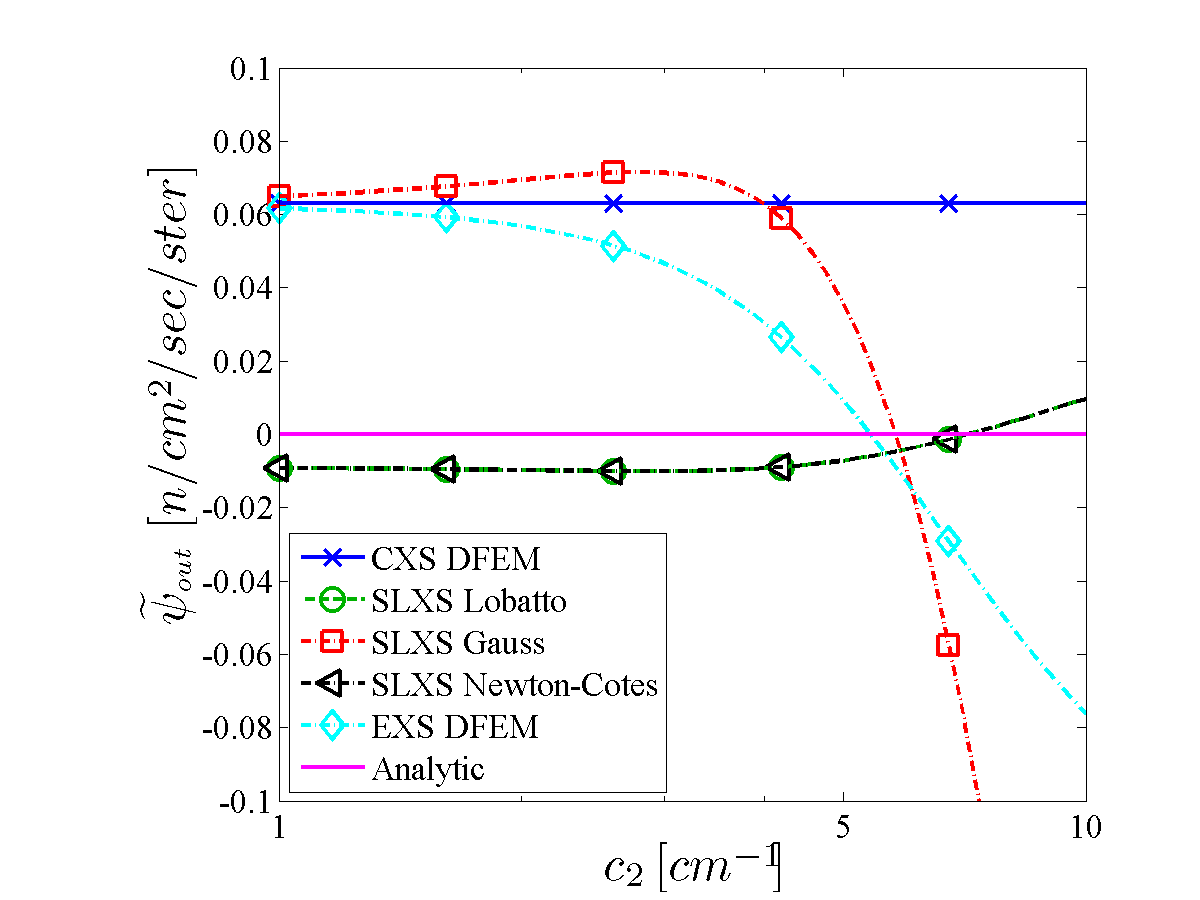
\includegraphics[width=11cm]{chapter3_variable_xs/Exp_outflow_p2.png}
}
\subfigure[Cubic]{
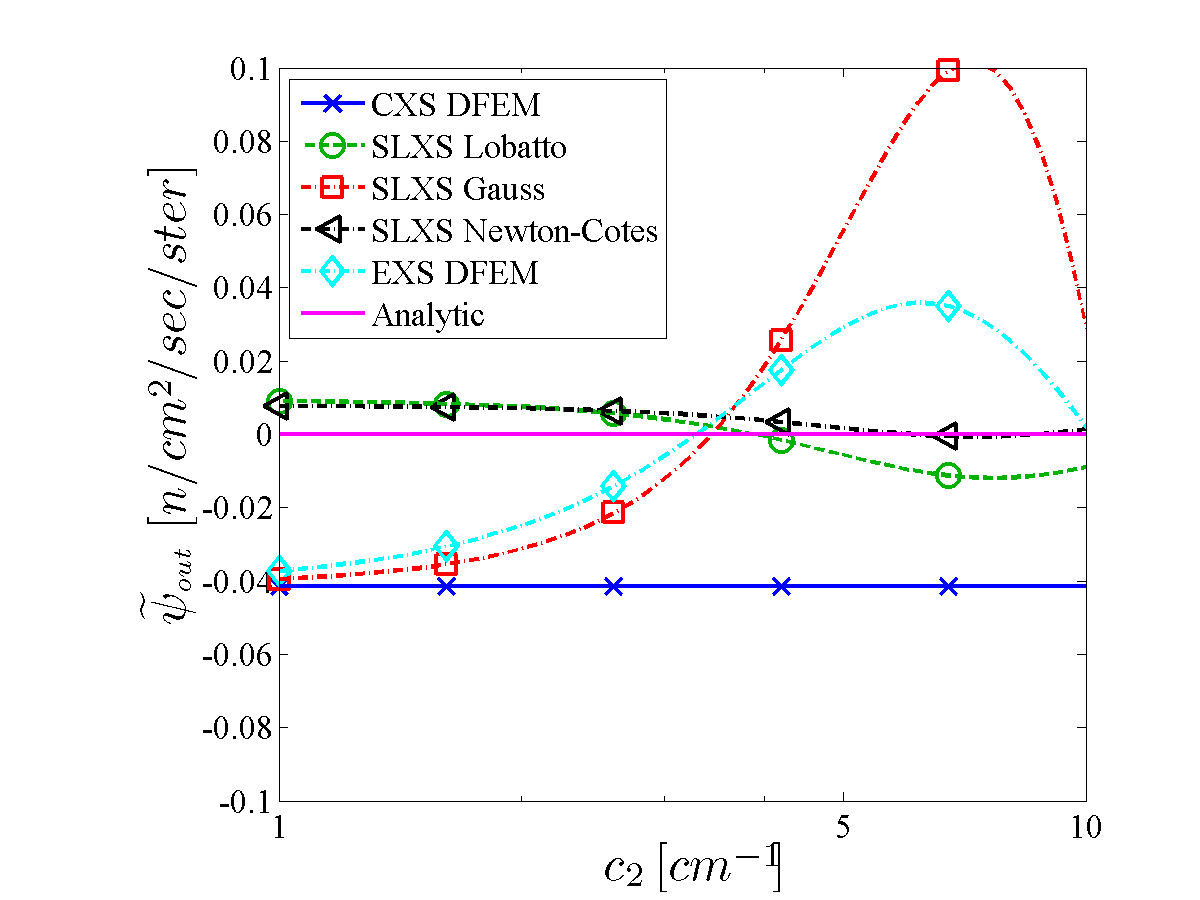
\includegraphics[width=11cm]{chapter3_variable_xs/Exp_outflow_p3.png}
}
\subfigure[4-th Order]{
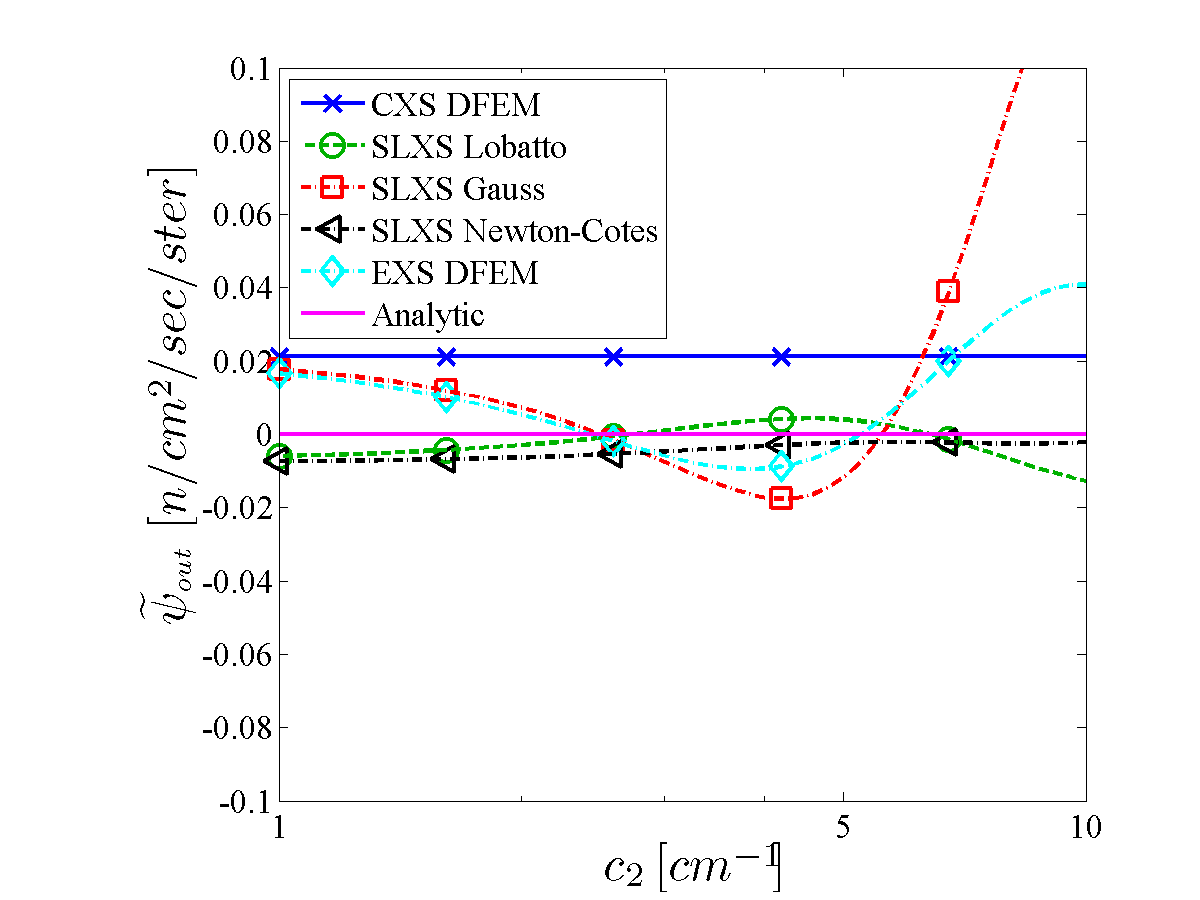
\includegraphics[width=11cm]{chapter3_variable_xs/Exp_outflow_p4.png}
}
\end{center}
\caption{Numerical outflow from single cell pure absorber with $\Sigma_t(x) = c_1e^{c_2 x}$, as a function of $c_2$ with constant optical thickness of twenty MFP, for different degree polynomial trial spaces.}
\label{fig:exp_outflow}
\end{figure}
We hold the total cell optical thickness to 20 mean-free-path (MFP), vary $c_2 \in [1,10]$, fix $x_R=1$, and $\mu_d =1$.
With an exponential cross section, the cell optical thickness in $MFP$ of a cell  with $x\in[0,x_R]$ is:
\benum
MFP = \int_{0}^{x_R}{\Sigma_t(x)~dx} = \frac{c_1}{c_2}\left( e^{c_2 x_R} - 1 \right) \pep
\label{eq:chap3_mfp_tot} 
\eenum
To maintain a constant optical thickness in \fig{fig:exp_outflow}, $c_1$ is required to be:
\benum
c_1 = \frac{c_2~MFP}{e^{c_2 x_R} - 1}\pep
\eenum
%In the results that follow, $x_R = 1$, $d_3 = \frac{MFP}{10 x_R}$, and $d_2$ is varied from $[0,10]$.  Results for a cell 1 MFP thick are given in \fig{fig:poly_xs_mfp_1}, for a cell 5 MFP thick in \fig{fig:poly_xs_mfp_5}, and for a cell 10 MFP thick in \fig{fig:poly_xs_mfp_10}.
%$d_1$ is adjusted to maintain the same number of MFP in each given plot.
%%  Arranging \eqt{eq:chap3_mfp_tot} $d_1$ will be defined as:
%%\benum
%%d_1 = \left(MFP - d_3 x_R \right)\frac{d_2+1}{x_R^{d_2+1}} \pep
%%\eenum
%Figures \ref{fig:poly_xs_mfp_1}-\ref{fig:poly_xs_mfp_10} show angular flux outflows as a function of trial space polynomial degree and $d_2$.  As $d_2$ is increased, the spatial variation of $\Sigma_t(x)$ increases.
%From Figs. \ref{fig:poly_xs_mfp_1}-\ref{fig:poly_xs_mfp_10} it is clear that total cell optical thickness alone does not regulate the positivity of angular flux outflow in a pure absorber with a spatially varying cross section.  
%
%
%The only methods that yield strictly positive angular flux outflow in our testing are CXS DFEM for even degree polynomial trial spaces, and 
%SLXS Lobatto and SLXS Newton-Cotes for the linear angular flux trial space.  
%
%
Figure \ref{fig:exp_outflow} confirms that  SLXS Lobatto (and the equivalent SLXS Newton-Cotes scheme) with a linear trial space is the only scheme that explicitly accounts for the spatial variation of cross and maintains a strictly positive angular flux outflow regardless of the shape of $\Sigma_t(x)$.
From \fig{fig:exp_outflow} we also observe that $\widetilde{\psi}_{out}$ varies for every method as a function of the shape of $\Sigma_t(x)$, with the obvious exception of CXS DFEM.
Considering that the analytic angular flux outflow is only a function of total cell MFP:
\benum
\label{eq:chap3_outflow_truth}
\psi_{out,i} = \psi_{in}(\mu_d) \exp\left[-\int_0^{x_{i+1/2}}{\Sigma_t(x)~dx}/ \mu_d \right] = \psi_{in}(\mu_d) \exp\left[-MFP~/\mu_d\right] \pec
\eenum
it is unphysical and undesirable that $\widetilde{\psi}_{out}$, for the SLXS Gauss, SLXS Lobatto, SLXS Newton-Cotes, and EXS DFEM schemes, depends on the spatial shape of $\Sigma_t(x)$.

%%%%%%%%%%%%%%%%%%%%%%%%%%%%%%%%%%%%%%%%%%%%%%%%%%%%%%%%%%%%%%%%%%%%%
\subsection{Multiple Cell Spatial Convergence Rates}
%%%%%%%%%%%%%%%%%%%%%%%%%%%%%%%%%%%%%%%%%%%%%%%%%%%%%%%%%%%%%%%%%%%%%

We now consider the order of spatial convergence for the following schemes: CXS DFEM, SLXS Gauss, SLXS Lobatto, and SLXS Newton-Cotes.  
Since exact integration of $\mathbf{R}_{\Sigma_t}$ is generally not feasible, we no longer consider the EXS DFEM scheme.  
Convergence results of the following angular flux errors as a function of the polynomial approximation order are presented:
\begin{subequations}
\beanum
E_{\psi} &=& \sqrt{\sum_{i=1}^{N_{cells}}{\int_{x_{i-1/2}}^{x_{i+1/2}}{ \left(\widetilde{\psi}_d(x) - \psi(x,\mu_d)  \right)^2  ~dx }}} \\
%E_{\psi_{in}} &=& \sqrt{\sum_{i=1}^{N_{cells}}{\Delta x_i\left(\widetilde{\psi}_{in,i} - \psi(x_{i-1/2})  \right)^2   }}  \\
E_{\psi_A} &=& \sqrt{\sum_{i=1}^{N_{cells}}{\Delta x_i\left(\widetilde{\psi}_{A,i} - \psi_{A,i}  \right)^2   }}  \\
E_{\psi_{out}} &=& \sqrt{\sum_{i=1}^{N_{cells}}{\Delta x_i\left(\widetilde{\psi}_{out,i} - \psi(x_{i+1/2},\mu_d)  \right)^2   }}  \pep
\eeanum
\label{eq:chap3_err_defs}
\end{subequations}
In \eqts{eq:chap3_err_defs}, $\Delta x_i$ is the width of cell $i$, cell $i$ spans $[x_{i-1/2},x_{i+1/2}]$, $\widetilde{\psi}_d(x)$ is the DFEM numerical approximation, $\psi(x,\mu_d)$ is the analytic solution (see \eqt{eq:chap3_exp_psi}).  The problem is spatially discretized using $N_{cells}$ spatial cells of equal width. 
We approximate the integrals defining the $L^2$ norm of the angular flux error, $E_{\psi}$, using a high-order Gauss quadrature set, $(w_{f,q},s_{f,q})$, with $N_{qf}$ points, such that:
\benum
\int_{x_{i-1/2}}^{x_{i+1/2}}{ \left(\widetilde{\psi}(x) - \psi(x,\mu_d)  \right)^2 ~dx}\approx 
\frac{\Delta x_i}{2}\sum_{q=1}^{N_{qf}}{ w_{f,q}\left( \widetilde{\psi}(s_{f,q}) - \psi(s_{f,q},\mu_d)\right)^2 }\pep
\eenum
For the results that follow, $N_{qf} = 10$.
We recall the definitions for the numerical approximations of the cell average angular flux, $\widetilde{\psi}_{A,i}$, and the outflow angular flux, $\widetilde{\psi}_{out,i}$:
\begin{subequations}
\beanum
%\widetilde{\psi}_{in,i} &=& \sum_{j=1}^{N_P}{\psi_{i,j} \B{j}(-1) } \\
\widetilde{\psi}_{A,i} &=& \frac{1}{2}\sum_{j=1}^{N_P}{w_j\psi_{i,j}  } \\
\widetilde{\psi}_{out,i} &=& \sum_{j=1}^{N_P}{\psi_{i,j} \B{j}(1) } \pep
\eeanum
\label{eq:chap3_num_defs}
\end{subequations}

We also consider the convergence of the numerical interaction rate, $\widetilde{IR}(x)$ to the true interaction rate $IR(x)$.  First, we define the analytic reaction rate for our beam problem:
\benum
IR(x) = \Sigma_t(x)\psi(x,\mu_d) \pep
\eenum
Similarly, we define a cell average interaction rate as:
\benum
IR_{A,i} = \frac{1}{\Delta x_i}\int_{x_{i-1/2}}^{x_{i+1/2}}{\Sigma_t(x)\psi(x,\mu_d)~dx} \pep
\eenum
%The numerical approximation to $IR(x)$ depends on the numerical scheme considered.  CXS DFEM is the simplest to consider.  Within cell $i$, CXS DFEM approximates $IR(x)$ as:
%\benum
%\widetilde{IR}(x) = \hat{\Sigma}_{t,i} \widetilde{\psi}(x,\mu_d) \pec
%\label{eq:chap3_cxs_I}
%\eenum
%with a cell average interaction rate approximated as:
%\benum
%\widetilde{IR}_{A,i} = \frac{\hat{\Sigma}_{t,i}}{2} \int_{-1}^1{ \widetilde{\psi}(s,\mu_d)~ds} = \hat{\Sigma}_{t,i} \widetilde{\psi}_{A,i}
%\eenum
Defining a point-wise numerical approximation, $\widetilde{IR}(x)$, to the analytic interaction rate for the self-lumping schemes presents a unique problem, since only a
a numerical quadrature is used to approximate the integrand of $\mathbf{R}$.  
Quadrature integration only requires point evaluations of $\Sigma_t(x)$, not knowledge of $\Sigma_t(x)$ in between quadrature points.
However, for the purpose of plotting the SLXS schemes, we define:
\benum
\widetilde{IR}(s) = \sum_{j=1}^{N_P}{\B{j}(s) \psi_{j,d} \Sigma_t(s_j) } \pep
\label{eq:chap3_sl_lump_inter}
\eenum

It must be emphasized that \eqt{eq:chap3_sl_lump_inter} is only used for plotting purposes.  
%For other purposes, such as calculating particle conservation, $L^2$ error estimates, etc., using the $\widetilde{IR}(s)$ given in \eqt{eq:chap3_sl_lump_inter} is either invalid or necessitates additional assumptions.
%such as assuming that $\Sigma_t(x)$ can be approximated as $\widetilde{\Sigma}_t(x)$:
%\benum
%\widetilde{\Sigma}_t(s) = \sum_{j=1}^{N_P}{\Sigma_t(s_j) \B{j}(s) } \pep
%%\eenum
%With respect to particle conservation, conservation statements must be evaluated with the same integration strategy used in forming the DFEM equations.  
%An easy way to show this is to consider the CXS DFEM scheme.
%Calculating the total absorption rate as:
%\benum
%\text{Total Absorptions}= \sum_{i=1}^{N_{cells}}{\frac{\Delta x_i}{2}\int_{-1}^1{\Sigma_t(s)\widetilde{\psi}(s,\mu_d) ~ds}} \pec
%\label{eq:chap3_abs_fake}
%\eenum
%using the true, spatially varying $\Sigma_t(s)$, will yield a different total absorption rate than using the cell average cross section method that was used to form the equations:
%\benum
%\text{Total Absorptions}= \sum_{i=1}^{N_{cells}}{\frac{\Delta x_i \hat{\Sigma}_{t,i}}{2}\int_{-1}^1{\widetilde{\psi}(s,\mu_d)~ds}} \pep
%\label{eq:chap3_conserve_cxs}
%\eenum
%%Results in a value of $\text{Total Absorption Rates}$ calculated by \eqt{eq:chap3_abs_fake} and \eqt{eq:chap3_conserve_cxs} are different.
%For \eqt{eq:chap3_abs_fake} and \eqt{eq:chap3_conserve_cxs} to be equivalent, $\Sigma_t(s)$ must be a constant, or $\hat{\Sigma}_{t,i}$ must calculated as in \eqt{eq:chap3_special}:
%\benum
%\label{eq:chap3_special}
%\hat{\Sigma}_{t,i} = \frac{\int_{-1}^1{ \Sigma_t(s) \widetilde{\psi}(s,\mu_d)~ds }}{\int_{-1}^1{\widetilde{\psi}(s,\mu_d)~ds}} \pep
%\eenum
%However, calculating $\hat{\Sigma}_{t,i}$ as in \eqt{eq:chap3_special} requires the transport solution to be known first, or requires a non-linear solution process.
We approximate the cell average interaction rate in cell $i$ as:
\benum
\label{eq:chap3_ia_calc}
\widetilde{IR}_{A,i} = \frac{1}{2}\sum_{j=1}^{N_P}{w_j \Sigma_t(s_j) \psi_{j,d} }\pep
\eenum
In \eqt{eq:chap3_ia_calc}, $\Sigma_t(s_j) = \hat{\Sigma}_t$ for the CXS DFEM scheme, and $\Sigma_t(s_j)$ is the point evaluation of the true cross section for all other schemes.

We consider two measures to assess the error of the DFEM schemes' approximation of the true interaction rate, $IR(x)$.  The first, $E_{IR}$ is an approximation of the $L^2$ norm of interaction rate error:
\benum
E_{IR} = \sqrt{
\sum_{i=1}^{N_{cells}}{\frac{\Delta x_i}{2} \sum_{q=1}^{N_P}{w_q \left( IR(s_q) - \Sigma_t(s_q)\widetilde{\psi}(s_q,\mu_d) \right)^2}}
} \pep
\label{eq:chap3_EIR}
\eenum
We reiterate that, for the self-lumping schemes, $\widetilde{IR}(s)$ is only truly defined at the DFEM interpolation points.
%Although less accurate than using a fine quadrature, we evaluate \eqt{eq:chap3_EIR} with quadrature restricted to the DFEM interpolation points, since the self-lumping schemes only conserve particles if $\widetilde{IR}(s)$ is evaluated at the angular flux DFEM interpolation points.
$E_{IR_A}$ measures the convergence of the average interaction rate:
\benum
E_{IR_A} = \sqrt{\sum_{i=1}^{N_{cells}}{\Delta x_i (IR_{A,i} - \widetilde{IR}_{A,i})^2}} \pep
\eenum

For our convergence study, we consider a source-free purely absorbing slab with a cross section that varies exponentially in space as in \eqt{eq:chap3_xs_form} with $c_1 = 0.1$ and $c_2 = 2\ln(10)$.  
A beam of radiation is incident on the left face in the direction of $\mu_d=1$, vacuum boundary conditions exist on the right face of the slab, and $x\in[0, 1]$.  
The convergence of the $E_{\psi}$,  $E_{\psi_A}$, and $E_{\psi_{out}}$ as a function of the choice of numerical scheme and trial space polynomial degree are given in \fig{fig:varxs_psi_L2},  \fig{fig:varxs_psi_A}, and \fig{fig:varxs_psi_out}, respectively.  
\begin{figure}[!htp]
\begin{center}
\subfigure[Linear]{
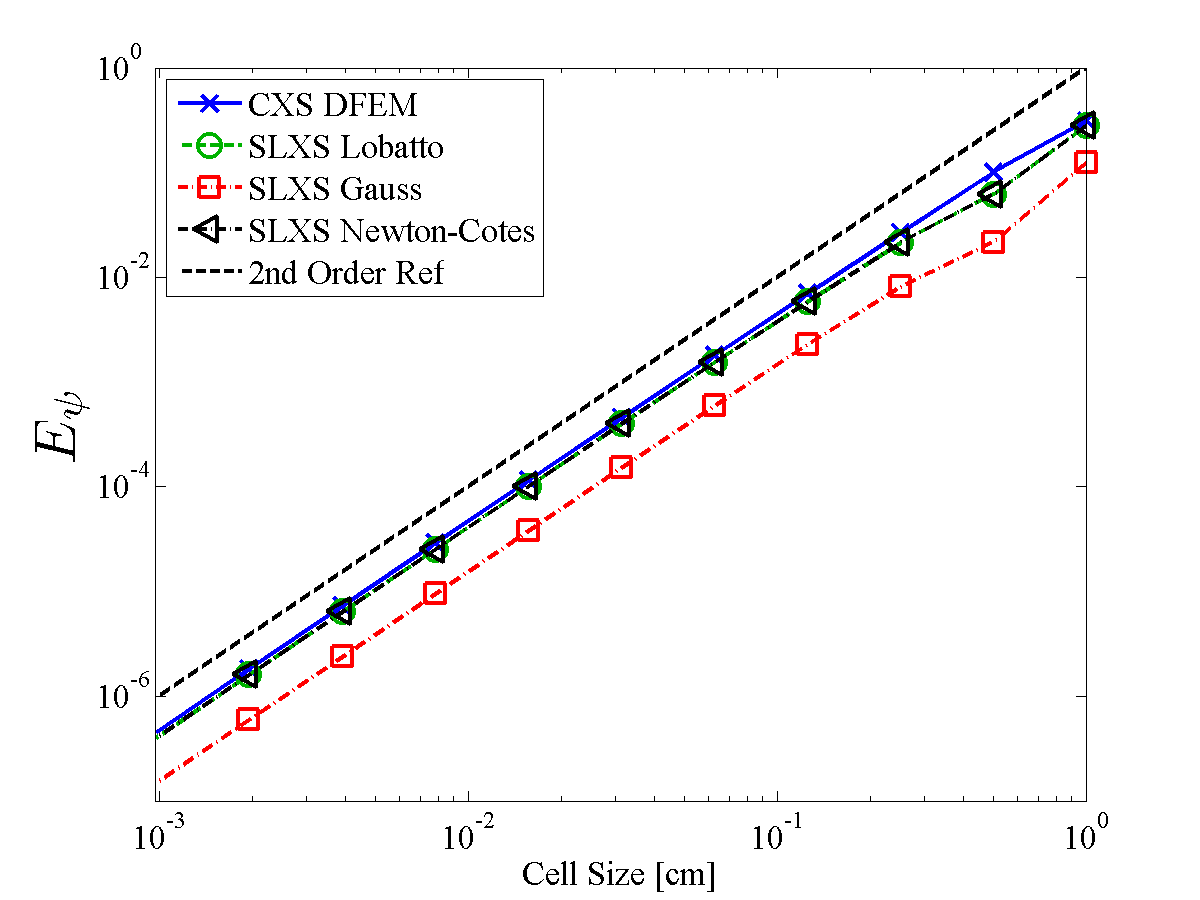
\includegraphics[width=11cm]{chapter3_variable_xs/P1_VarXS_E_psi_L2.png}
}
\subfigure[Quadratic]{
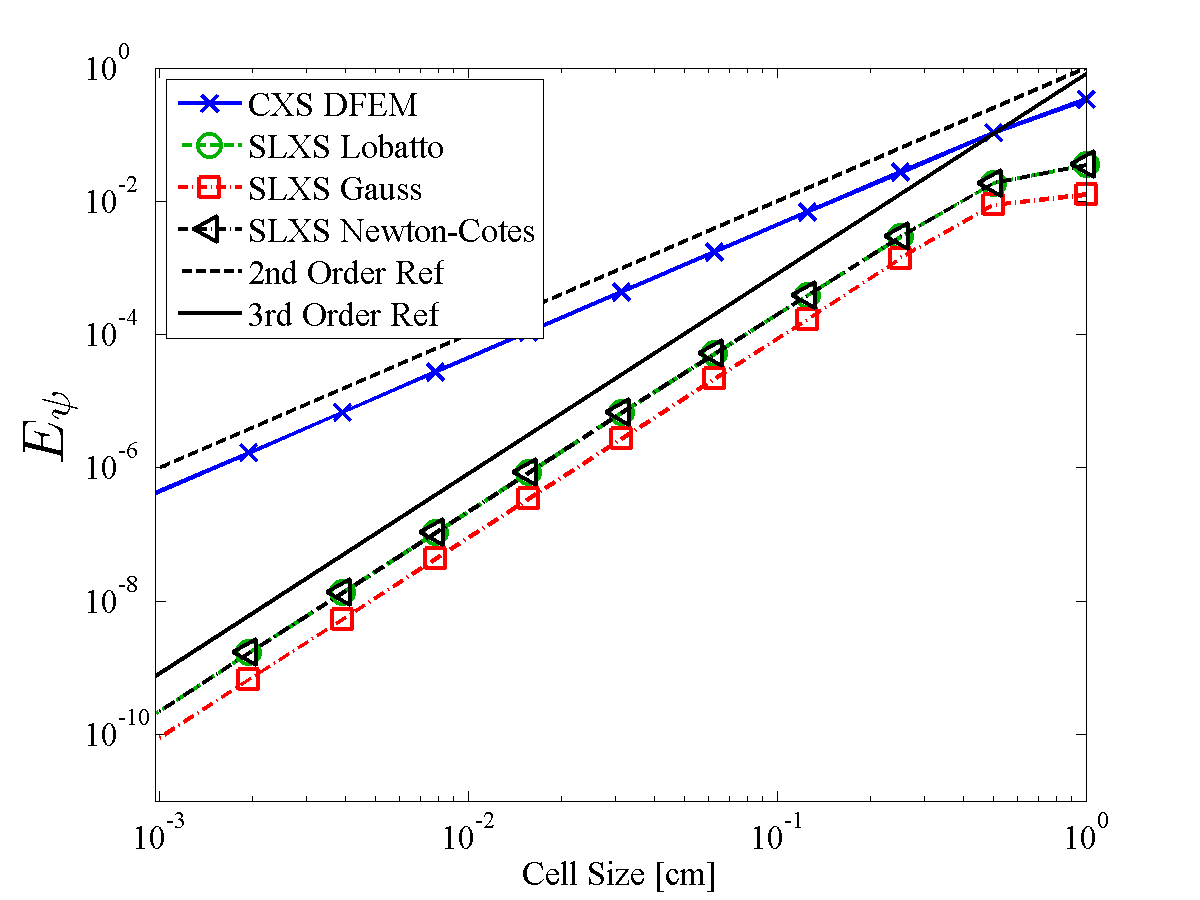
\includegraphics[width=11cm]{chapter3_variable_xs/P2_VarXS_E_psi_L2.png}
}
\subfigure[Cubic]{
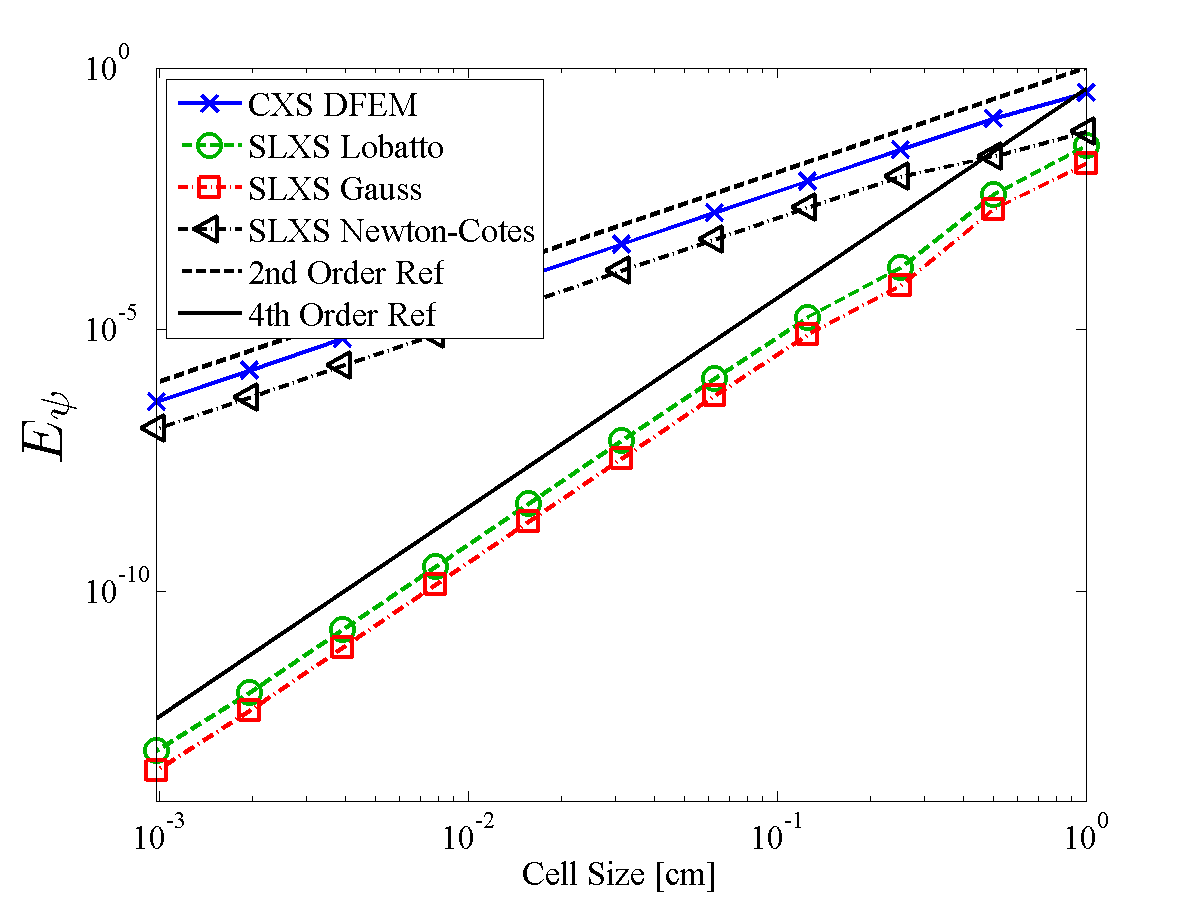
\includegraphics[width=11cm]{chapter3_variable_xs/P3_VarXS_E_psi_L2.png}
}
\subfigure[4-th Order]{
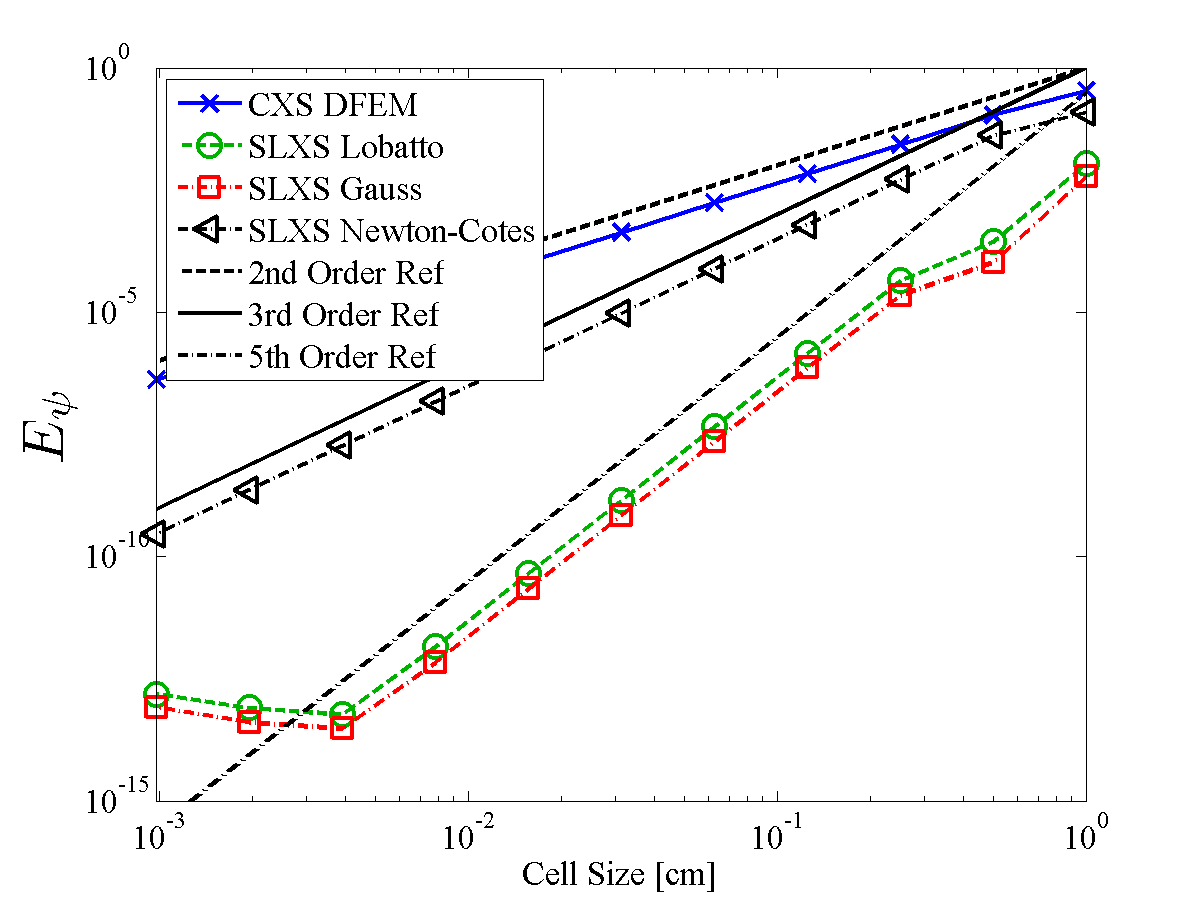
\includegraphics[width=11cm]{chapter3_variable_xs/P4_VarXS_E_psi_L2.png}
}
\end{center}
\caption{Convergence of $E_{\psi}$ for a multiple cell problem as a function of cell size for a pure absorber with exponentially varying cross section, $c_1 = 0.1~[cm^{-1}]$, $c_2 = 2\ln(10)~[cm^{-1}]$, and $x\in \left[0,1~[cm] \right]$.}
\label{fig:varxs_psi_L2}
\end{figure}
%
%
%
\begin{figure}[!htp]
\begin{center}
\subfigure[Linear]{
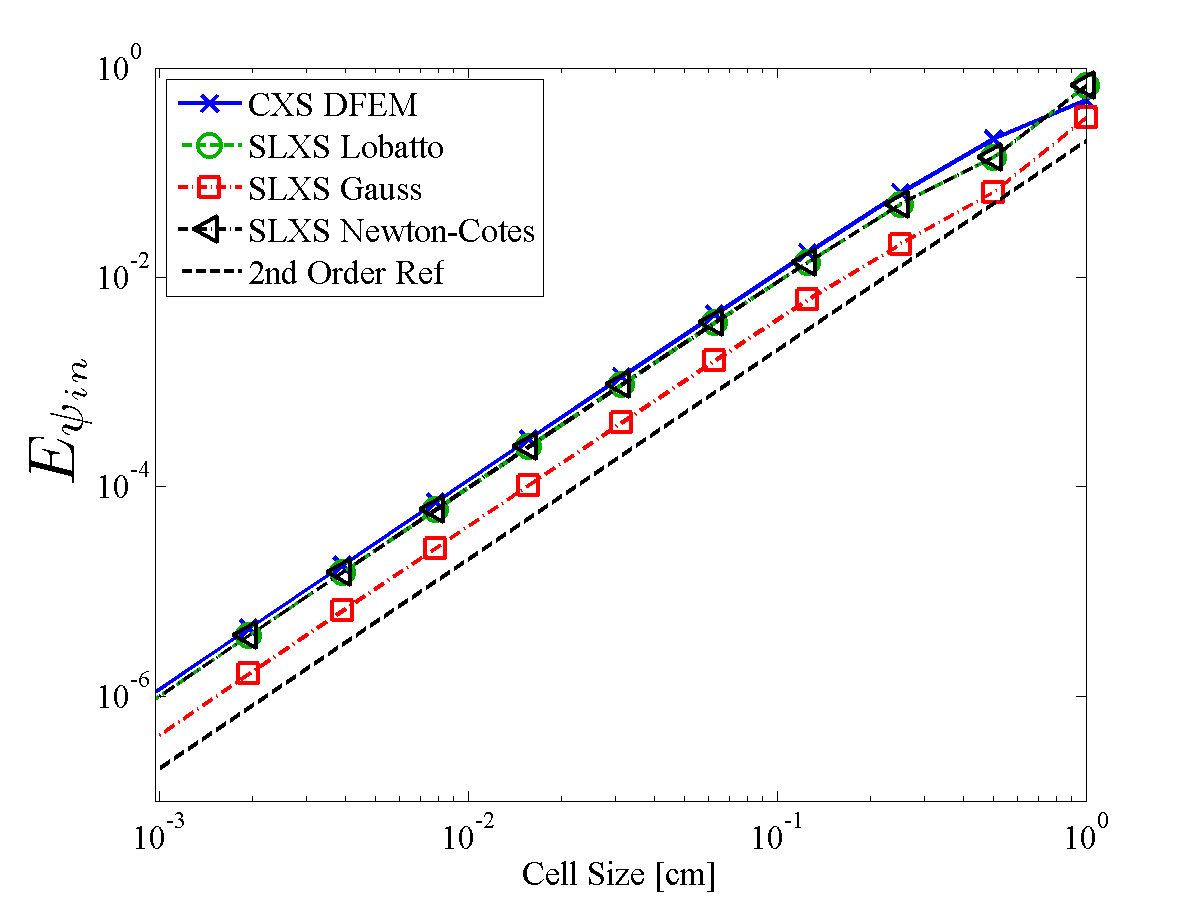
\includegraphics[width=11cm]{chapter3_variable_xs/P1_VarXS_E_psi_in.png}
}
\subfigure[Quadratic]{
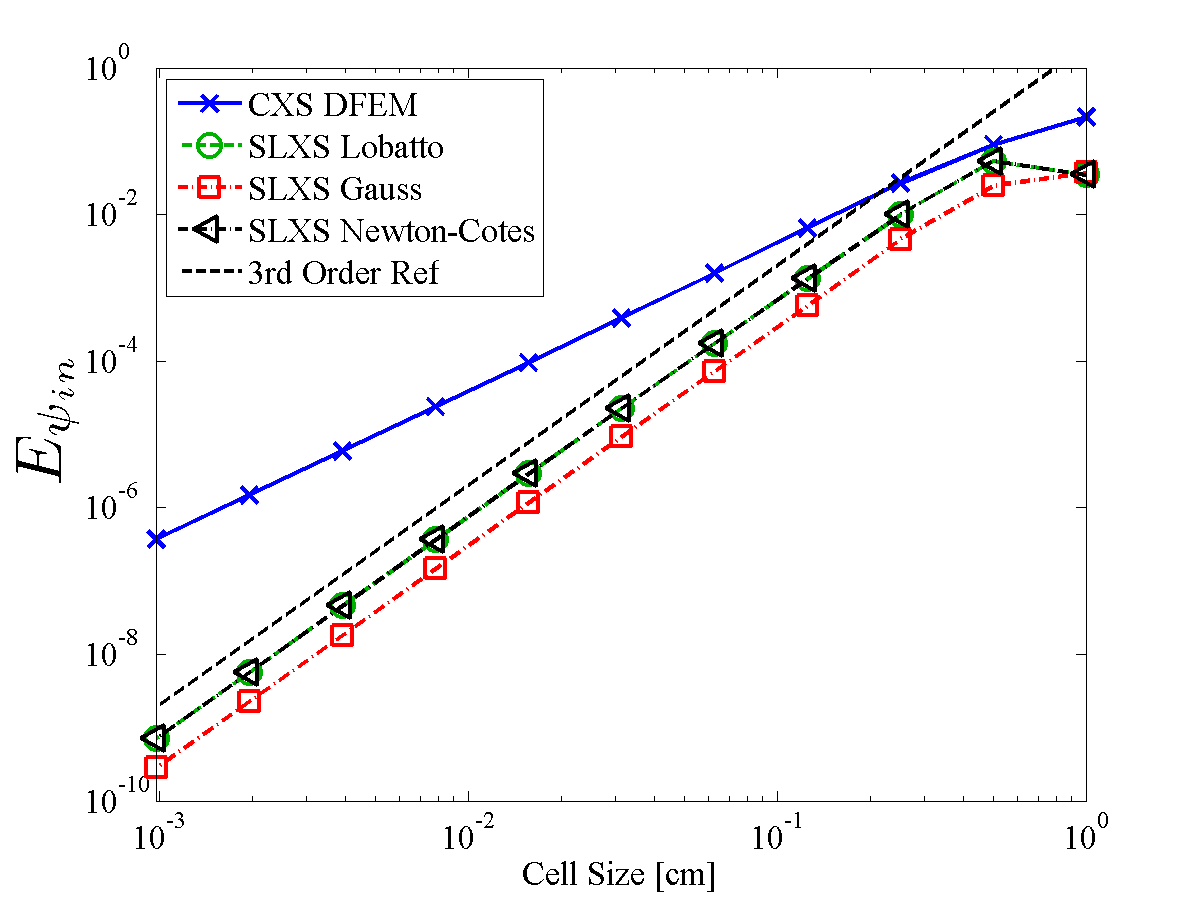
\includegraphics[width=11cm]{chapter3_variable_xs/P2_VarXS_E_psi_in.png}
}
\subfigure[Cubic]{
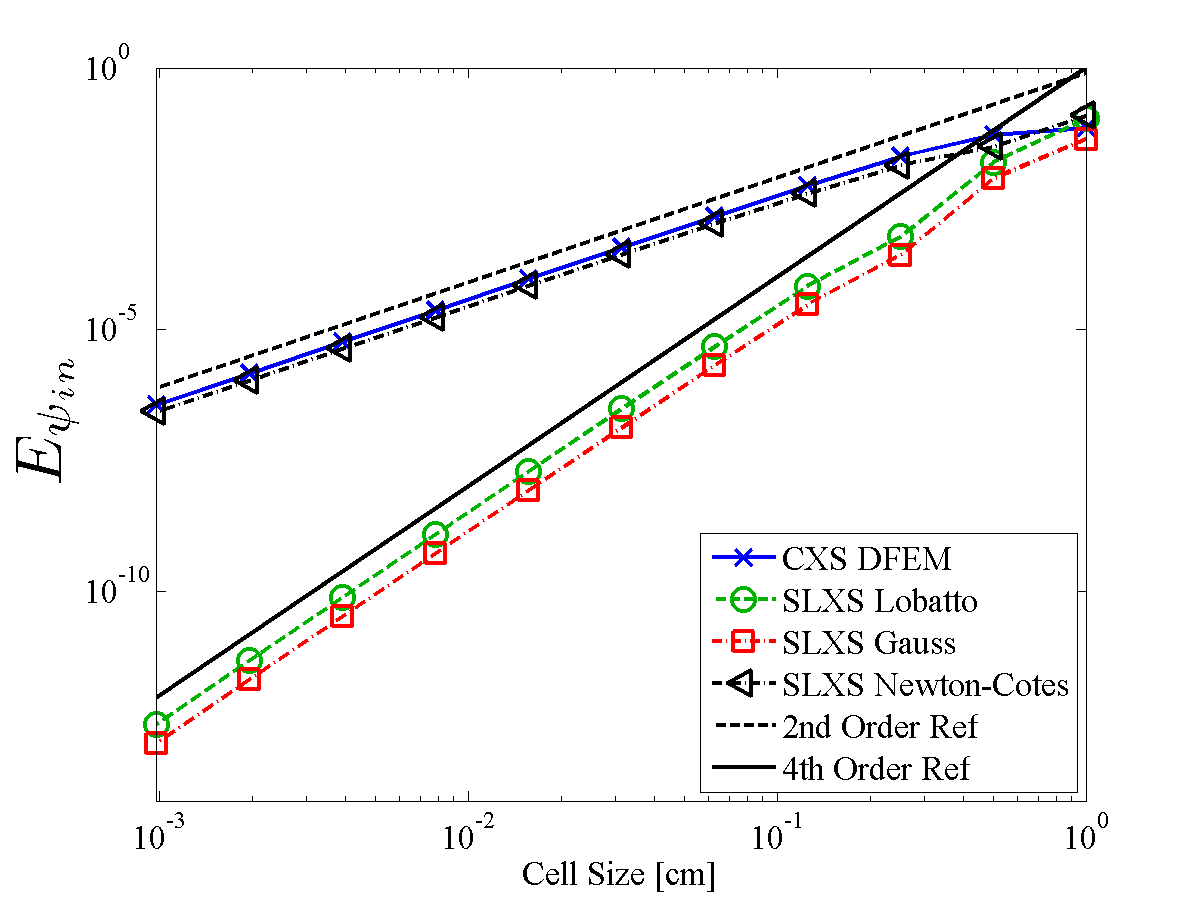
\includegraphics[width=11cm]{chapter3_variable_xs/P3_VarXS_E_psi_in.png}
}
\subfigure[4-th Order]{
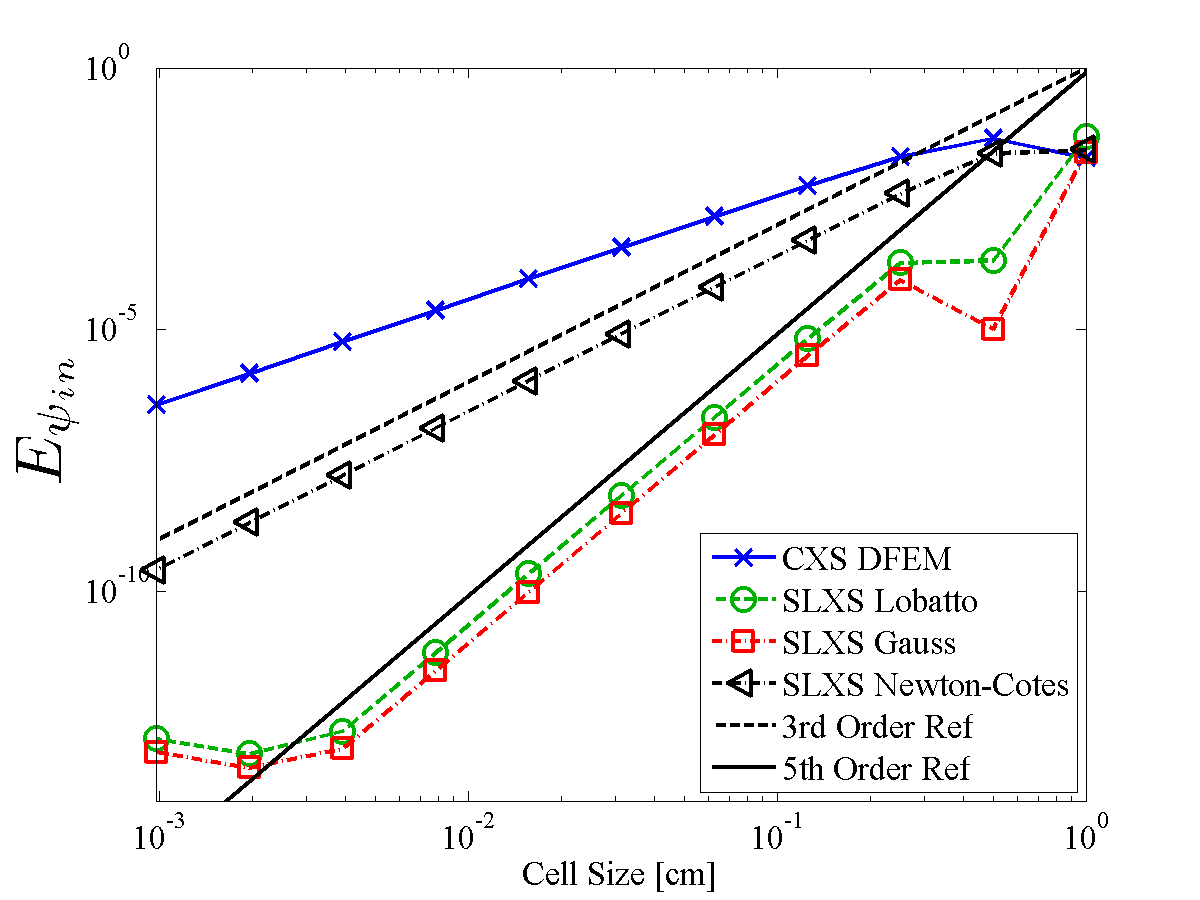
\includegraphics[width=11cm]{chapter3_variable_xs/P4_VarXS_E_psi_in.png}
}
\end{center}
\caption{Convergence of $E_{\psi_{in}}$ for a multiple cell problem as a function of cell size for a pure absorber with exponentially varying cross section, $c_3=10$, $c_1 = 0.1~[cm^{-1}]$, $c_2 = 2~[cm^{-1}]$, and $x\in \left[0,1~[cm] \right]$.}
\label{fig:varxs_psi_in}
\end{figure}
%
%
%
\begin{figure}[!htp]
\begin{center}
\subfigure[Linear]{
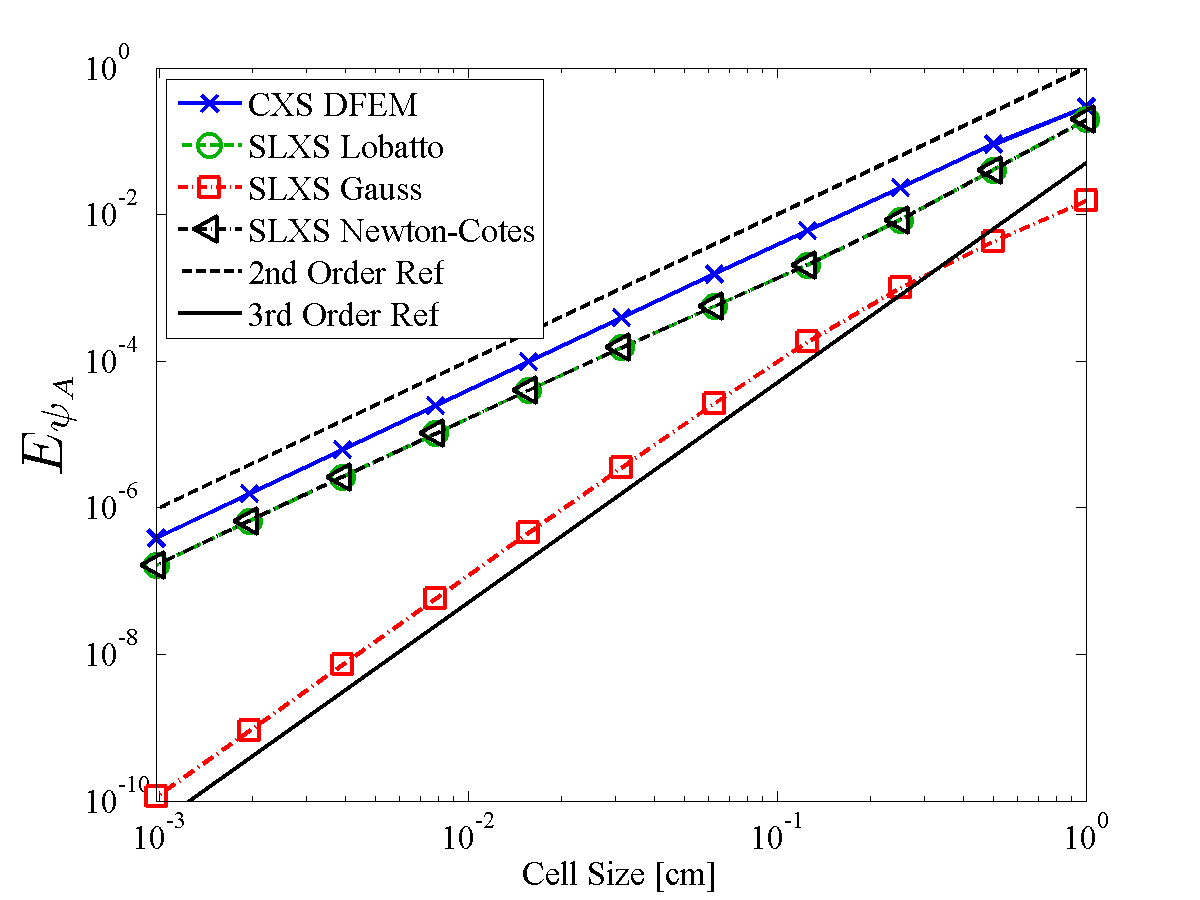
\includegraphics[width=11cm]{chapter3_variable_xs/P1_VarXS_E_psi_A.png}
}
\subfigure[Quadratic]{
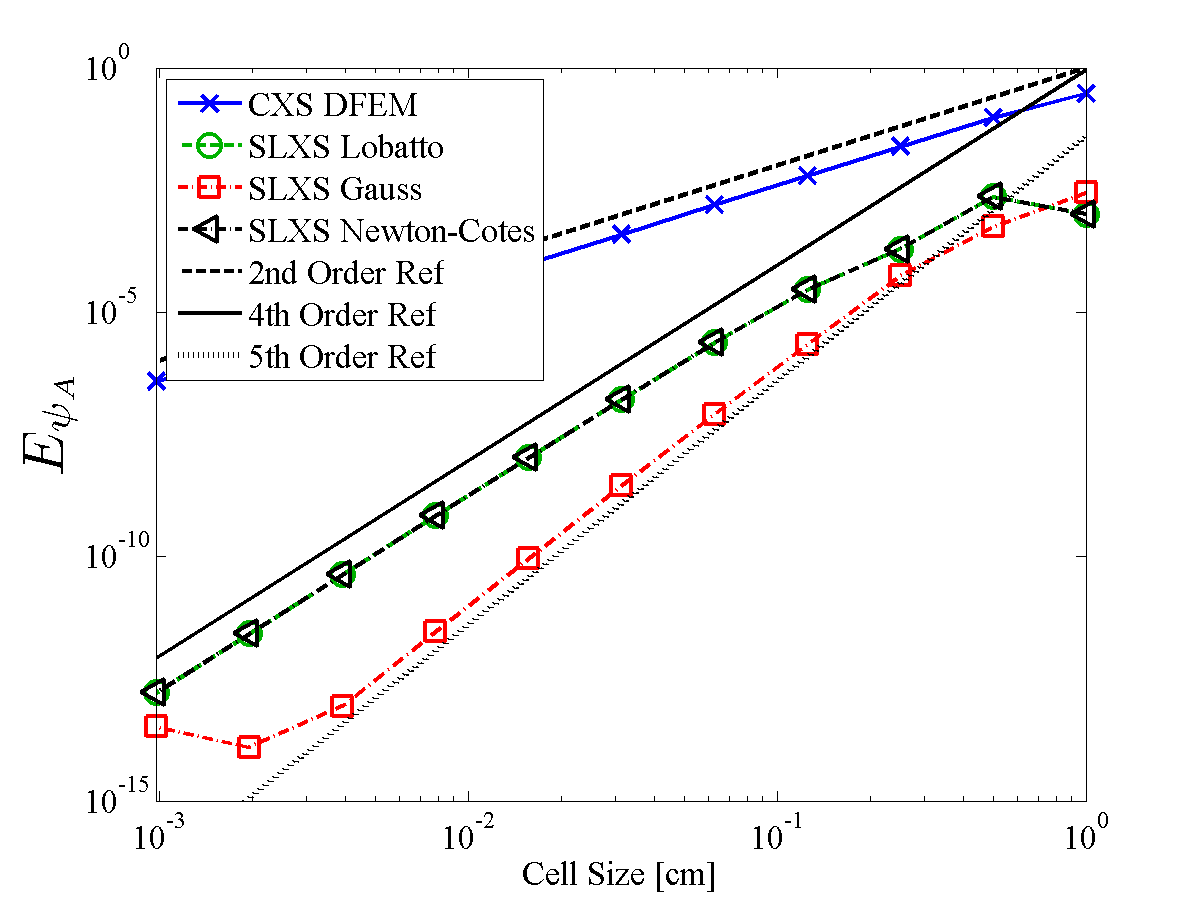
\includegraphics[width=11cm]{chapter3_variable_xs/P2_VarXS_E_psi_A.png}
}
\subfigure[Cubic]{
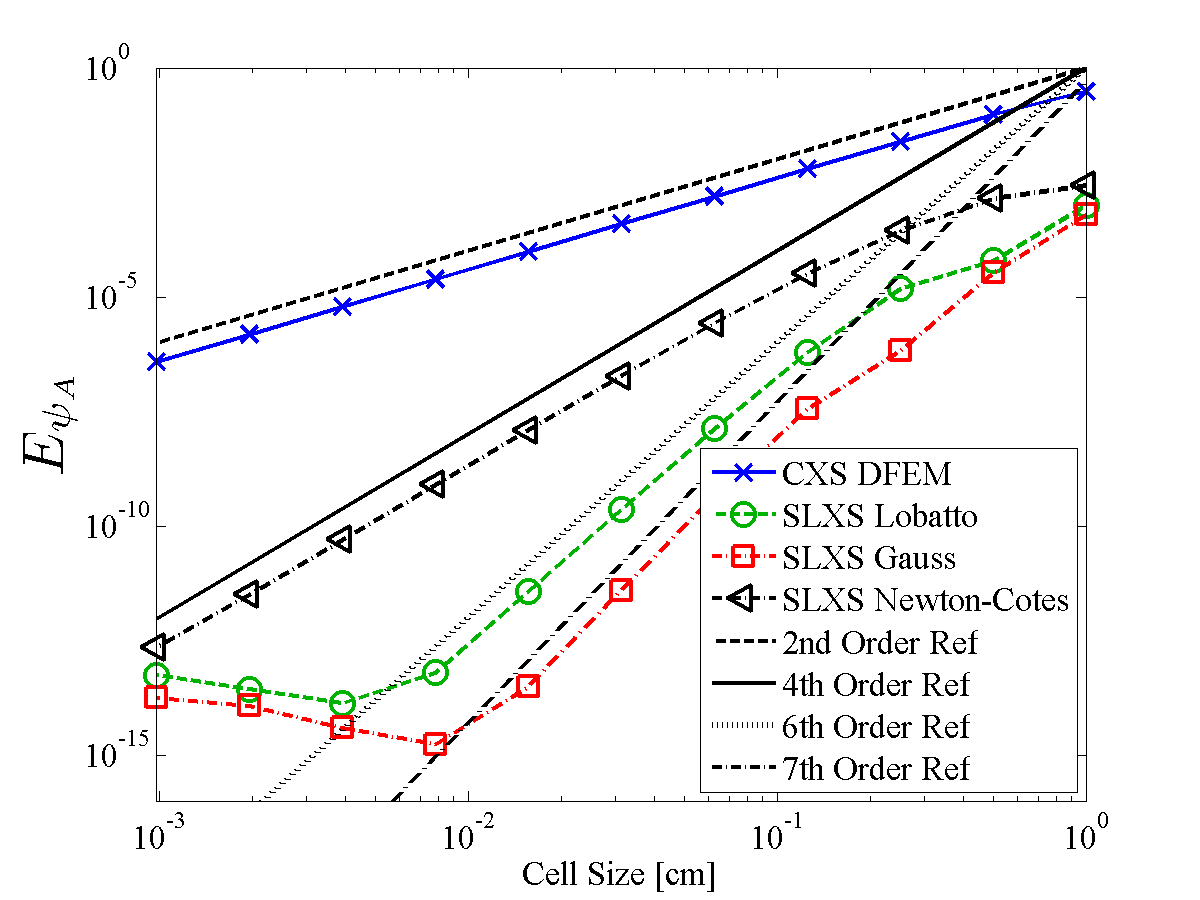
\includegraphics[width=11cm]{chapter3_variable_xs/P3_VarXS_E_psi_A.png}
}
\subfigure[4-th Order]{
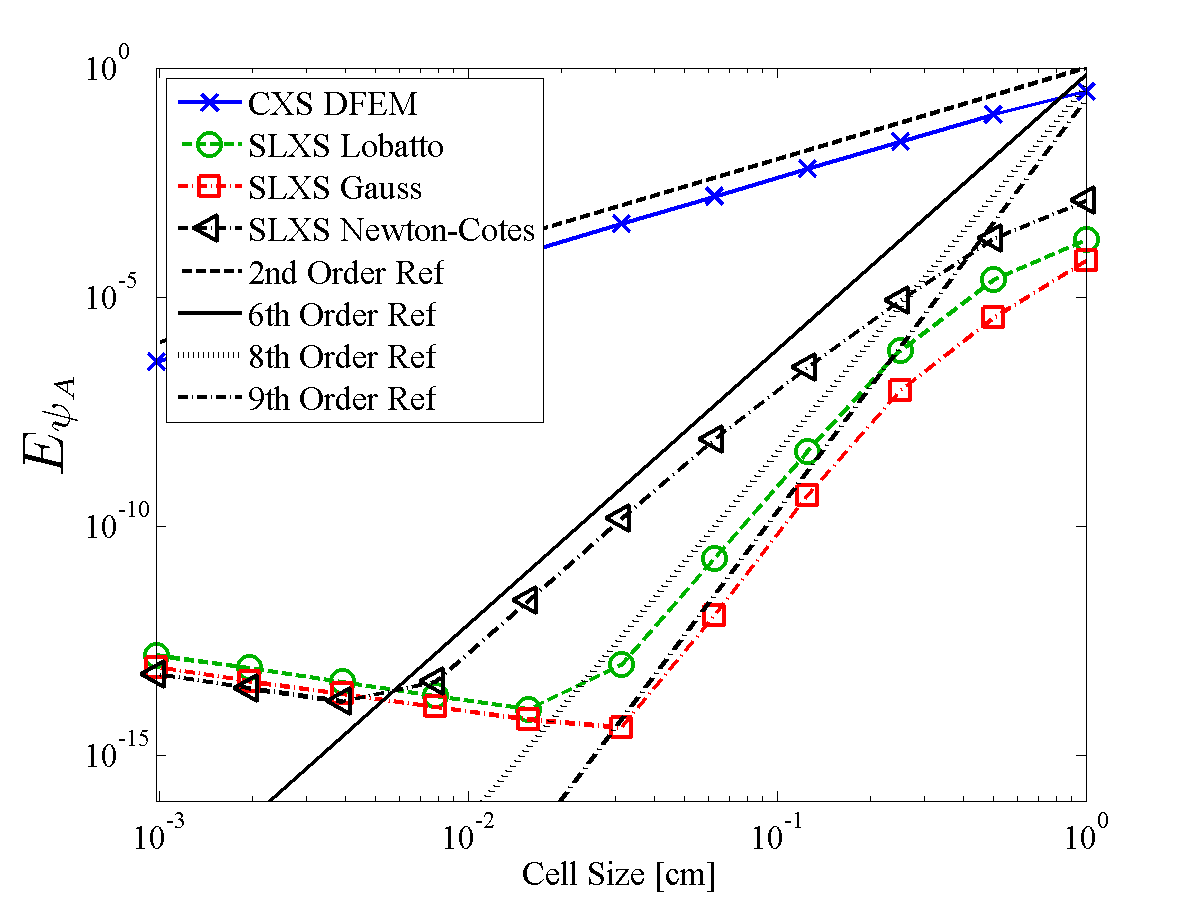
\includegraphics[width=11cm]{chapter3_variable_xs/P4_VarXS_E_psi_A.png}
}
\end{center}
\caption{Convergence of $E_{\psi_A}$ for a multiple cell problem as a function of cell size for a pure absorber with exponentially varying cross section, $c_1 = 0.1~[cm^{-1}]$, $c_2 = 2\ln(10)~[cm^{-1}]$, and $x\in \left[0,1~[cm] \right]$.}
\label{fig:varxs_psi_A}
\end{figure}
%
%
%
\begin{figure}[!htp]
\begin{center}
\subfigure[Linear]{
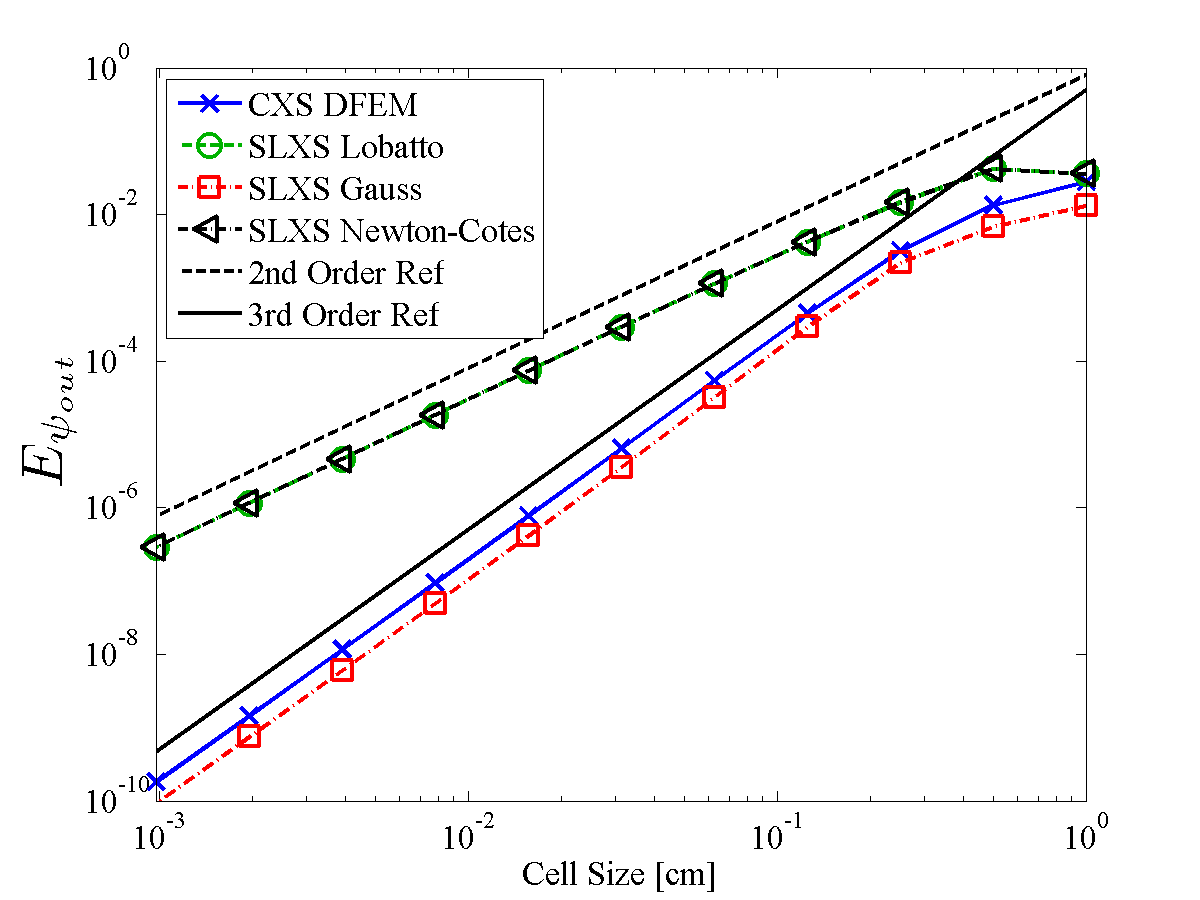
\includegraphics[width=11cm]{chapter3_variable_xs/P1_VarXS_E_psi_out.png}
}
\subfigure[Quadratic]{
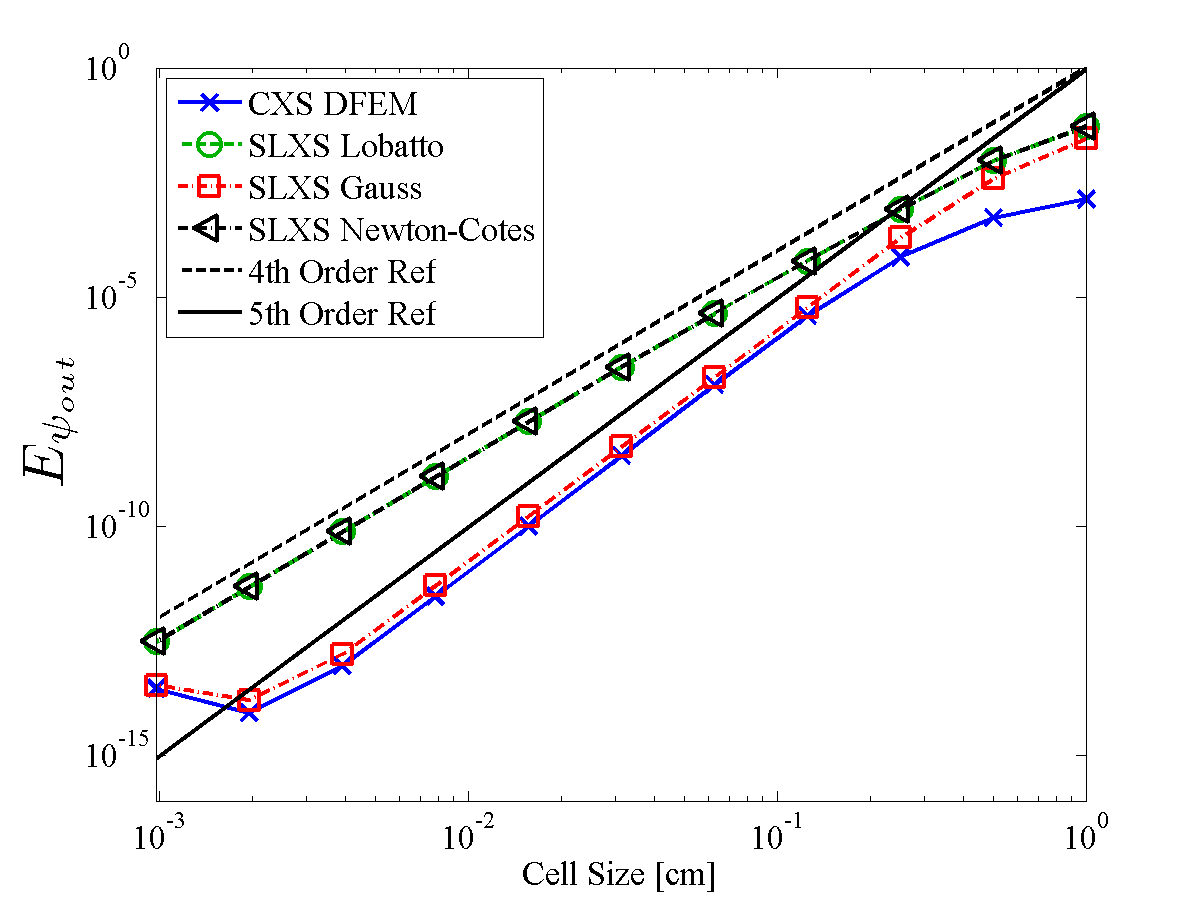
\includegraphics[width=11cm]{chapter3_variable_xs/P2_VarXS_E_psi_out.png}
}
\subfigure[Cubic]{
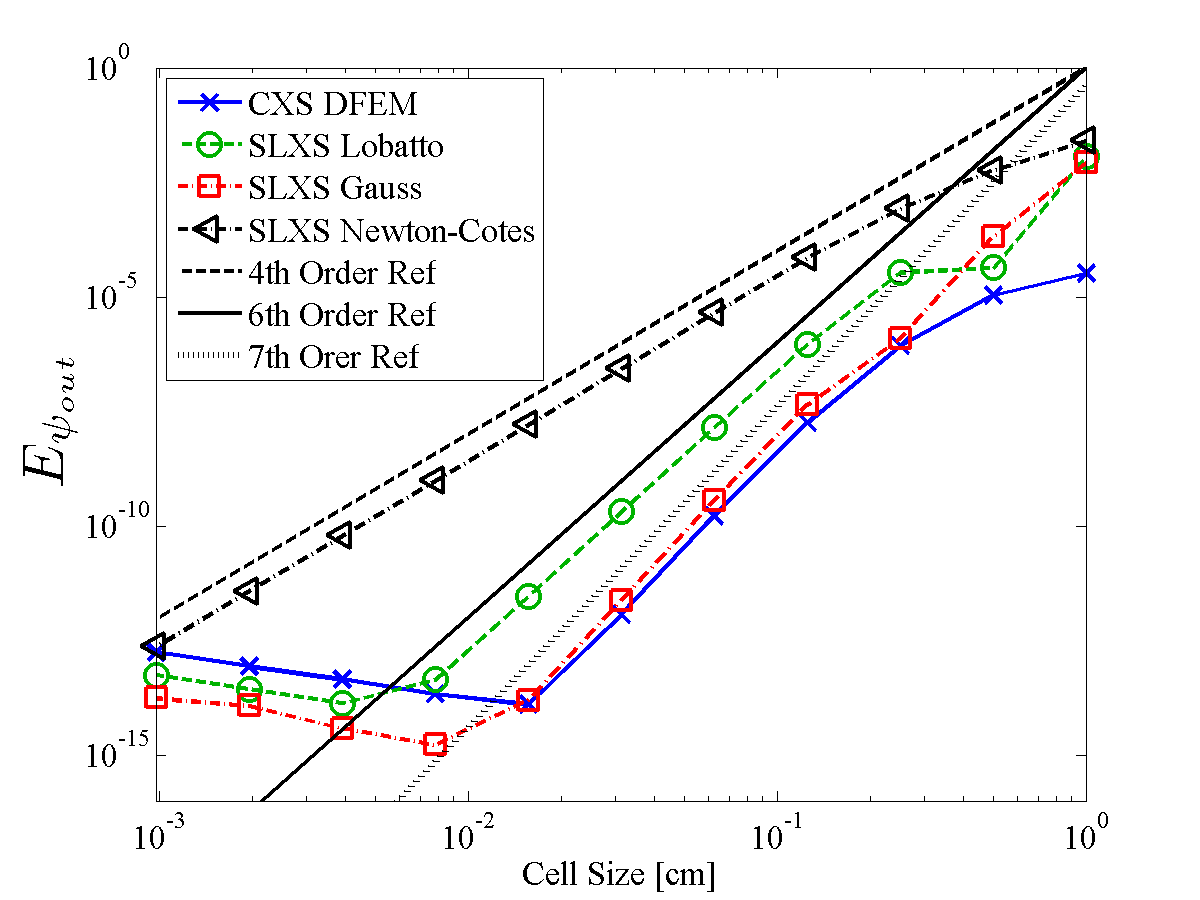
\includegraphics[width=11cm]{chapter3_variable_xs/P3_VarXS_E_psi_out.png}
}
\subfigure[4-th Order]{
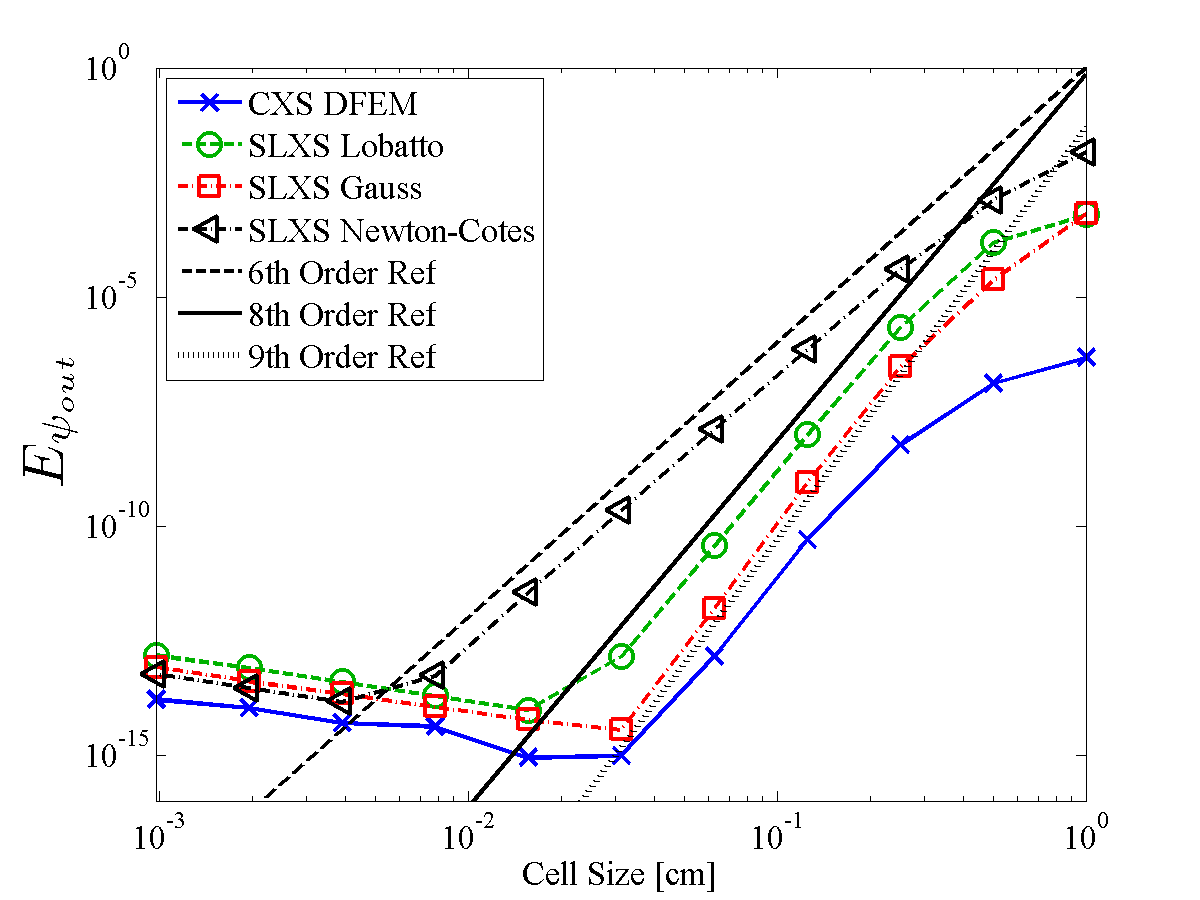
\includegraphics[width=11cm]{chapter3_variable_xs/P4_VarXS_E_psi_out.png}
}
\end{center}
\caption{Convergence of $E_{\psi_{out}}$ for a multiple cell problem as a function of cell size for a pure absorber with exponentially varying cross section, $c_1 = 0.1~[cm^{-1}]$, $c_2 = 2\ln(10)~[cm^{-1}]$, and $x\in \left[0,1~[cm] \right]$.}
\label{fig:varxs_psi_out}
\end{figure}
%
%
Convergence of $E_{IR}$ and $E_{IR_A}$ as function of numerical scheme and trial space polynomial degree are given in \fig{fig:varxs_I_L2} and \fig{fig:varxs_I_A}. 
%
%
\begin{figure}[!htp]
\begin{center}
\subfigure[Linear]{
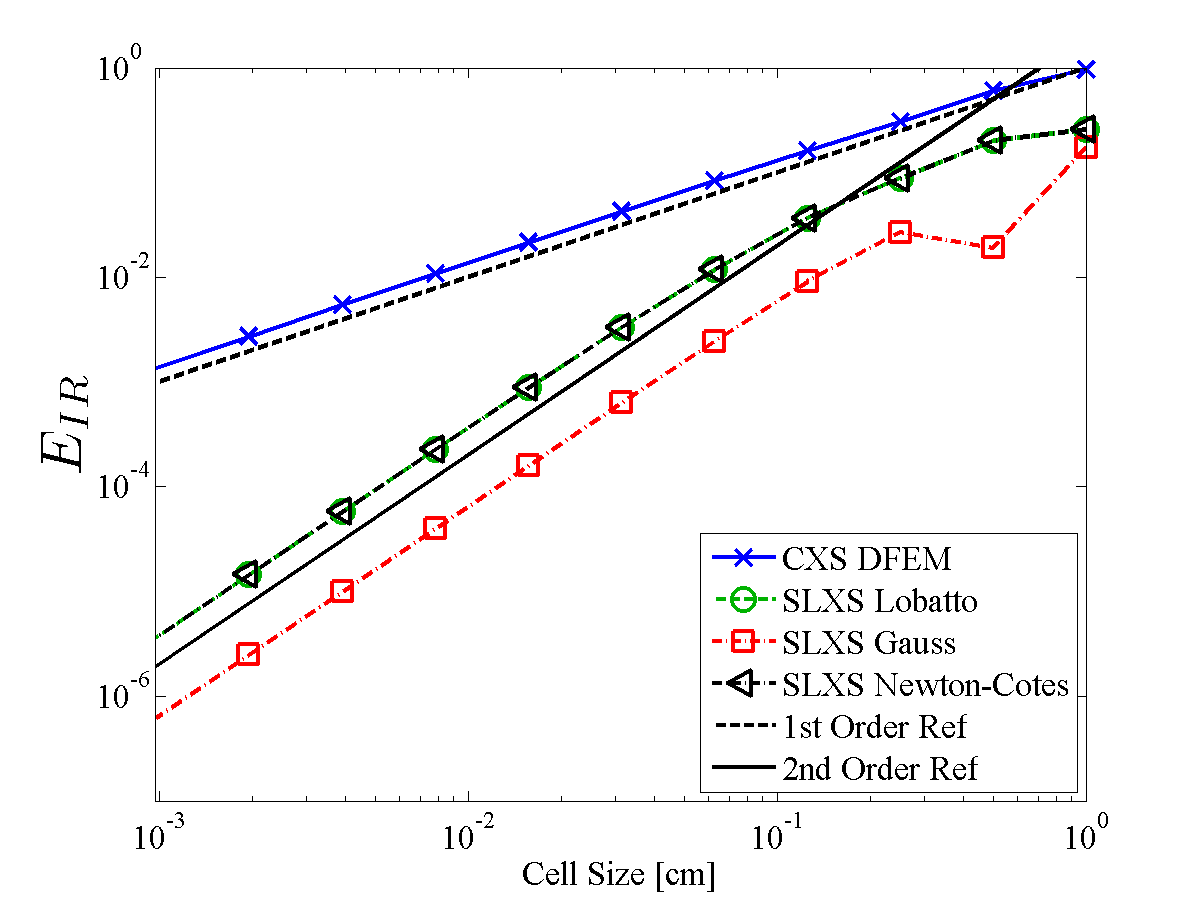
\includegraphics[width=11cm]{chapter3_variable_xs/P1_VarXS_E_I_L2.png}
}
\subfigure[Quadratic]{
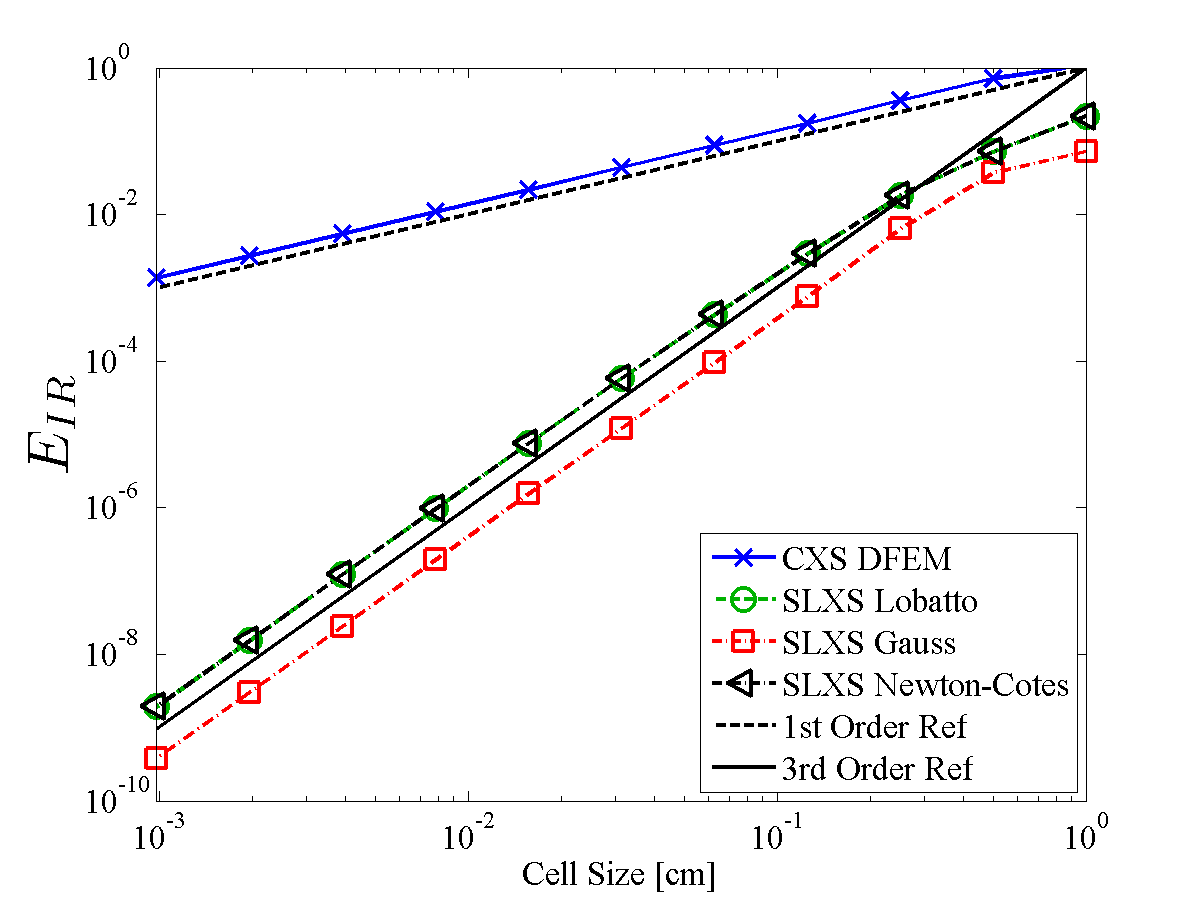
\includegraphics[width=11cm]{chapter3_variable_xs/P2_VarXS_E_I_L2.png}
}
\subfigure[Cubic]{
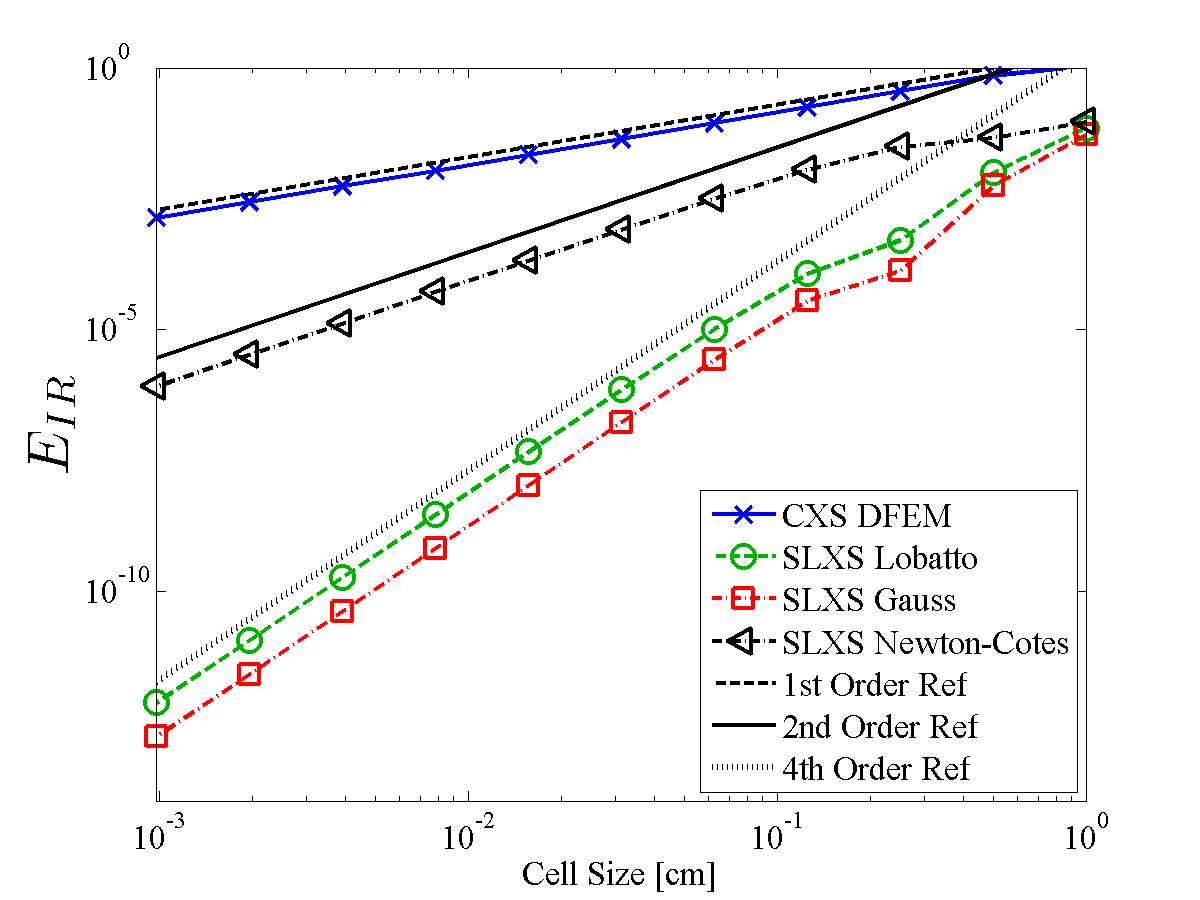
\includegraphics[width=11cm]{chapter3_variable_xs/P3_VarXS_E_I_L2.png}
}
\subfigure[4-th Order]{
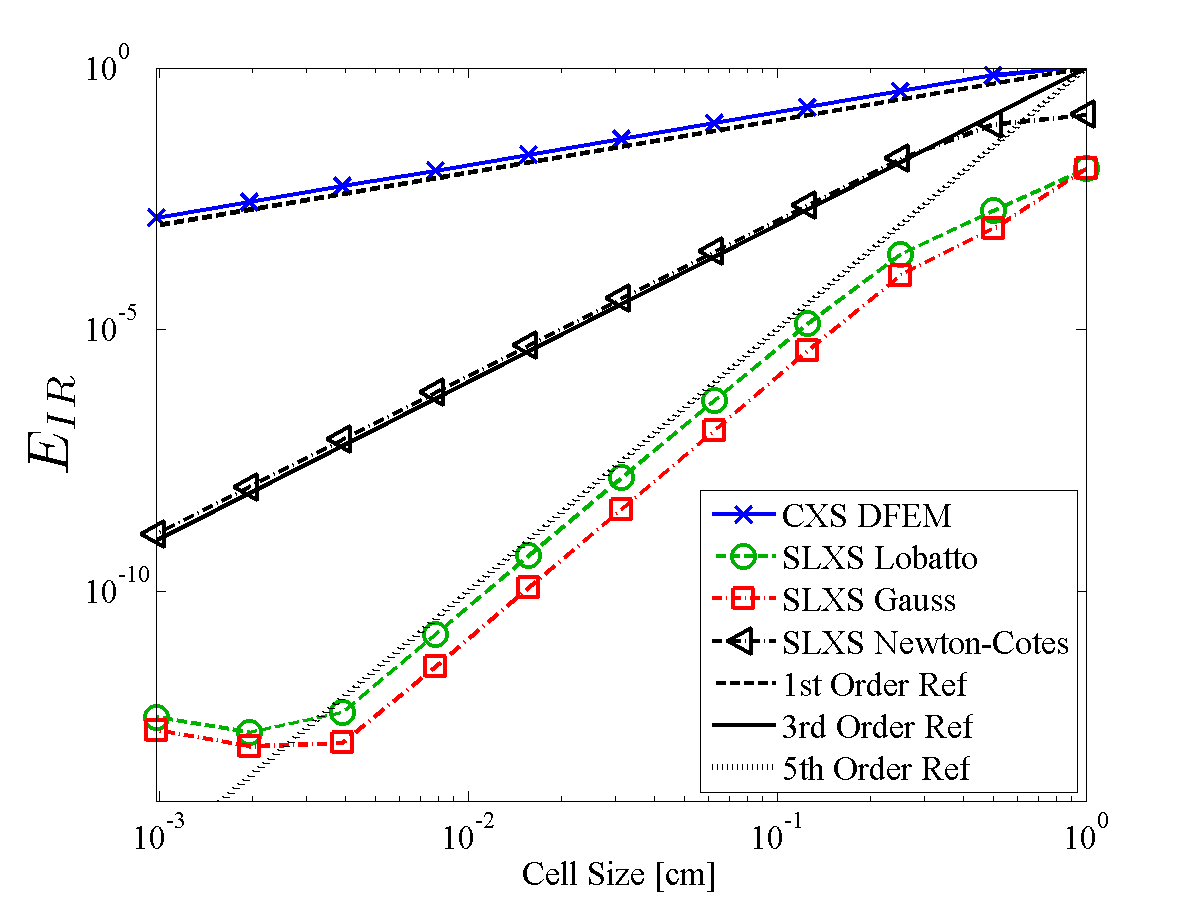
\includegraphics[width=11cm]{chapter3_variable_xs/P4_VarXS_E_I_L2.png}
}
\end{center}
\caption{Convergence of $E_{IR}$ for a multiple cell problem as a function of cell size for a pure absorber with exponentially varying cross section, $c_1 = 0.1~[cm^{-1}]$, $c_2 = 2\ln(10)~[cm^{-1}]$, and $x\in \left[0,1~[cm] \right]$.}
\label{fig:varxs_I_L2}
\end{figure}
%
%
%
\begin{figure}[!htp]
\begin{center}
\subfigure[Linear]{
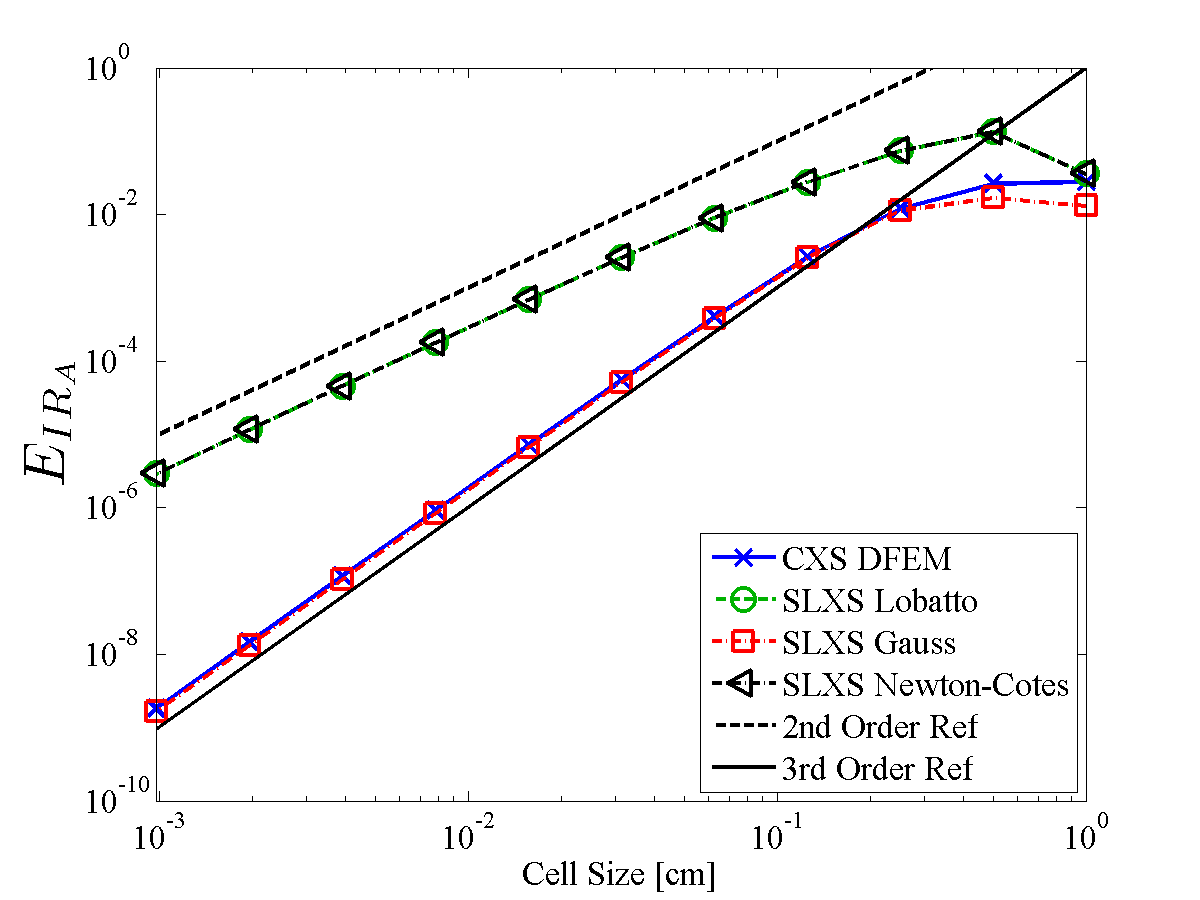
\includegraphics[width=11cm]{chapter3_variable_xs/P1_VarXS_E_I_A.png}
}
\subfigure[Quadratic]{
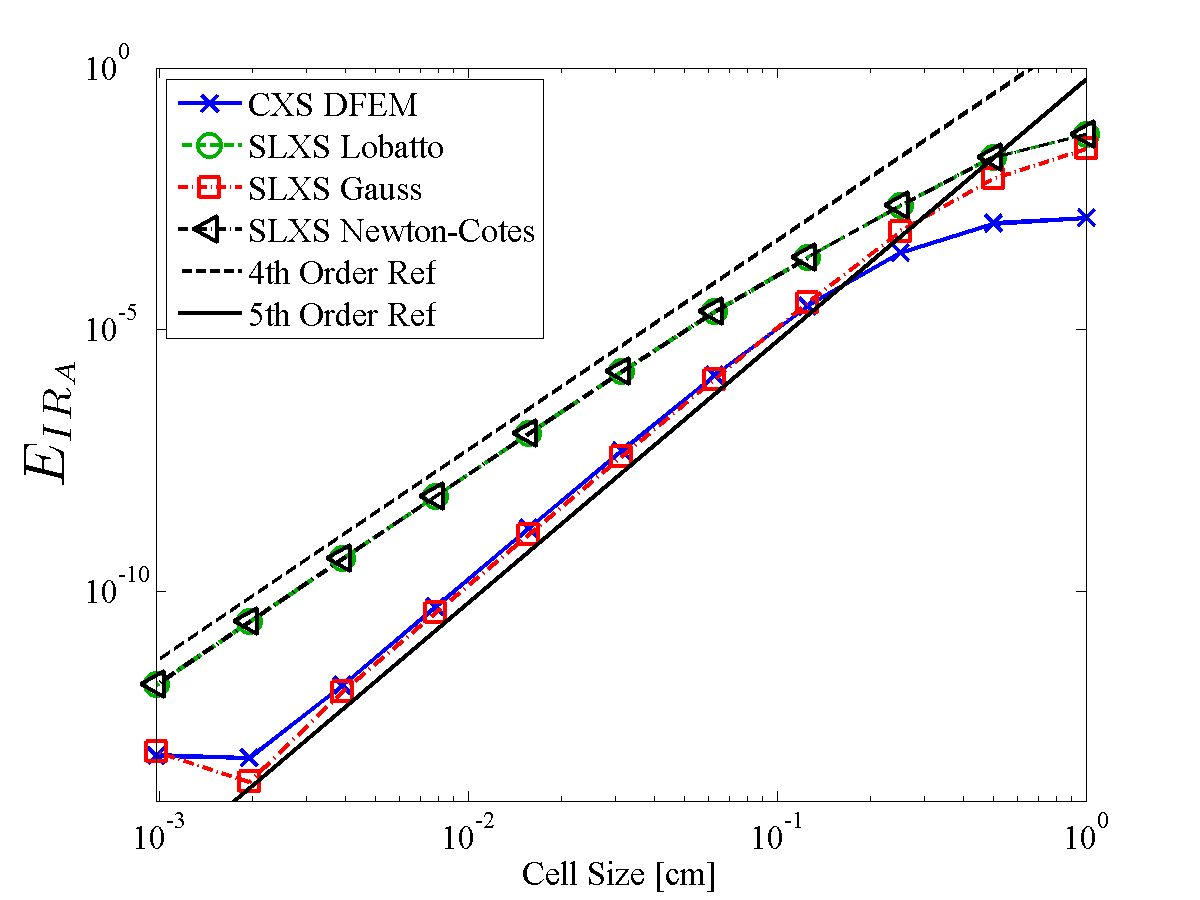
\includegraphics[width=11cm]{chapter3_variable_xs/P2_VarXS_E_I_A.png}
}
\subfigure[Cubic]{
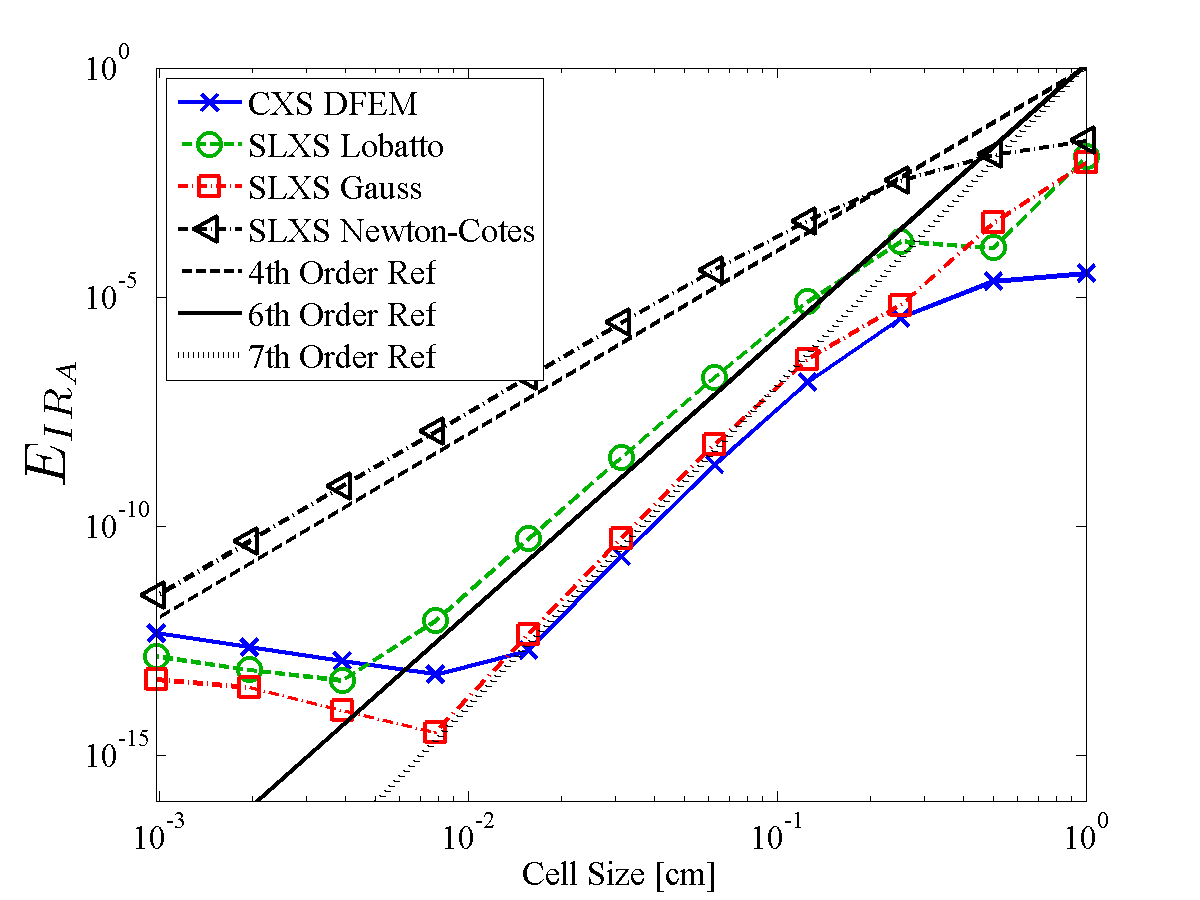
\includegraphics[width=11cm]{chapter3_variable_xs/P3_VarXS_E_I_A.png}
}
\subfigure[4-th Order]{
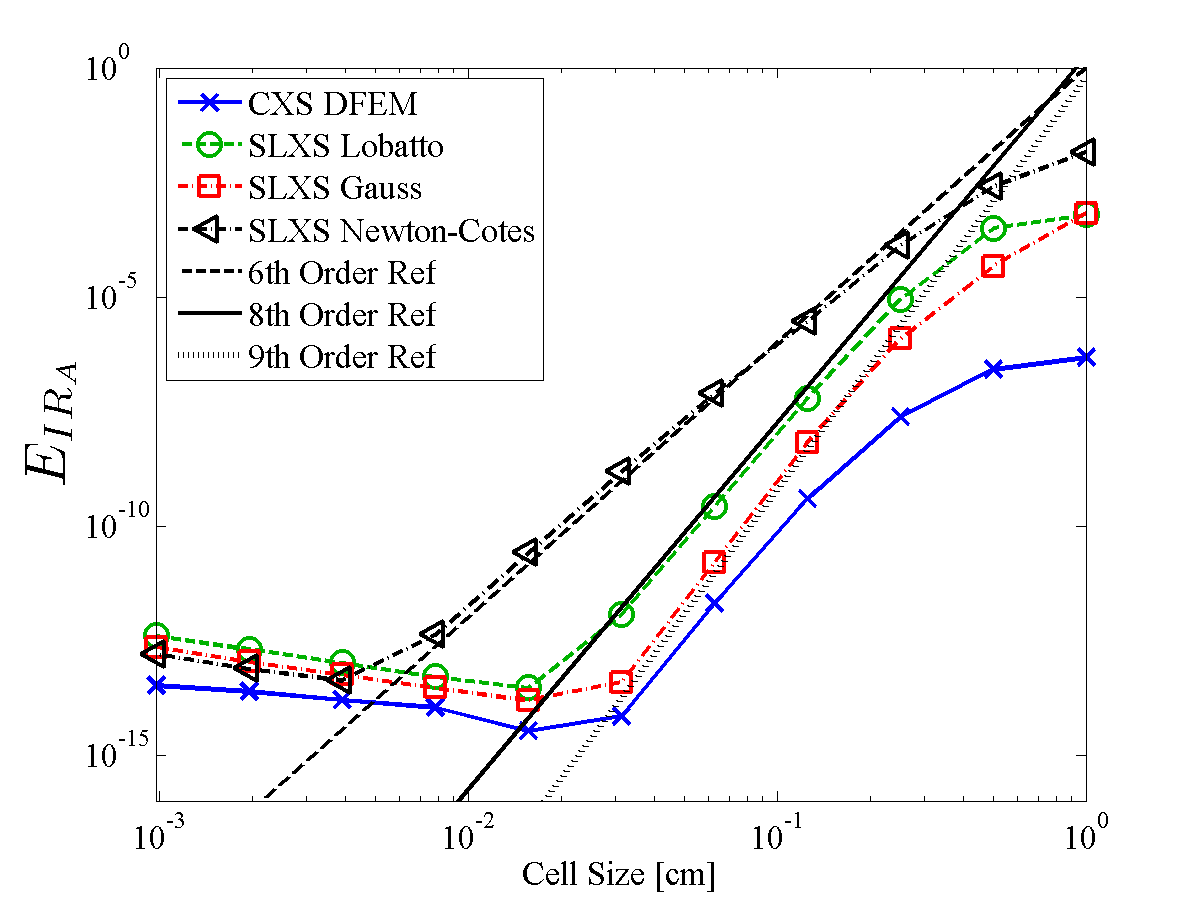
\includegraphics[width=11cm]{chapter3_variable_xs/P4_VarXS_E_I_A.png}
}
\end{center}
\caption{Convergence of $E_{IR_A}$ for a multiple cell problem as a function of cell size for a pure absorber with exponentially varying cross section, $c_1 = 0.1~[cm^{-1}]$, $c_2 = 2\ln(10)~[cm^{-1}]$, and $x\in \left[0,1~[cm] \right]$.}
\label{fig:varxs_I_A}
\end{figure}
The plateauing of numerical errors for various high-order methods using very small cell sizes in Figs. \ref{fig:varxs_psi_L2}-\ref{fig:varxs_I_A} is a consequence of having  reached machine precision.
The lines in Figs. \ref{fig:varxs_psi_L2}-\ref{fig:varxs_I_A} that extend to values smaller than machine precision are reference lines.

Figures \ref{fig:varxs_psi_L2}-\ref{fig:varxs_psi_out} show that, for a linear angular flux trial space, CXS DFEM achieves the same orders of spatial convergence as observed with Exact DFEM in \cite{part_1_paper}.
However, as the degree of the DFEM trial space is increased, the CXS DFEM scheme does not show an increase in the order of the spatial convergence rate of  $E_{\psi}$ and $E_{\psi_A}$; the convergence rate of CXS DFEM is limited to at most second order for both $E_{\psi}$ and $E_{\psi_A}$, regardless of the trial space polynomial degree.  
The increase in order of convergence of CXS DFEM for $E_{\psi_{out}}$ as trial space is increased is a result of angular flux outflow in the
CXS DFEM discretization being only a function of the cell optical thickness, which is preserved exactly by our definition of $\hat{\Sigma}_t$; see \eqt{eq:chap3_cxs_sigma}.

Of the self-lumping schemes, SLXS Newton-Cotes is the least accurate.  SLXS Newton-Cotes convergence of $E_{\psi}$ is limited to at most second order for odd degree polynomial trial spaces and third order for even degree trial spaces.  
Convergence of $E_{\psi_A}$ and $E_{\psi_{out}}$ for the SLXS Newton-Cotes scheme generally increases with an increase in the DFEM polynomial trial space degree, but is only proportional to $P$.

Both SLXS Lobatto and SLXS Gauss converge $E_{\psi}$, $E_{\psi_A}$, and $E_{\psi_{out}}$ similarly to the study carried out in \cite{part_1_paper} with a spatially constant cross section.
The spatial convergence of $E_{\psi}$ for SLXS Lobatto and SLXS Gauss is order $P+1$.
Though SLXS Lobatto and SLXS Gauss converge with the same order of spatial convergence for $E_{\psi}$, SLXS Gauss is more accurate than SLXS Lobatto by a constant.  
SLXS Gauss converges $E_{\psi_A}$ and $E_{\psi_{out}}$ $\propto 2P+1$, whereas SLXS Lobatto converges both $\propto 2P$.
SLXS Gauss and SLXS Lobatto converge angular flux error quantities for the case of a spatially varying cross section with the same rates of convergence as their constant cross-section analogs did in \cite{part_1_paper}.
This suggests that exactly integrating the interaction term in the DFEM moment equations is not essential for developing arbitrarily high-order accuracy DFEM schemes for radiation transport.

We observe the detrimental effect of approximating a spatially varying cross section with a constant in each spatial cell when we examine the $L_2$ convergence results for the interaction rate, $E_{IR}$, for the CXS DFEM scheme.
Regardless of angular flux trial space polynomial degree, CXS DFEM converges $E_{IR}$ to only first order in space.
However, the self-lumping schemes exhibit the same trends in converging $E_{IR}$ (in the $L^2$-norm sense) as exhibited in converging $E_{\psi}$:
\begin{itemize}
\item SLXS Lobatto and SLXS Gauss converge $E_{IR}$ with order $P+1$,
\item SLXS Gauss is more accurate than SLXS Lobatto by a constant, and
\item SLXS Newton-Cotes converges $E_{IR}$ second order in space for odd degree trial spaces and third order in space for even degree trial spaces.
\end{itemize}  

The convergence results of the cell average interaction rate, $E_{IR_A}$, shown in \fig{fig:varxs_I_A}, do not behave as intuitively.  Given the poor performance of CXS DFEM in converging $E_{IR}$, one would expect that CXS DFEM would converge $E_{IR_A}$ poorly as well.  
However, this is not the case and CXS DFEM converges $E_{IR_A}$ with the same order of convergence as the best performing self-lumping scheme considered.
CXS DFEM converges $E_{IR_A}$ with a high-order of accuracy because of the locally conservative properties of DFEM approximations, that is:
\benum
\text{Particles Into Cell} - \text{Particles Out of Cell} =  \text{Total Interactions in Cell} \pep
\label{eq:chap3_balance}
\eenum
As shown in \fig{fig:varxs_psi_out}, CXS DFEM converges the quantities on the left hand side of \eqt{eq:chap3_balance} with the same order of accuracy as any self-lumping scheme considered; CXS DFEM is at least as accurate in calculating the particles into a cell (outflow from the previous cell) and out of the cell (outflow from the current cell) as any other scheme considered.
Since \eqt{eq:chap3_balance} holds regardless of the numerical scheme considered, it follows that CXS DFEM converges $E_{IR_A}$, the term in the right hand side of \eqt{eq:chap3_balance} summed over all cells, with the maximum order of convergence displayed by any of the DFEM schemes we consider here.
\fig{fig:varxs_I_A} validates this conclusion.
CXS DFEM and SLXS Gauss exhibit the highest order of spatial convergence, converging $E_{IR_A}$ with order $\propto 2P + 1$.  
SLXS Newton-Cotes and SLXS Lobatto converge $E_{IR_A}$ with the same orders of convergence each method exhibits in converging $E_{\psi_A}$ for this problem with SLXS Lobatto converging $\propto 2P$ and SLXS Newton-Cotes $\propto P$.

%%%%%%%%%%%%%%%%%%%%%%%%%%%%%%%%%%%%%%%%%%%%%%%%%%%%%%%%%%%%%%%%%%%%%
\subsection{Consequences of Assuming a Cell-Wise Constant Cross Section}
%%%%%%%%%%%%%%%%%%%%%%%%%%%%%%%%%%%%%%%%%%%%%%%%%%%%%%%%%%%%%%%%%%%%%

To understand the poor convergence of point-wise error in angular flux and interaction rate, $E_{\psi}$ and $E_{IR}$, associated with CXS DFEM  we now examine more closely the CXS DFEM spatial approximations to $\psi(x,\mu_d)$ and $IR(x)$. 
We again consider a pure absorber with total absorption cross section that varies exponentially in space with $c_1 = 0.1$, and $c_2 = 2\ln(10)$.  
A beam of radiation is incident on the left face in the direction of $\mu_d=1$, vacuum boundary conditions are applied on the right face of the slab, and $x\in[0, 1]$.    

In \fig{fig:cxs_blades}, we plot the exact $\psi(x)$ and $IR(x)$, as well as their CXS DFEM numerical approximations, $\widetilde{\psi}(x)$ and $\widetilde{IR}(x)$, using $N_{cells}=5$, and $\hat{\Sigma}_{t,i}$ as defined in \eqt{eq:chap3_cxs_sigma}. 
Additionally, we plot the analytic angular flux and reaction rate one would obtain if the cell average cross section, $\hat{\Sigma}_{t,i}$, had been used instead of the true $\Sigma_t(x)$.
We refer to these analytic solutions as $\psi_C(x)$ and $IR_C(x)$.
\begin{figure}[!htp]
\begin{center}
\subfigure[Angular Flux]{
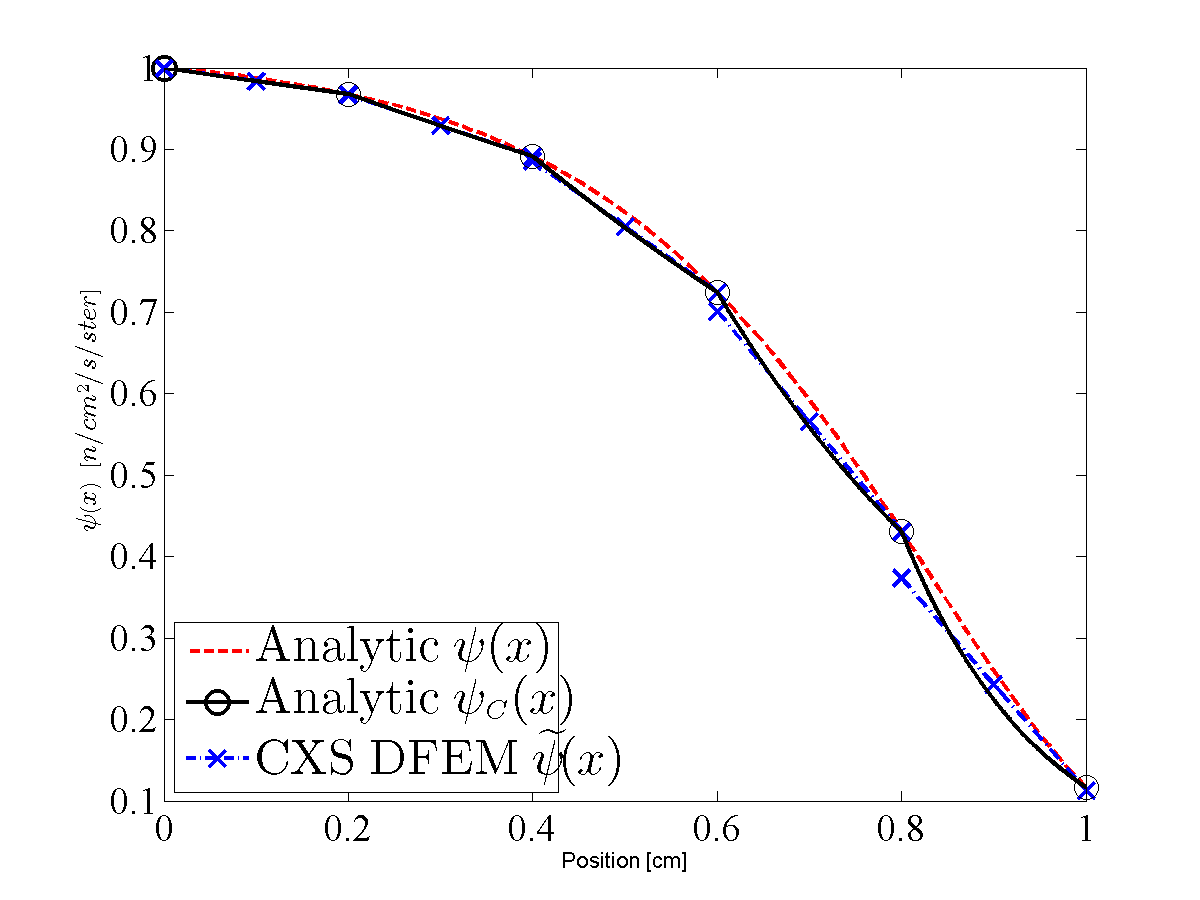
\includegraphics[width=11cm]{chapter3_variable_xs/Psi_Blades.png}
\label{fig:cxs_blades_a}
}
\subfigure[Reaction Rate]{
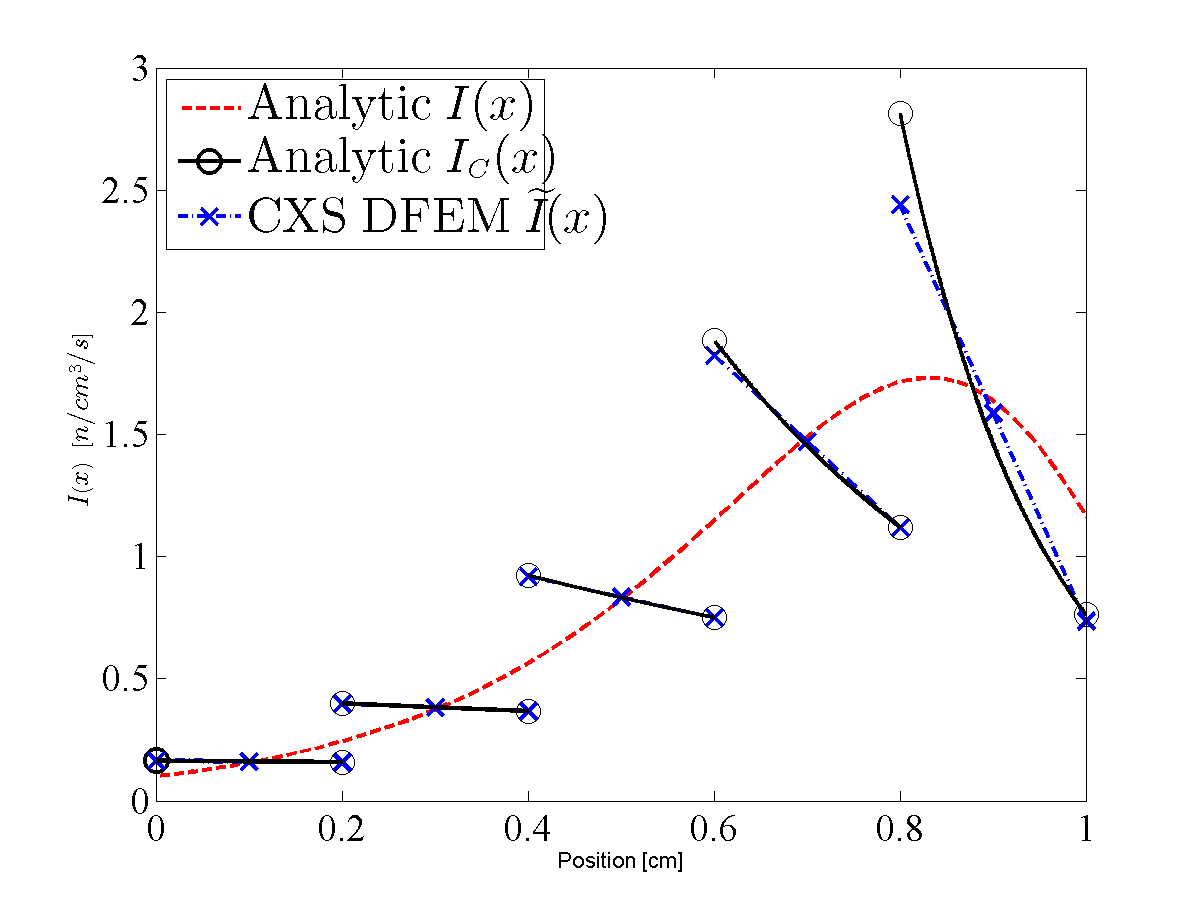
\includegraphics[width=11cm]{chapter3_variable_xs/I_Blades.png}
}
\end{center}
\caption{Plots of the analytic $\psi(x)$ and $IR(x)$ and the CXS DFEM $\widetilde{\psi}(x)$ and $\widetilde{IR}(x)$ for the pure absorber with exponential cross section.  Also shown are the analytic $\psi_C(x)$ and $IR_C(x)$ solutions.}
\label{fig:cxs_blades}
\end{figure}
%%
%%if instead of being the exponentially varying $\Sigma_t(x)$, total macroscopic cross section, was a piecewise constant function, $\Sigma_{t,C}(x)$, equal to $\hat{\Sigma}_{t,i}$, such that:
%%\benum
%%\Sigma_{t,C}(x) = \frac{1}{\Delta x_i}\int_{x_{i-1/2}}^{x_{i+1/2}}{\Sigma_1 A^{\Sigma_2 x}~dx},~~x\in[x_{i-1/2},x_{i+1/2}] \pec
%%\eenum
%%where $x_{i\pm1/2}$ are the boundaries of cell $i$ used in by the CXS DFEM scheme.
%%We refer to the analytic angular flux and interaction rate solutions of the problem where total macroscopic cross section is $\Sigma_{t,C}(x)$ as $\psi_C(x)$ and $I_C(x)$, respectively.

Since CXS DFEM is a discontinuous scheme, some discontinuity is expected in the plots of $\widetilde{\psi}$ and $\widetilde{IR}$ in \fig{fig:cxs_blades}. 
However, the discontinuities present in $\widetilde{IR}(x)$ of \fig{fig:cxs_blades} are highly disconcerting.
The analytic $IR(x)$ is smooth and does not vary rapidly within individual mesh cells, yet there are significant, non-monotonic discontinuities in the CXS DFEM interaction rate solution to the pure absorber problem with exponentially varying cross section.
The noticeably poor behavior of $\widetilde{IR}(x)$ in \fig{fig:cxs_blades} is inherent to the assumption of a cell-wise constant cross section.
%The inherent error of approximating a continuously varying cross section with cell-wise constants 
This is clearly visible in \fig{fig:cxs_blades} when $\psi(x)$ and $IR(x)$, calculated assuming a spatially varying cross section, are compared to the analytic solutions assuming a cell average cross section, $\psi_C(x)$ and $IR_C(x)$. 
%The only difference between these two sets of results is the approximation of $\Sigma_t(x) \approx \hat{\Sigma}_{t,i}$.
Figure \ref{fig:cxs_blades} does not suggest that linear DFEM is unsuitable for use in problems with spatially varying cross sections. 
Rather, comparing the CXS DFEM $\widetilde{\psi}(x)$ and $\widetilde{IR}(x)$ to $\psi_C(x)$ and $IR_C(x)$ in \fig{fig:cxs_blades_a}, we see that CXS DFEM  is very accurate when the problem is assumed to have piece-wise constant, cell averaged cross sections.

Given the poor accuracy of CXS DFEM in approximating the true $\psi(x)$ and $IR(x)$, consider $\widetilde{\psi}(x)$ and $\widetilde{IR}(x)$ obtained with SLXS Lobatto using a linear DFEM trial space and five spatial cells, shown in \fig{fig:lobatto_blades}, for the same problem.  
In \fig{fig:lobatto_blades}(a), the differences between the angular flux solutions obtained using (1) a cell-wise constant cross section (CXS DFEM) and (2) evaluating cross section values at quadrature points (SLXS Lobatto) are small.
\begin{figure}[!htp]
\begin{center}
\subfigure[Angular Flux]{
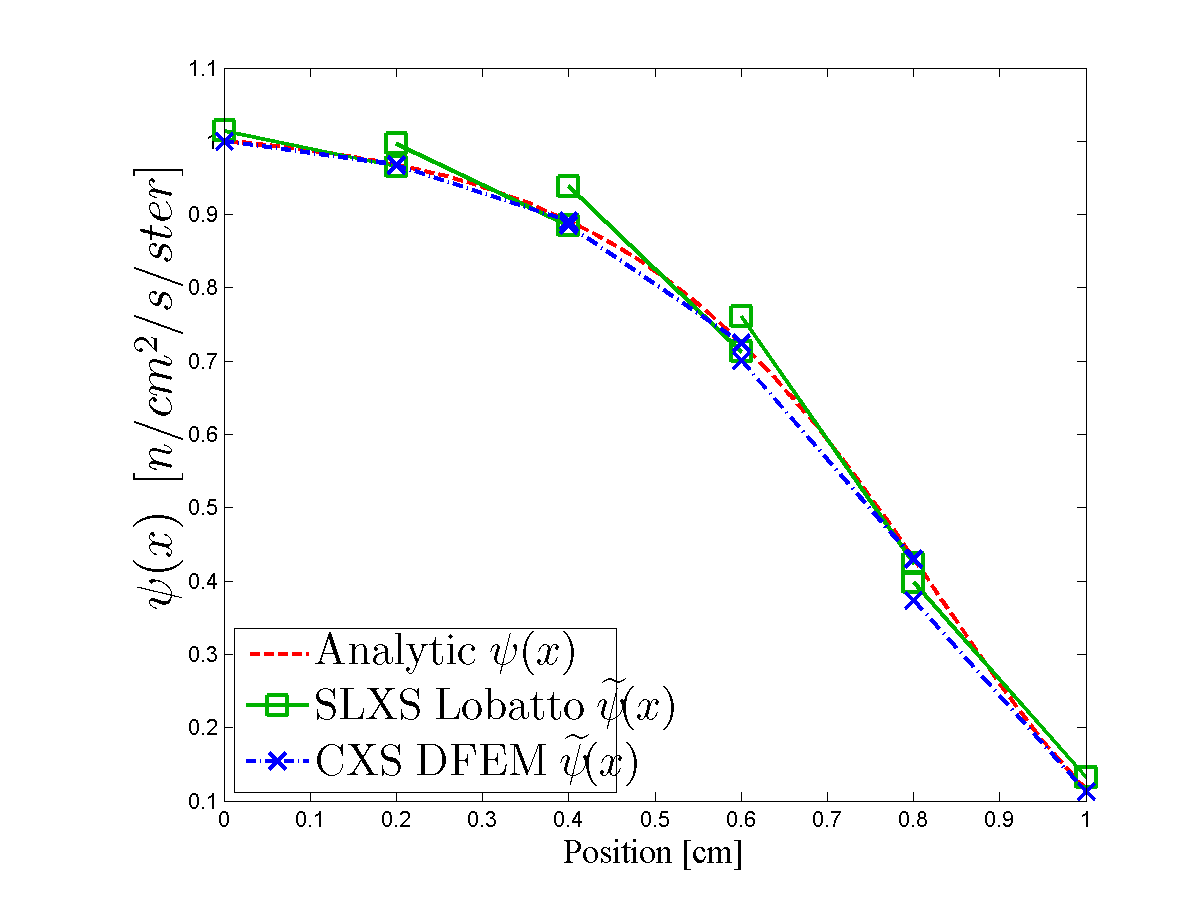
\includegraphics[width=11cm]{chapter3_variable_xs/SLXS_Psi_Profile.png}
}
\subfigure[Reaction Rate]{
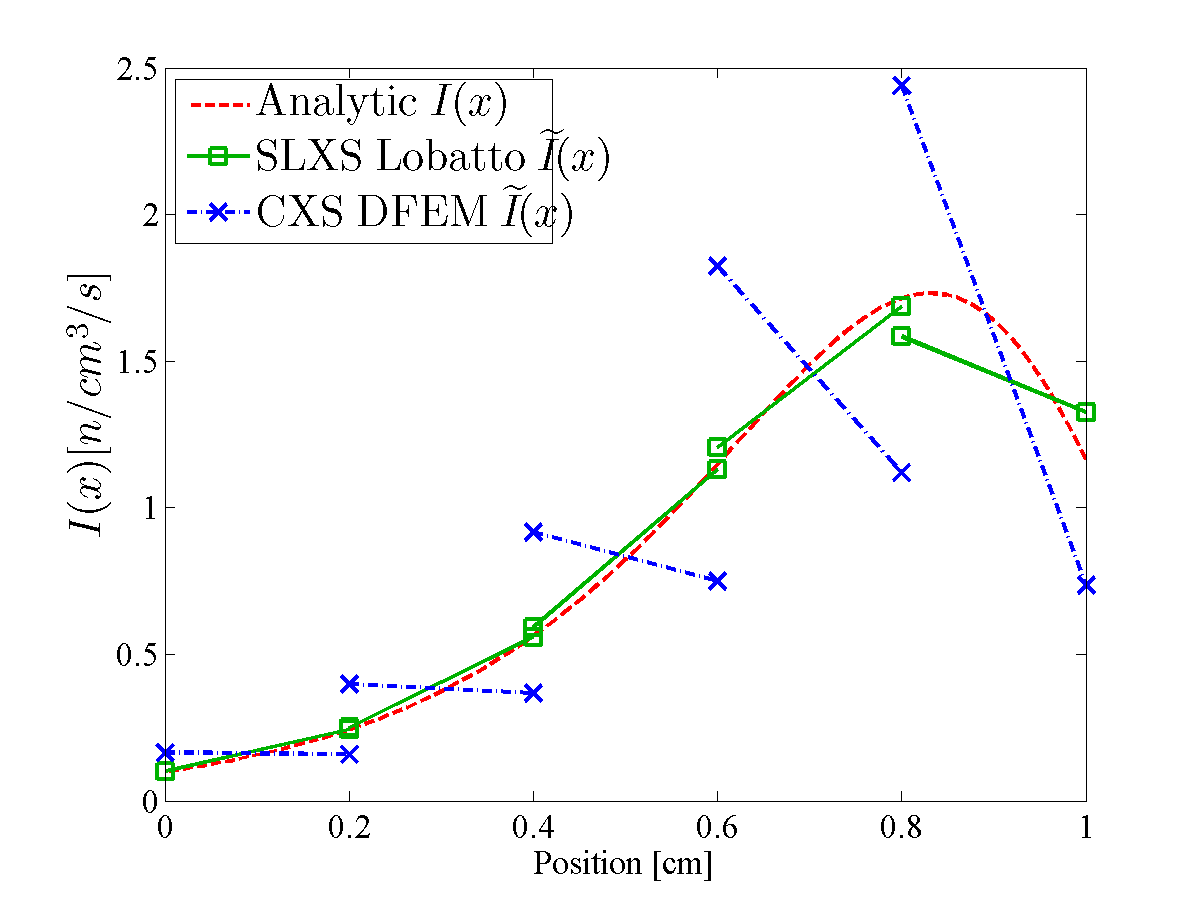
\includegraphics[width=11cm]{chapter3_variable_xs/SLXS_I_Profile.png}
}
\end{center}
\caption{Plot of the linear trial space SLXS Lobatto and CXS DFEM approximations $\widetilde{\psi}(x)$ and $\widetilde{IR}(x)$ for the pure absorber problem with exponentially varying cross section.}
\label{fig:lobatto_blades}
\end{figure}
This is not the case when comparing the different approximations to the interaction rate, $\widetilde{IR}(x)$, in \fig{fig:lobatto_blades}(b).  
Though there are discontinuities in the SLXS Lobatto $\widetilde{IR}(x)$, the discontinuities are smaller and the SLXS Lobatto $\widetilde{IR}(x)$ is monotonic unlike the CXS DFEM $\widetilde{IR}(x)$.   
The SLXS Lobatto $\widetilde{IR}(x)$ is clearly more accurate than the CXS DFEM $\widetilde{IR}(x)$.
%
%
In this problem, there are two possible sources of error that could cause a DFEM to be inaccurate: inexact matrix evaluation and not incorporating cross-section spatial variation into the scheme.
By definition, CXS DFEM exactly integrates the mass matrix, and we showed in \cite{part_1_paper} that schemes which exactly integrate the mass matrix are more accurate than schemes that only approximately integrate the mass matrix, like SLXS Lobatto.
Thus, the poor accuracy of CXS DFEM relative to SLXS Lobatto is entirely caused by the approximation of a spatially varying cross section with a cell-wise constant value.

The ``blading'' in $\widetilde{IR}(x)$ has not previously been reported in the radiation transport literature.
We are likely not the first to have generated these large, non-monotonic discontinuities. 
In fact, we believe that blading has frequently been present in DFEM radiation transport simulations and literature, but has likely gone unnoticed due to the prevalence of linear DFEM and simplified data visualization using cell midpoint values.
Consider \fig{fig:cxs_avg}(a) and \fig{fig:cxs_avg}(b) that linearly interpolate between $\widetilde{\psi}_{A,i}$ and  $\widetilde{IR}_{A,i}$ plotted at cell centers.
\begin{figure}[!htp]
\begin{center}
\subfigure[Angular Flux]{
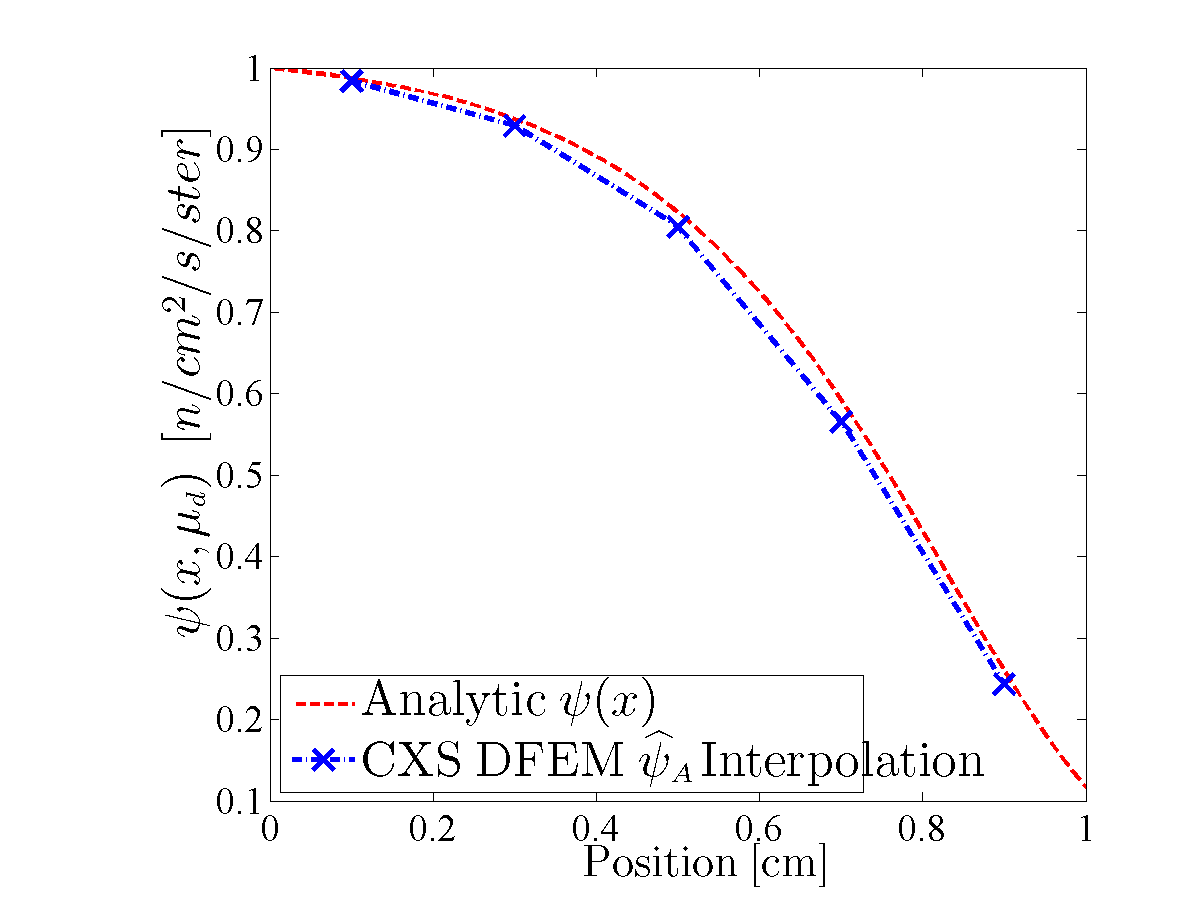
\includegraphics[width=11cm]{chapter3_variable_xs/CXS_Psi_A_Profile.png}
}
\subfigure[Reaction Rate]{
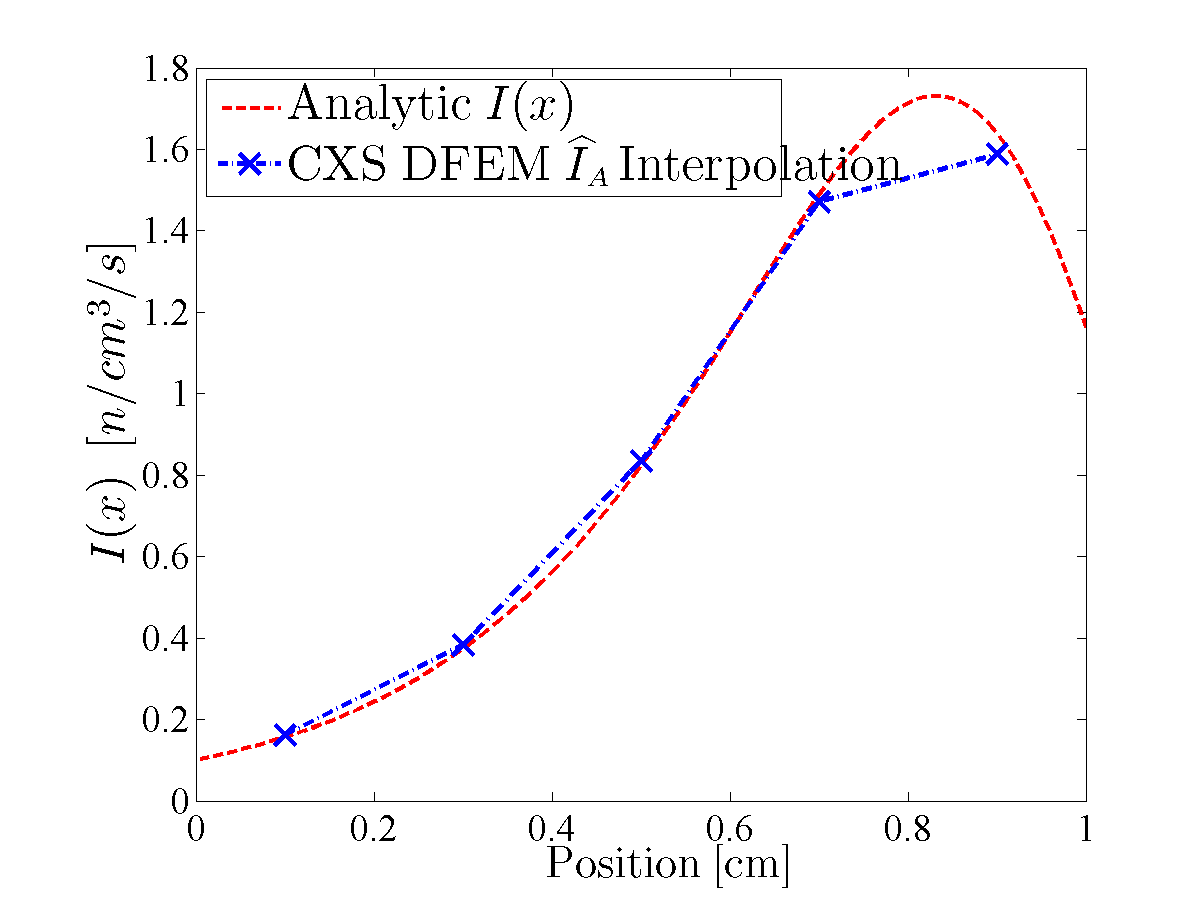
\includegraphics[width=11cm]{chapter3_variable_xs/CXS_I_A_Profile.png}
}
\end{center}
\caption{Plot of the CXS DFEM cell average angular fluxes and interaction rates at cell centers with linear interpolation for a pure absorber with a spatially varying cross section.}
\label{fig:cxs_avg}
\end{figure}
While \fig{fig:cxs_avg}(a) is visually indistinguishable from \fig{fig:cxs_blades}(a), the blading of $\widetilde{IR}(x)$ present in \fig{fig:cxs_blades}(b) is not at all visually present in \fig{fig:cxs_avg}(b).
%
%Note that for linear DFEM and cell-wise constant cross sections, $\widetilde{\psi}_{A,i}$ and $\widetilde{IR}_{A,i}$ are equivalent to $\widetilde{\psi}(s)$ and $\widetilde{IR}(s)$ evaluated at $s=0$.  
%It is therefore reasonable to approximately plot $\widetilde{\psi}(s)$ and $\widetilde{IR}(s)$ by plotting $\widetilde{\psi}_{A,i}$ and $\widetilde{IR}_{A,i}$ at $x_i$ and linearly interpolating.
%Figure \ref{fig:cxs_avg}, plots the same data used to generate \fig{fig:cxs_blades}, but uses only cell average quantities plotted at cell centers.
%Because the differences between CXS DFEM $\widetilde{\psi}$ and $\psi(x)$ are relatively small the approximate plot of the CXS DFEM $\widetilde{\psi}(x)$ in \fig{fig:cxs_avg}(a) is essentially visually identical to the plot of $\widetilde{\psi}(x)$ in \fig{fig:cxs_blades}(a).  
%This similarity increases as finer mesh results plotted in the same manner are compared.
%But by changing the $\widetilde{IR}(x)$ plotting method, one's opinion of the quality of the CXS DFEM interaction rate approximation, $\widetilde{IR}(x)$, changes greatly.
%The modified plotting technique in \fig{fig:cxs_avg}(b) shows a scheme that appears to be accurate and well behaved, whereas the same numerical data presented as the true CXS DFEM $\widetilde{IR}(x)$, in \fig{fig:cxs_blades}(b), shows a scheme that is both inaccurate and poorly behaved.

Interaction rate terms are present in other radiation transport physics.
In particular, we think of the radiative transfer analog to the neutronics interaction rate, absorption rate density.
 %term in the radiative transfer material energy equation.
%The constant cross section approximation for a neutronics problem with spatially varying cross section resulted in interaction rate profile blading; 
%We hypothesize that assuming cell-wise constants opacities for problems with spatially/temperature dependent opacities could introduce blading in radiative transfer temperature solutions, via the material energy equation's absorption rate density term.
%%, with , degrading overall solution accuracy.
%%In preliminary radiative transfer studies of Marshak wave type problems like those in \cite{ober_shadid}, we have observed that by using a lumped linear discontinuous finite element spatial discretization of both the temperature and intensity and assuming a constant opacity within each cell as proposed by Morel, et. al. in \cite{morel_radtran}, leads to a temperature profile that exhibits blading, not only at the wave front, but after the wave front has passed and the material has been heated by the incident radiation.
%However, like the interaction rate profile in neutronics, linearly interpolating cell average temperatures (plotted at cell centers) has prevented temperature solution blading from being observed.
%%
%%It is our belief that we are not the first to encounter the blading phenomena in our radiative transfer calculations.  
%%Rather, we believe that radiative transfer results from schemes similar to \cite{morel_radtran} which have assumed cell-wise constant opacities, have plotted cell average temperatures
%%at cell centers and linearly interpolated, instead of plotting the true $\widetilde{T}(x)$, causing none of the discontinuities to be observed.

%%%%%%%%%%%%%%%%%%%%%%%%%%%%%%%%

\subsection{Flux-Weighting versus Volume-Averaged Cross Sections}

In our results thus far, we have only considered volume-averaged cell-wise cross sections(the CXS DFEM scheme).
However, in reactor physics problems, a flux-weighted cross section is often used to generate spatially averaged cross sections \cite{bell_glasstone}.
We now introduce the flux-weighted cell-wise constant cross section scheme (FW CXS), which differs from the CXS DFEM scheme only by how $\hat{\Sigma}$ is defined in each cell: 
\benum
\hat{\Sigma}_i = \frac{\int_{x_{i-1/2}}^{x_{i+1/2}}{ \Sigma(x) \psi(x,\mu_d)~dx}}{\int_{x_{i-1/2}}^{x_{i+1/2}}{ \psi(x,\mu_d)~dx}} \pep
\label{eq:chap3_fw_cxs}
\eenum
In practice, flux-weighting is often done using the scalar flux in order not to have angle-dependent total cross section.  However for the beam problem considered here, $\psi(x,\mu_d)$ is proportional to the scalar flux.

We first compare the accuracy of FW CXS versus  volume-averaged CXS DFEM for a cubic DFEM trial space, as shown in \fig{fig:fw_accuracy}.  
%In \fig{fig:fw_accuracy}, we omit a plot of $E_{\psi_{out}}$ as we have already demonstrated that the accuracy of any method in calculating $E_{\psi_{out}}$ determines the method's accuracy in calculating $E_{IR_A}$.  
%That is, if $E_{IR_A}$ converges at a given rate, $E_{\psi_{out}}$ converges at the same rate.  

Figure \ref{fig:fw_accuracy} shows that FW CXS scheme is more accurate than CXS DFEM when comparing $E_{\psi}$, $E_{\psi_A}$ and, at low resolutions, for $E_{IR}$.
However, though designed to preserve cell average interaction rates, FW CXS scheme is not only less accurate than  CXS DFEM in calculating cell average interaction rates, it converges at most second order in space, whereas a volume-averaged cross section converges $\propto 2P+1$ for the pure absorber problem.
\begin{figure}[!htp]
\begin{center}
\subfigure[$E_{\psi}$]{
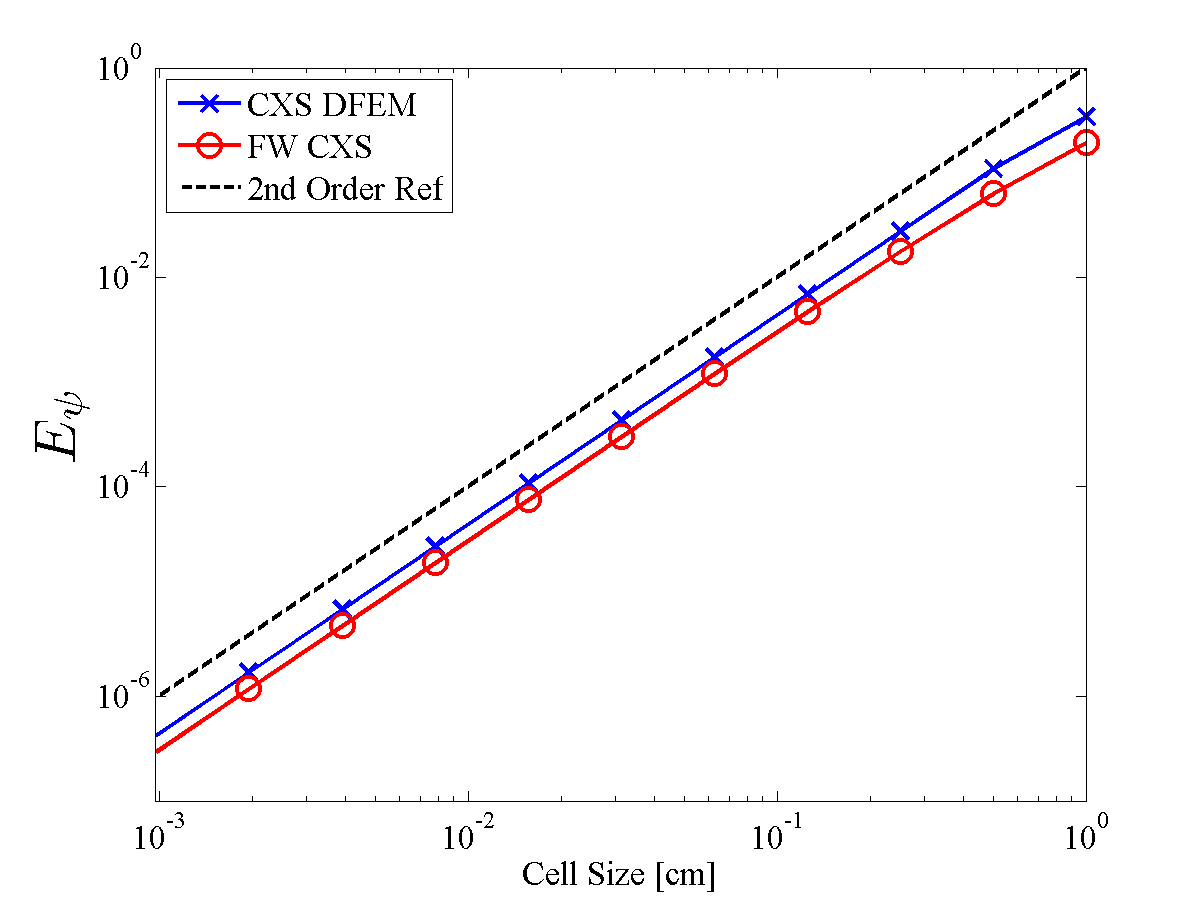
\includegraphics[width=11cm]{chapter3_variable_xs/FW_XS_P3_VarXS_E_psi_L2.png}
}
\subfigure[$E_{\psi_A}$]{
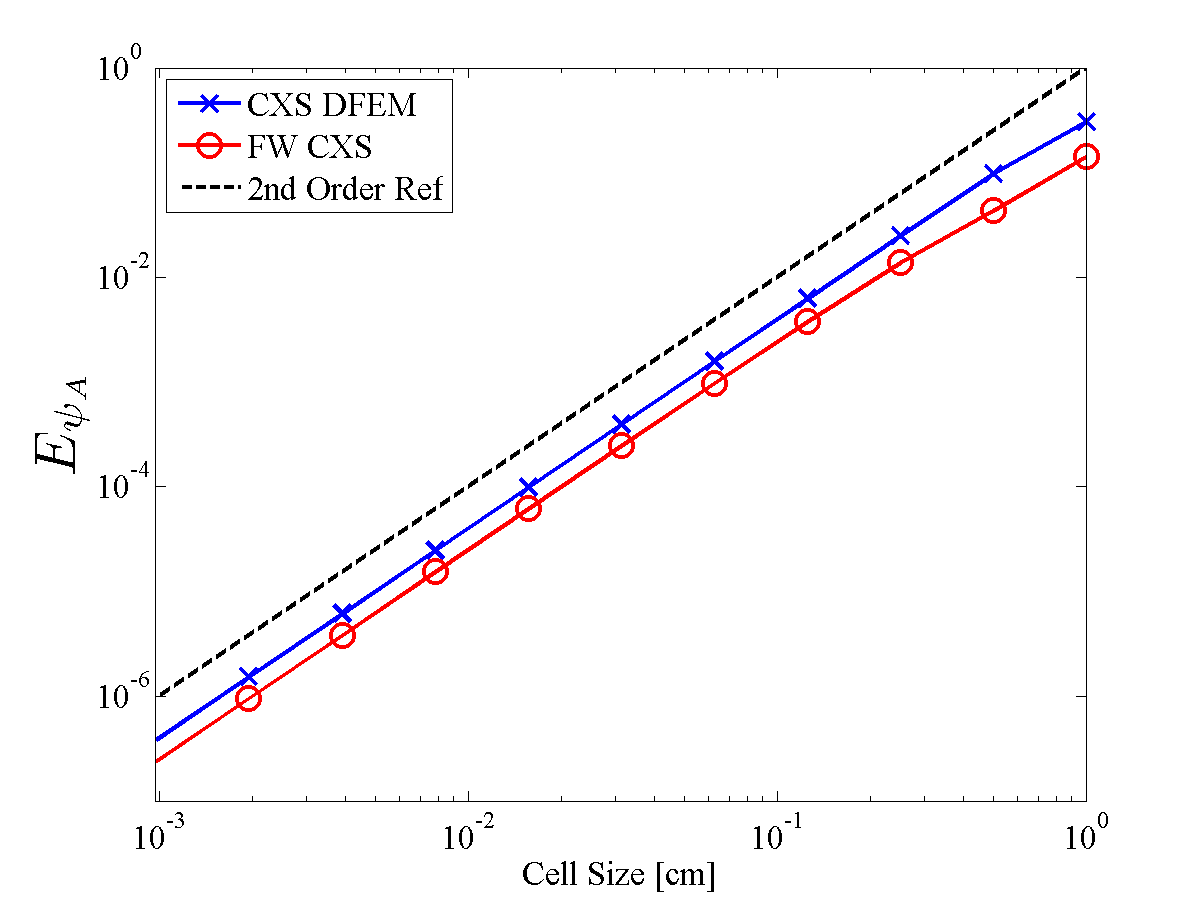
\includegraphics[width=11cm]{chapter3_variable_xs/FW_XS_P3_VarXS_E_psi_A.png}
}
\subfigure[$E_{IR}$]{
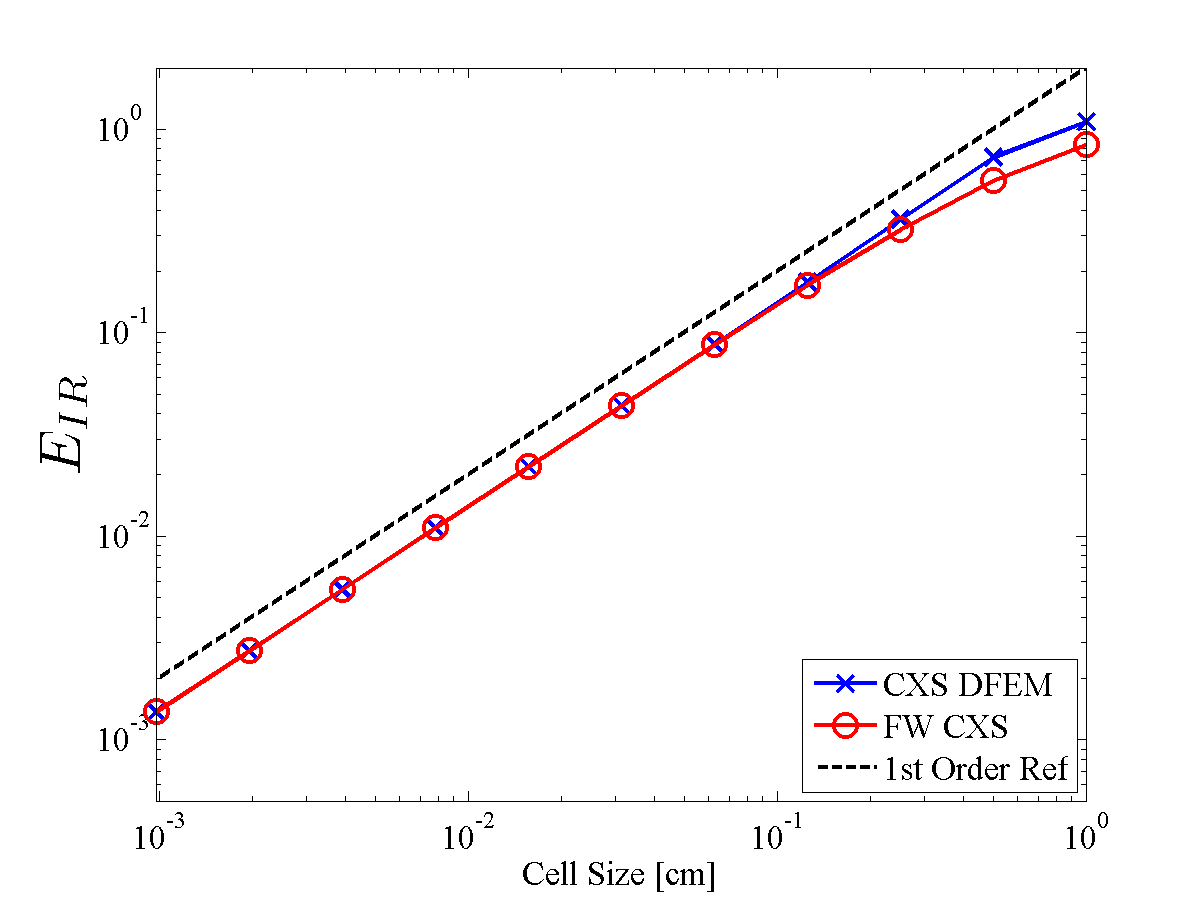
\includegraphics[width=11cm]{chapter3_variable_xs/FW_XS_P3_VarXS_E_I_L2.png}
}
\subfigure[$E_{IR_A}$]{
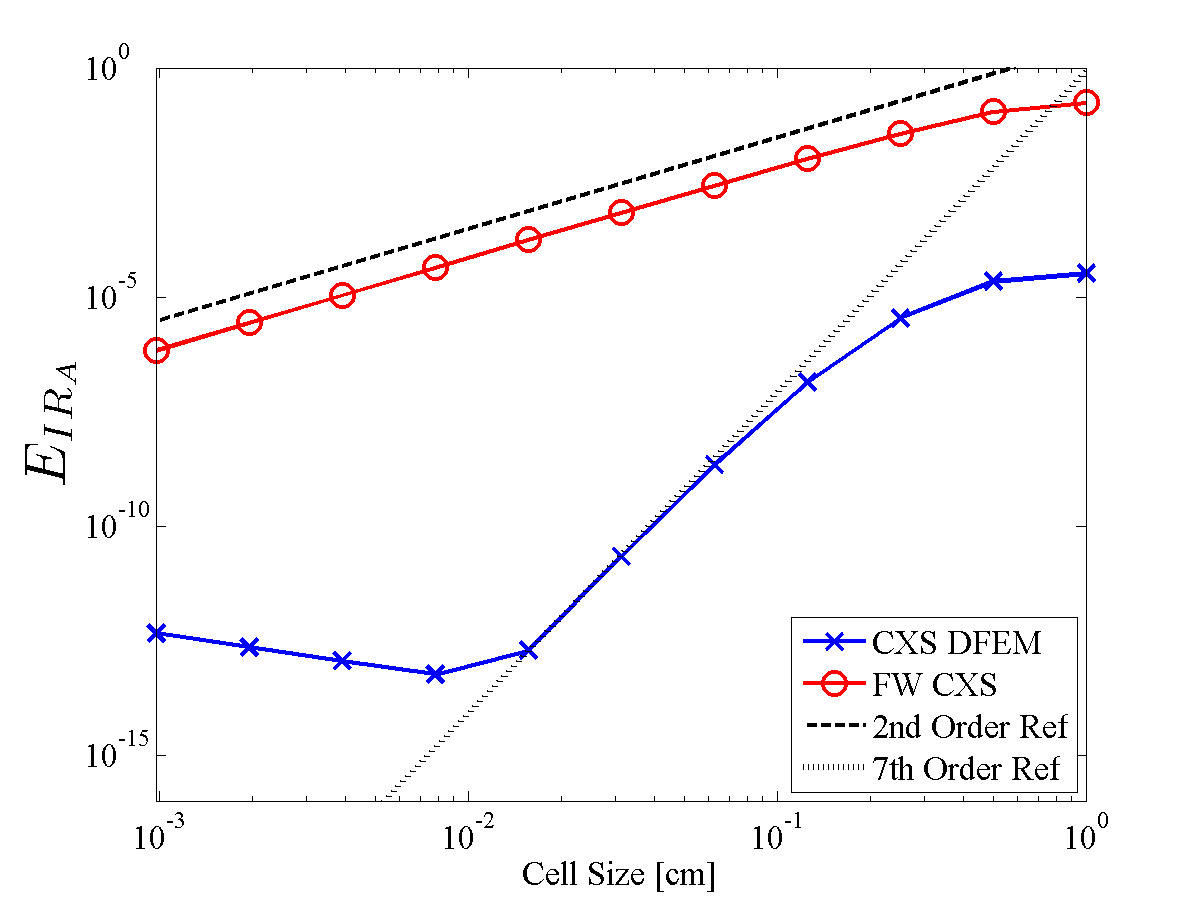
\includegraphics[width=11cm]{chapter3_variable_xs/FW_XS_P3_VarXS_E_I_A.png}
}
\end{center}
\caption{Accuracy comparison of flux weighted constant cross section scheme (FW CXS) to volume averaged cross section  scheme (CXS DFEM) with a cubic angular flux trial space.}
\label{fig:fw_accuracy}
\end{figure}
Finally, we consider the $\widetilde{\psi}_d(x)$ and $\widetilde{IR}(x)$ solution representations of the FW CXS scheme.  
In \fig{fig:fw_blading} it is clear that while the FW CXS and CXS DFEM schemes calculate slightly different solution representations, the FW CXS scheme  exhibits the same interaction rate blading phenomena as the CXS DFEM scheme, reiterating that blading is a result of approximating a spatially varying cross section with as a cell-wise constant.
The choice of cell-wise cross section does not eliminate blading.
\begin{figure}[!htp]
\begin{center}
\subfigure[Angular Flux]{
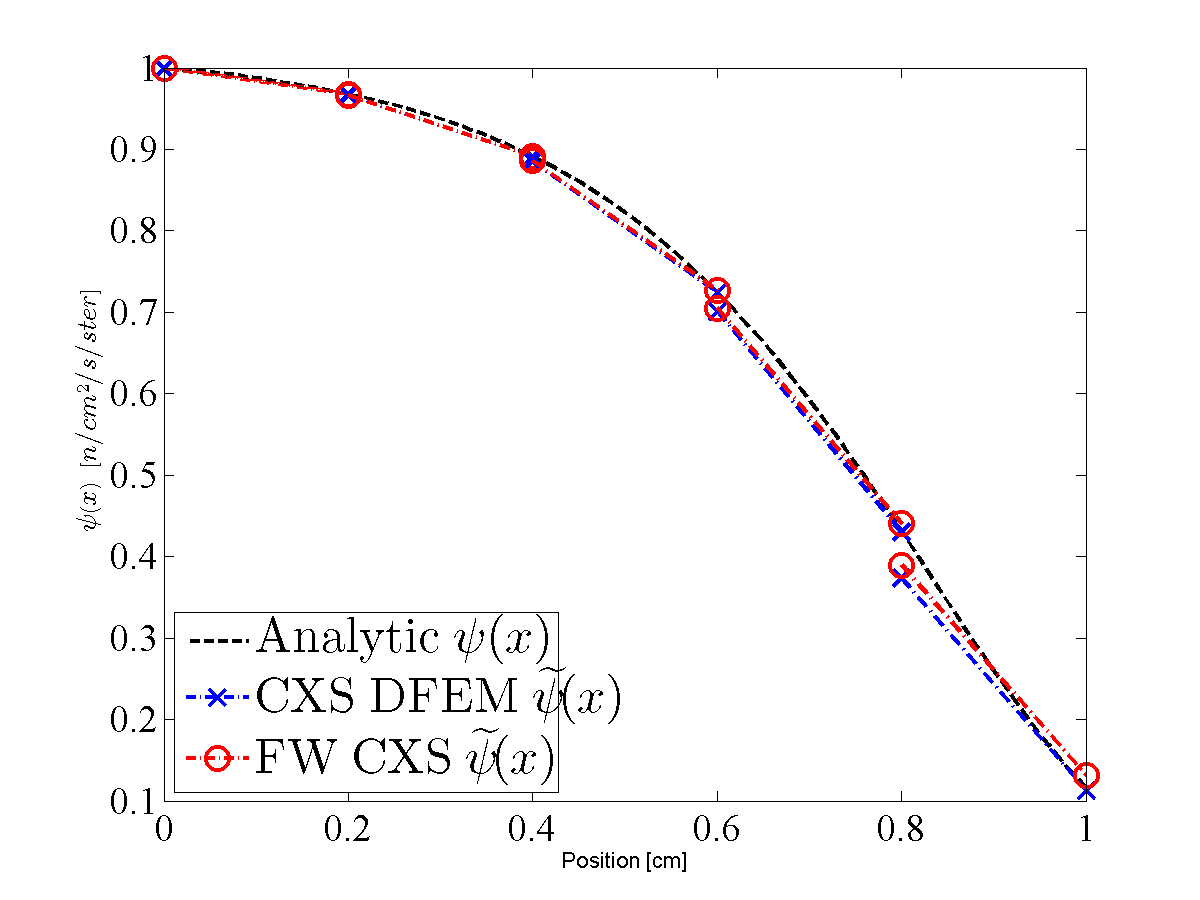
\includegraphics[width=11cm]{chapter3_variable_xs/FW_Psi_Blades.png}
}
\subfigure[Reaction Rate]{
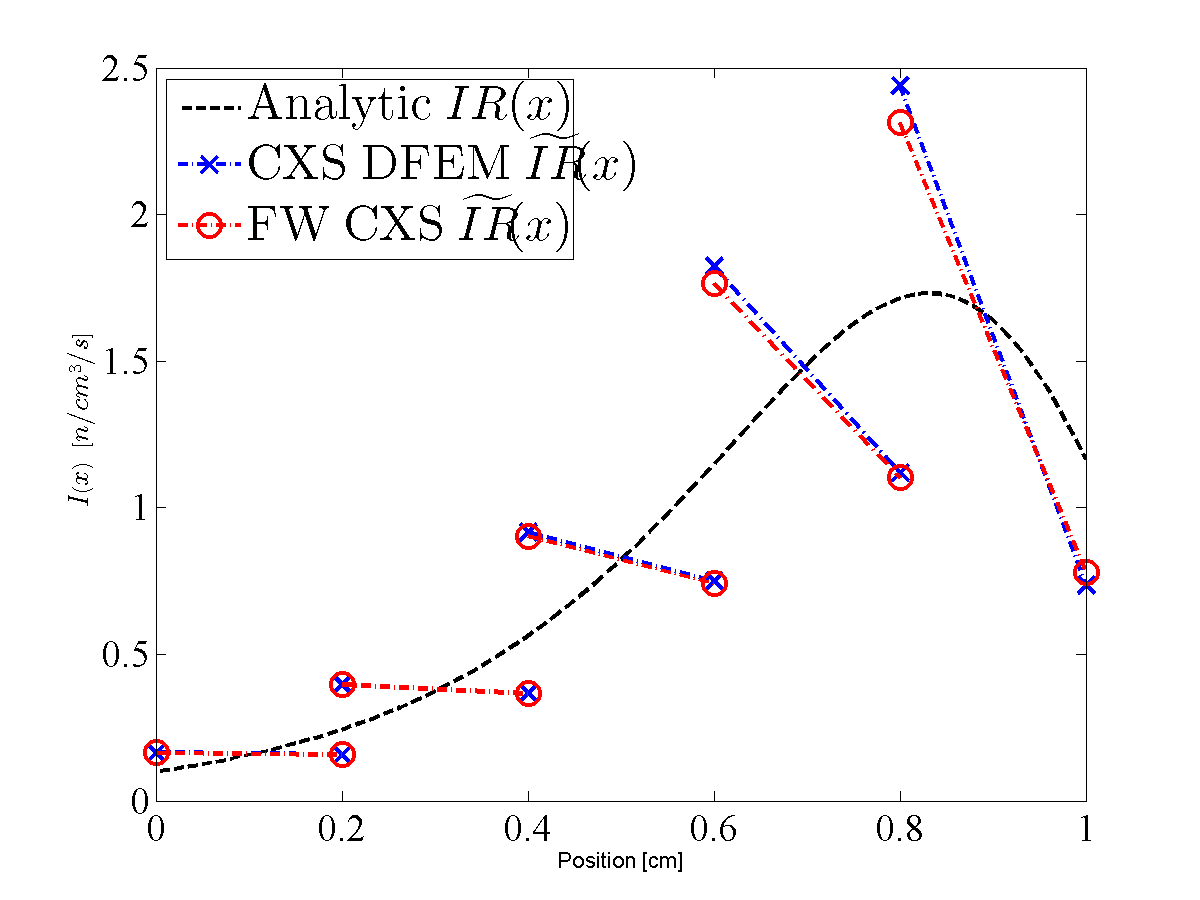
\includegraphics[width=11cm]{chapter3_variable_xs/FW_I_Blades.png}
}
\end{center}
\caption{Plot of the linear trial space FW CXS and CXS DFEM approximations $\widetilde{\psi}(x)$ and $\widetilde{IR}(x)$ for the pure absorber problem.}
\label{fig:fw_blading}
\end{figure}

%%%%%%%%%%%%%%%%%%%%%%%%%%%%%%%%

%%%%%%%%%%%%%%%%%%%%%%%%%%%%%%%%

\subsection{Effects of Mesh Spacing}
%%%%%%%%%%%%%%%%%%%%%%%%%%%%%%%%

In practice, computational domains are not necessarily discretized with uniform grids; rather cells are concentrated in regions where the solution is known or assumed to vary rapidly.  
For the pure absorber problem, we compare two alternative methods of mesh spacing (logarithmic grids and equal optical thickness grids, see \tbl{tbl:spacing_labels}),
to the results obtained with equally-spaced mesh cells.
We derive how to generate these meshes in \secref{sec:mesh_gen} and give results in \secref{sec:mesh_results}
\subsubsection{Generating Improved Spatial Meshes}  

Two alternative meshing strategies are compared to equally-spaced meshed.
In the following, we will use a shorthand notation, given in \tbl{tbl:spacing_labels}.
With the MFP meshing strategy, we find each cell width by determining the width of each cell from $i=1$ (leftmost cell) to $i=N_{cell}$ as outlined by \eqt{eq:chap3_mfp_spacing}:
\begin{subequations}
First, we determine the average cell optical thickness:
\label{eq:chap3_mfp_spacing}
\benum
\bar{h} = \frac{  \int_{x_{1/2}}^{x_{N_{cell}+1/2}}{ \Sigma_t(x)~dx} }{ N_{cell} } \pep
\eenum
Then, we solve the following equation for $x_{i+1/2}$:
\benum
\int_{x_{i-1/2}}^{x_{i+1/2}}{\Sigma_t(x)~dx} - \bar{h}  = 0 \pec
\eenum
yielding
\benum
x_{i+1/2} = \frac{1}{c_2} \log\left[ \frac{c_2( \bar{h} + \Sigma_t(x_{i-1/2}) }{c_1} \right] \pep
\eenum
\end{subequations}
%PSI spacing requires a priori knowledge of the analytic solution.  For the pure absorber problem, it is thus feasible to use PSI spacing, but in general PSI spacing would not be feasible.  Starting again from $i=1$, we find the width of each cell through the logic outlined in \eqt{eq:chap3_psi_spacing}
%\begin{subequations}
%\label{eq:chap3_psi_spacing}
%\beanum
%D &=& \frac{\psi(x_{N_{cell}+1/2},\mu_d) - \psi(x_{1/2},\mu_d) }{ N_{cell} } \\
%\psi(x_{i+1/2},\mu_d) &=& \psi(x_{i-1/2},\mu_d) + D \\
%x_{i+1/2} &=& \frac{1}{c_2} \log\left[ \frac{c_2}{c_1} \left( \log \left(\psi_{in}(\mu_d) \right) - \log(\psi(x_{i+1/2},\mu_d)) + \frac{c_1}{c_2} \right) \right] \pep
%\eeanum
%\end{subequations}

There are several ways to specify LOG spacing, but we elected to set a ratio, $0.6$, between adjacent cell sizes with the caveat that we would set a minimum cell size, $\Delta x_{min}$.
In our convergence testing, at the first refinement when $\Delta x_{N_cell} < \Delta x_{min}$, the grid is ``fixed'' and all further refinements uniformly refine the ''fixed'' grid.  $\Delta x_{N_{cell}}$ is the cell width for the right most cell where, for $R < 1$,
\benum
\Delta x_i =\Delta x_1 R^{i-1}, ~i\in[1,N_{cell}] \pep
\eenum
$\Delta x_1$ is determined by requiring that the geometric series of cell widths completely fill the space:
\benum
\Delta x_1 = \left( x_{N_{cell}+1/2} - x_{1/2} \right) \frac{1-R}{1-R^{N_{cell} }}
\eenum
The grid is ``fixed'' by resetting the width of every cell whose width, if set to the value required for a purely logarithmically spaced grid with $R$ would be below  $\Delta x_{min}$, to $\Delta x_{min}$. 
After imposing this, cell widths are determined by requiring the cells that were not reset to fill the problem space logarithmically using $R$.
If there is no minimum cell width, at high mesh refinements, most cells will be infinitesimally small and the large cells will never be refined, causing error to stagnate. 
Logarithmic spacing represents the ``smart'' meshing strategy most likely to be employed in engineering practice as it requires the least amount of solution information prior to problem execution.  
For all of our calculations, we set $R=0.6$ and $\Delta x_{min} = 10^{-3}~[cm]$.

First, we note that the choice of mesh spacing method does not alter asymptotic convergence rates, as shown in \fig{fig:lobatto_spacing}.  Figure \ref{fig:lobatto_spacing} shows that the SLXS Lobatto scheme with a quadratic trial space converges $E_{\psi}$, $E_{\psi_A}$, $E_{IR}$, and $E_{IR_A}$ at the same asymptotic rate, regardless of grid spacing choice.  Plots showing other trial space degrees and DFEM schemes are omitted for brevity.  We also omit showing the convergence of $E_{\psi_{out}}$ as we have already demonstrated that the convergence rate of $E_{\psi_{out}}$ and $E_{IR_A}$are related and identical.
\begin{figure}[!htp]
\begin{center}
\subfigure[$E_{\psi}$]{
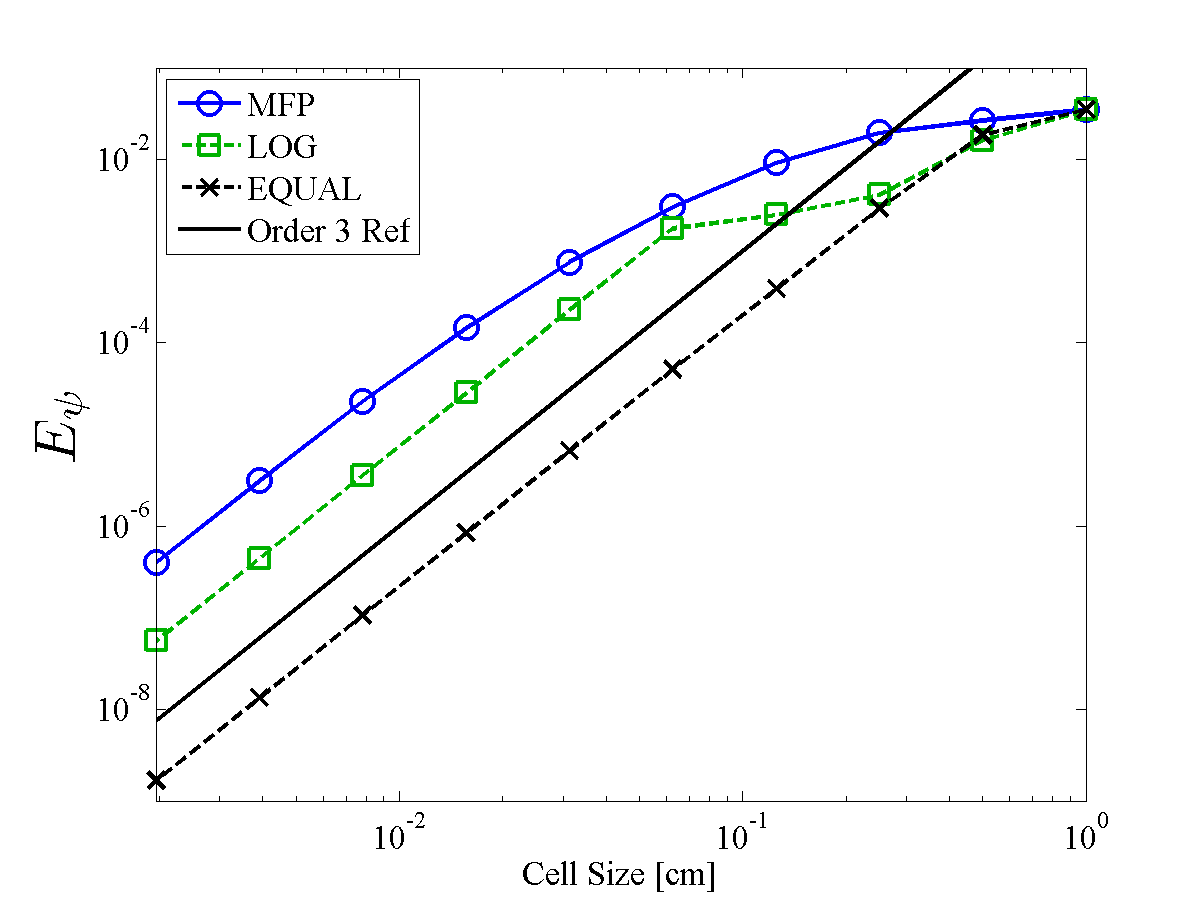
\includegraphics[width=11cm]{chapter3_variable_xs/P2_LOBATTO_E_PSI.png}
}
\subfigure[$E_{\psi_A}$]{
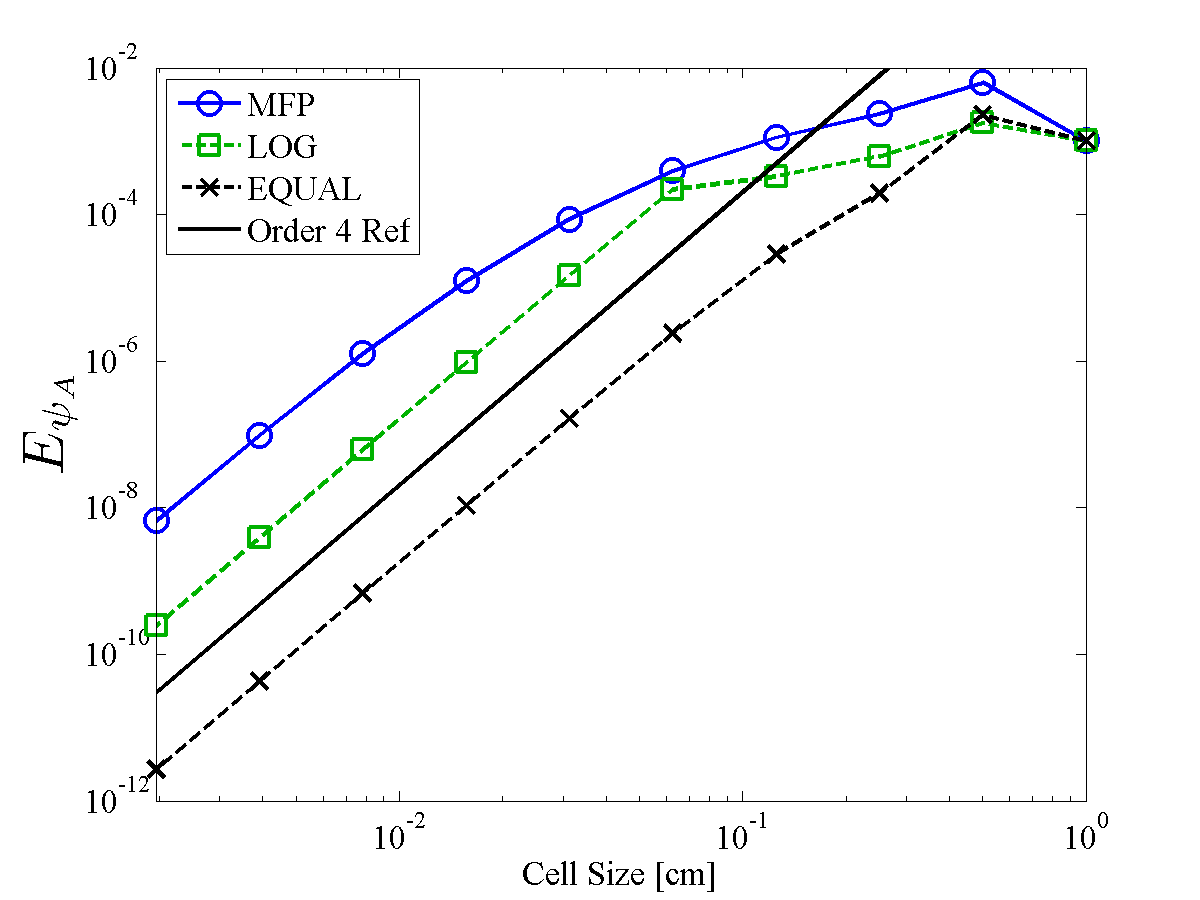
\includegraphics[width=11cm]{chapter3_variable_xs/P2_LOBATTO_E_PSI_A.png}
}
\subfigure[$E_{IR}$]{
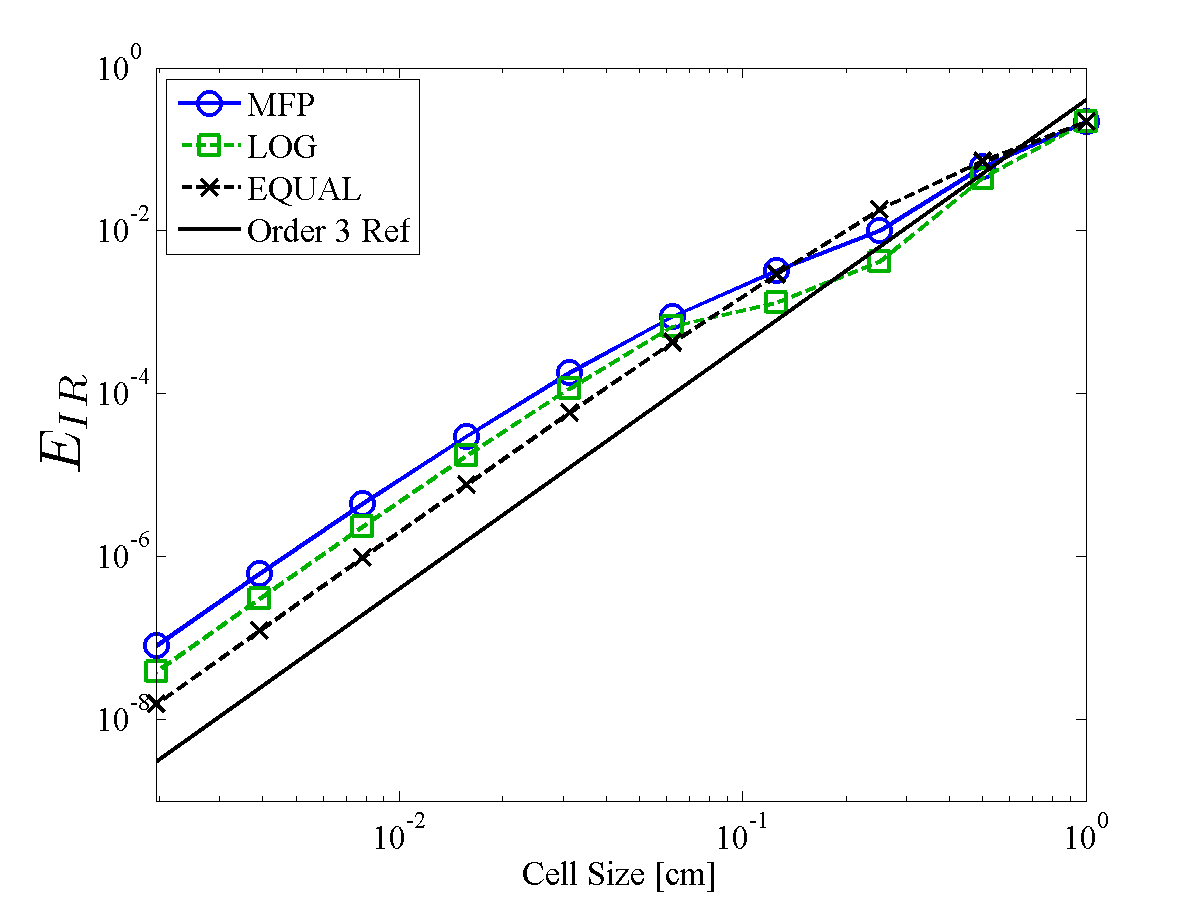
\includegraphics[width=11cm]{chapter3_variable_xs/P2_LOBATTO_E_IR.png}
}
\subfigure[$E_{IR_A}$]{
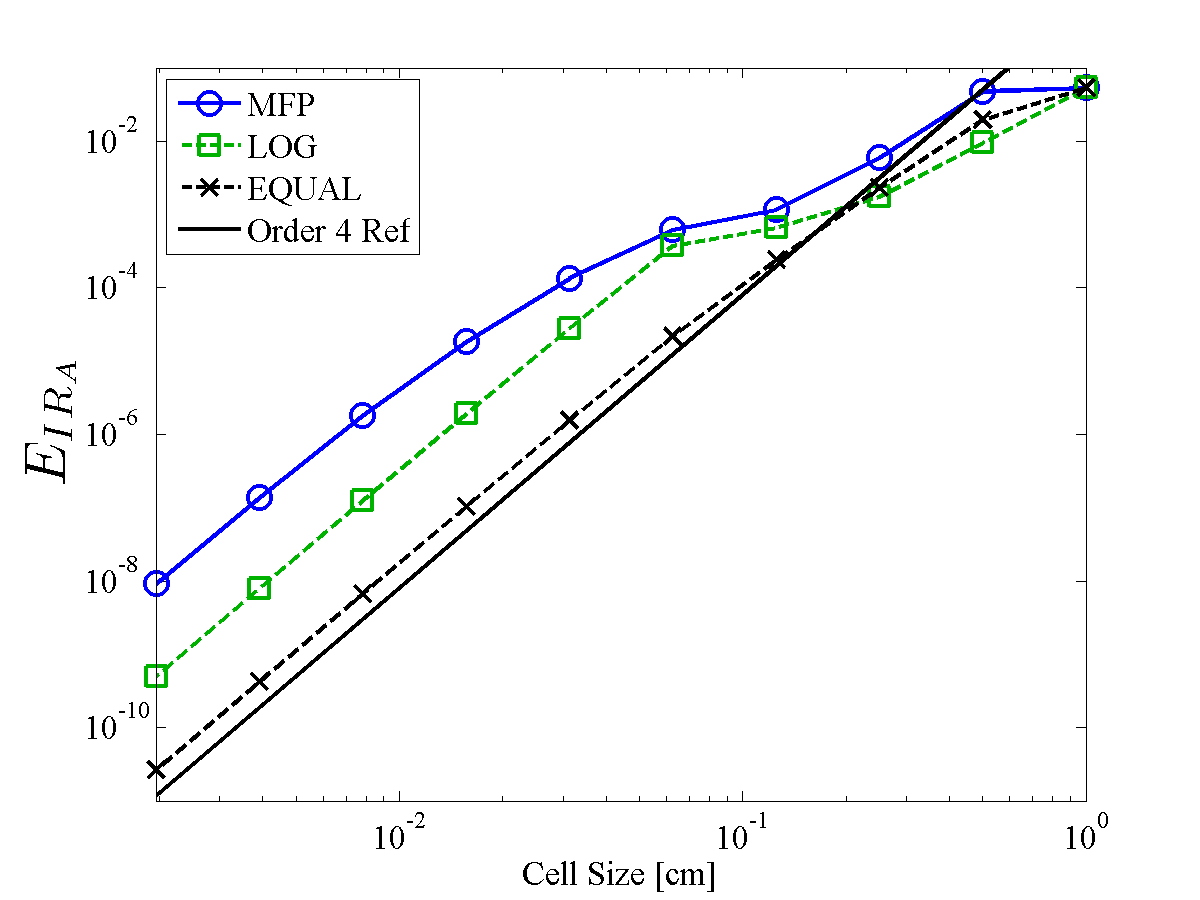
\includegraphics[width=11cm]{chapter3_variable_xs/P2_LOBATTO_E_IR_A.png}
}
\end{center}
\caption{Asymptotic convergence of the SLXS Lobatto scheme using a quadratic trial space, for different mesh spacing methodologies.}
\label{fig:lobatto_spacing}
\end{figure}
At mesh refinements that are not in the asymptotic convergence regime, the selection of a smart meshing methodology can result in a significant reduction in error.  
Consider \fig{fig:low_res_lobatto}, \fig{fig:low_res_gauss}, and \fig{fig:low_res_cxs} that show the values of $E_{\psi}$, $E_{\psi_A}$, $E_{IR}$, and $E_{IR_A}$ for the SLXS Lobatto, SLXS Gauss, and CXS DFEM schemes respectively for a quadratic trial space.
\begin{figure}[!htp]
\begin{center}
\subfigure[$E_{\psi}$]{
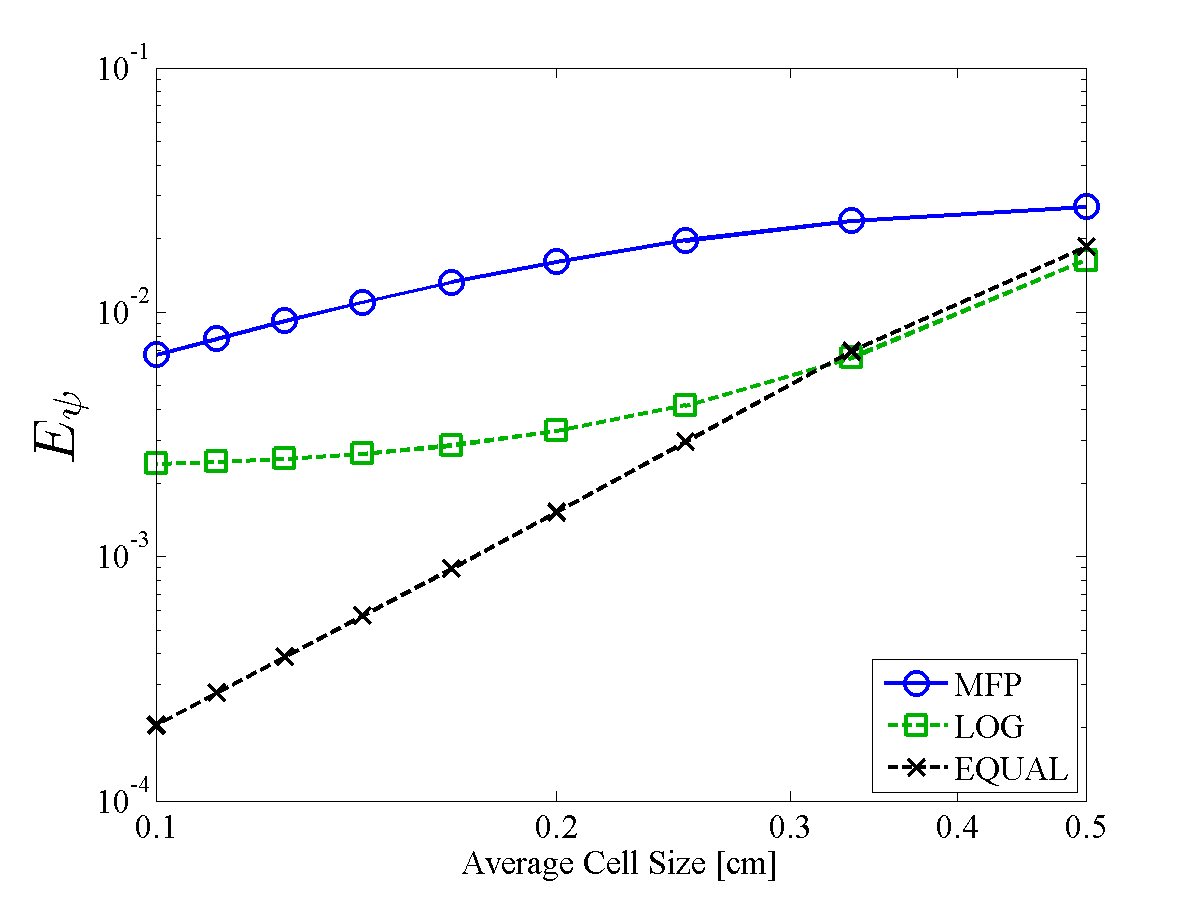
\includegraphics[width=11cm]{chapter3_variable_xs/LOW_RES_P2_LOBATTO_E_PSI.png}
}
\subfigure[$E_{\psi_A}$]{
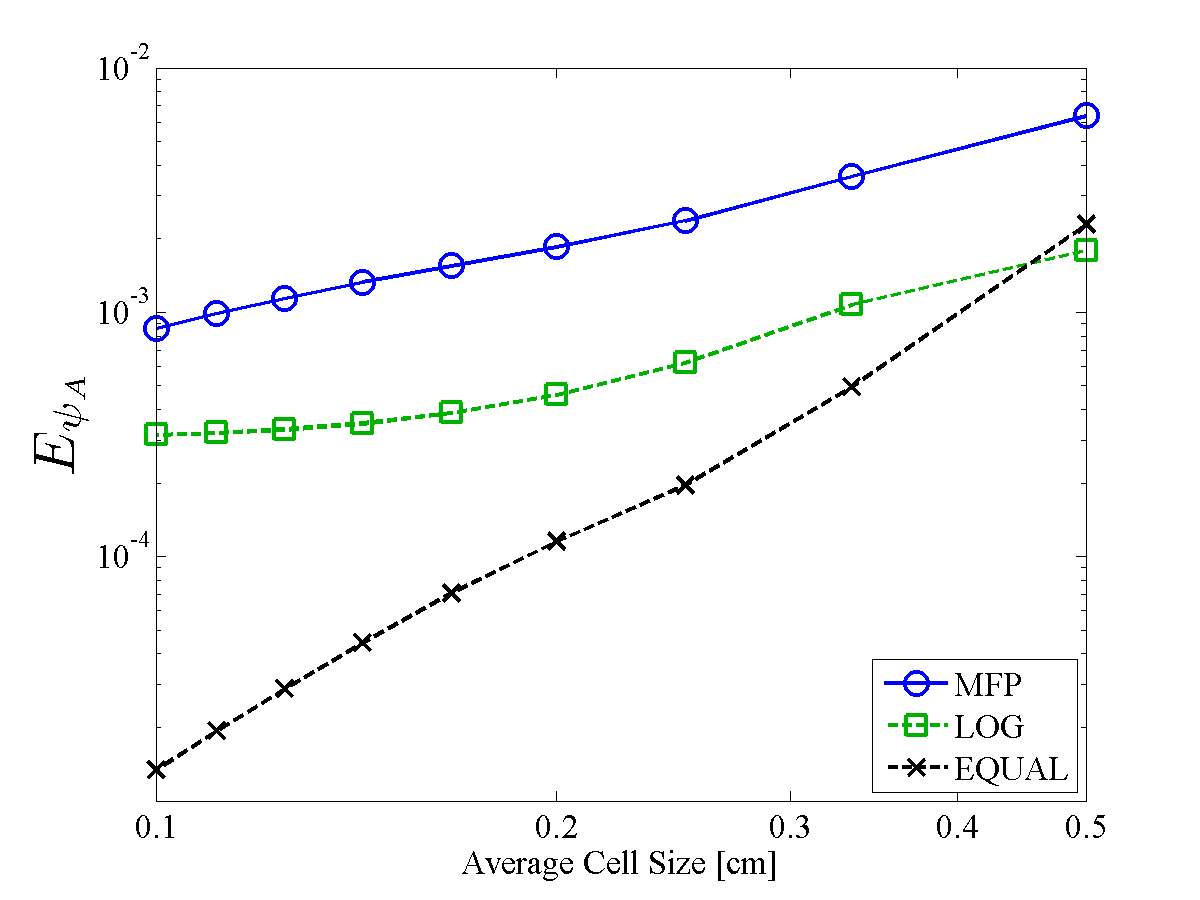
\includegraphics[width=11cm]{chapter3_variable_xs/LOW_RES_P2_LOBATTO_E_PSI_A.png}
}
\subfigure[$E_{IR}$]{
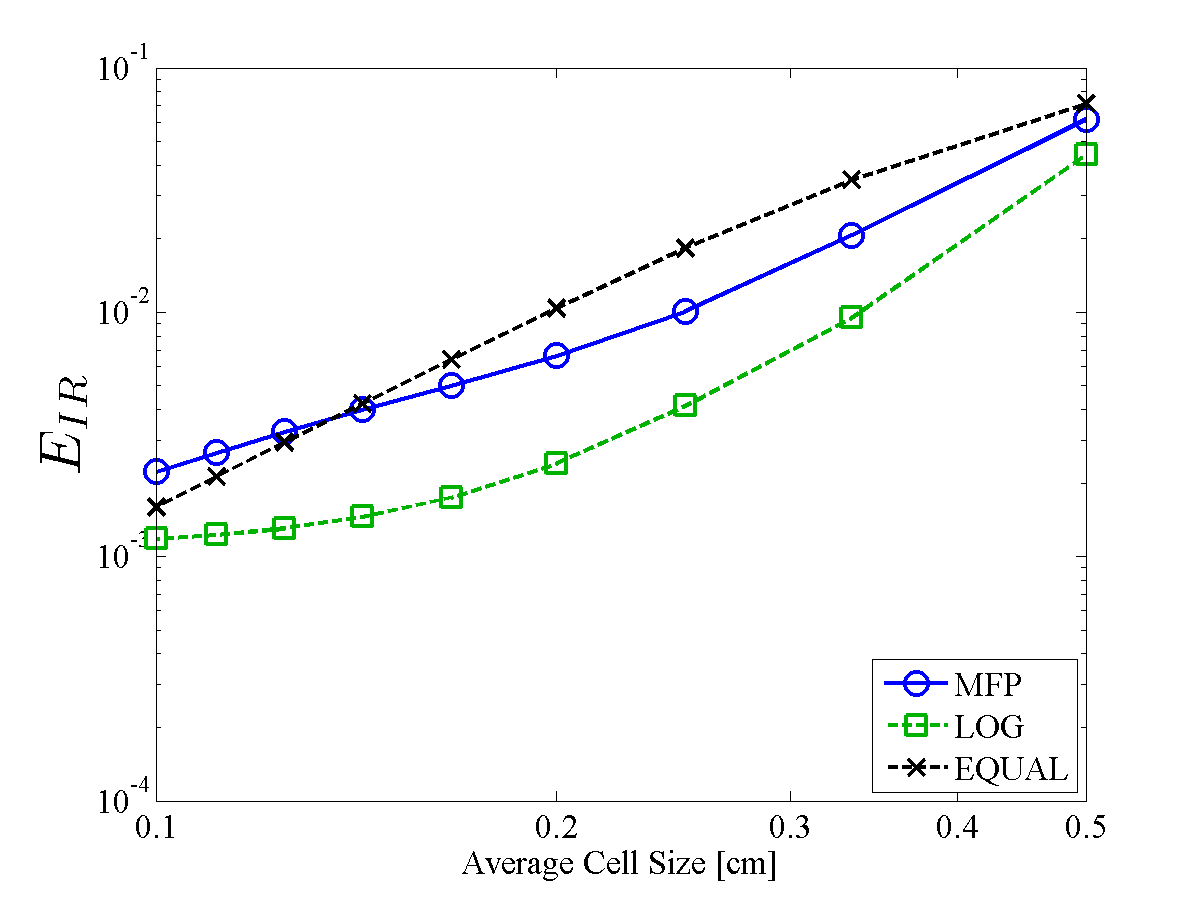
\includegraphics[width=11cm]{chapter3_variable_xs/LOW_RES_P2_LOBATTO_E_IR.png}
}
\subfigure[$E_{IR_A}$]{
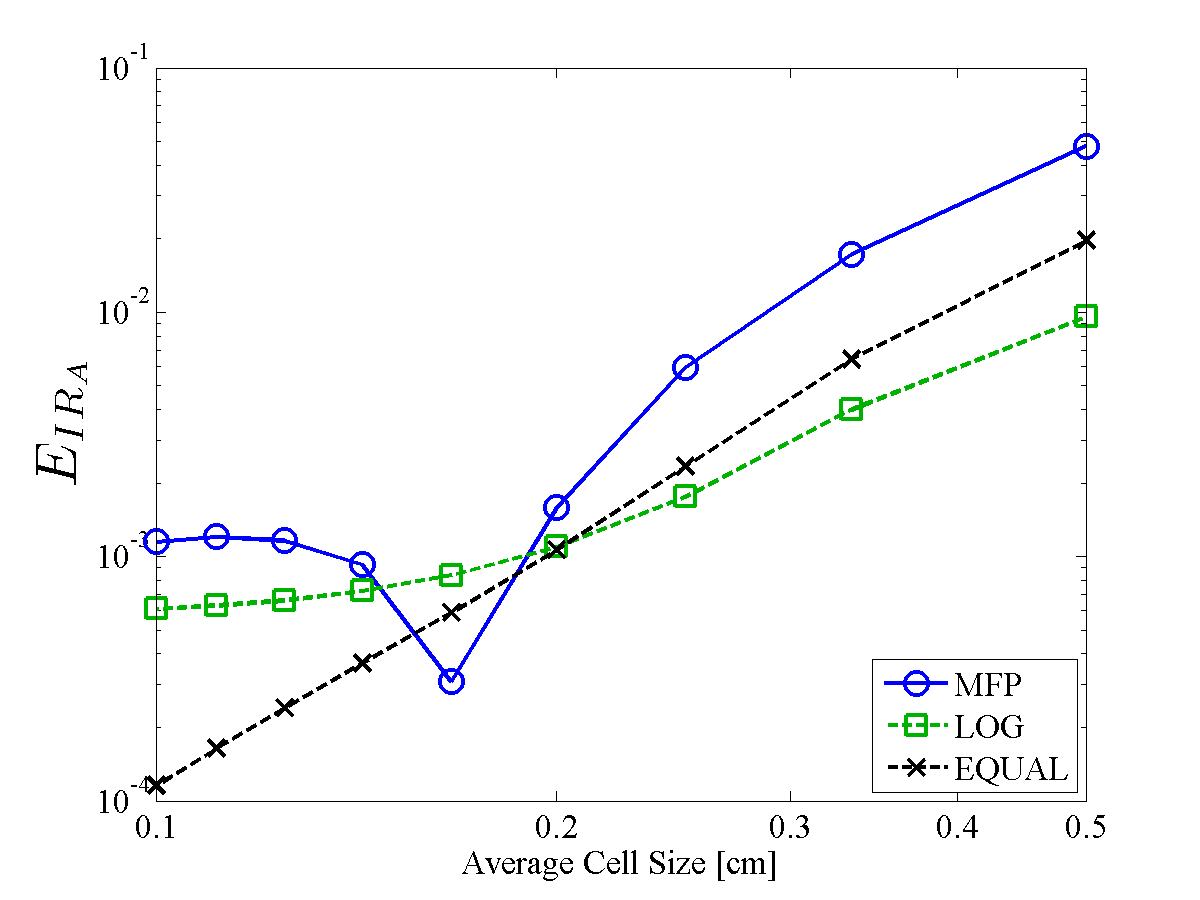
\includegraphics[width=11cm]{chapter3_variable_xs/LOW_RES_P2_LOBATTO_E_IR_A.png}
}
\end{center}
\caption{Errors associated with the SLXS Lobatto using a quadratic trial space scheme for different mesh spacing methodologies, at low resolutions.}
\label{fig:low_res_lobatto}
\end{figure}
%
%
\begin{figure}[!htp]
\begin{center}
\subfigure[$E_{\psi}$]{
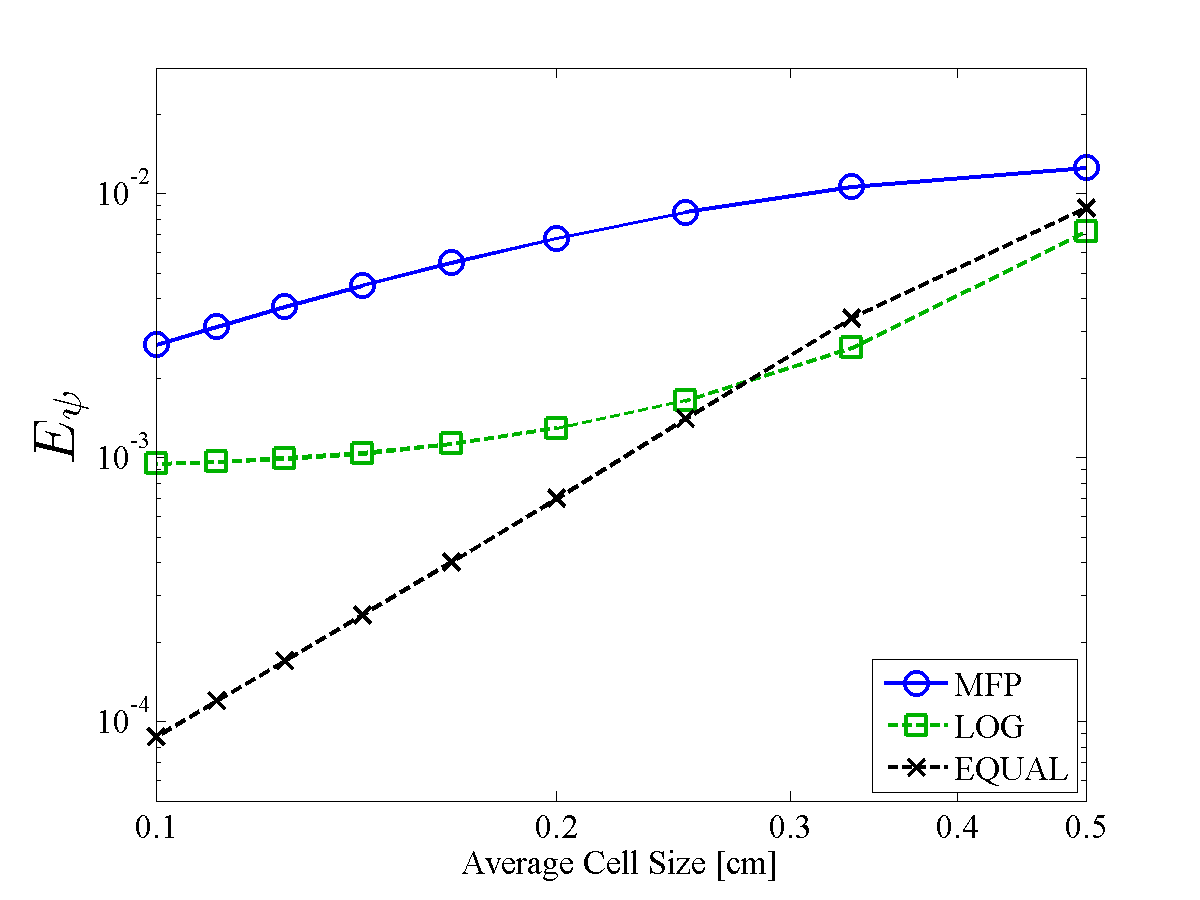
\includegraphics[width=11cm]{chapter3_variable_xs/LOW_RES_P2_GAUSS_E_PSI.png}
}
\subfigure[$E_{\psi_A}$]{
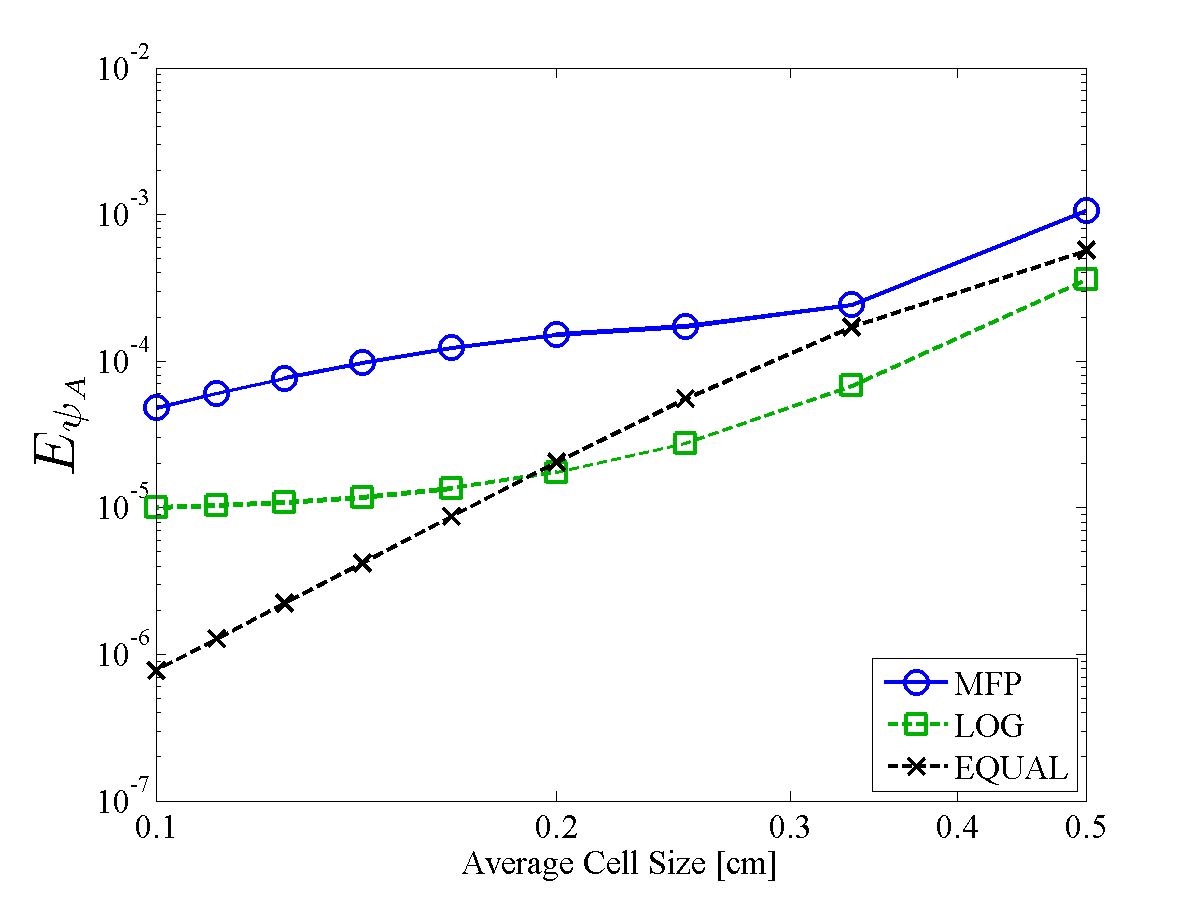
\includegraphics[width=11cm]{chapter3_variable_xs/LOW_RES_P2_GAUSS_E_PSI_A.png}
}
\subfigure[$E_{IR}$]{
\includegraphics[width=11cm]{chapter3_variable_xs/LOW_RES_P2_GAUSS_E_IR.png}
}
\subfigure[$E_{IR_A}$]{
\includegraphics[width=11cm]{chapter3_variable_xs/LOW_RES_P2_GAUSS_E_IR_A.png}
}
\end{center}
\caption{Errors associated with the SLXS Gauss using a quadratic trial space for different mesh spacing methodologies, at low resolutions.}
\label{fig:low_res_gauss}
\end{figure}
%
%
\begin{figure}[!htp]
\begin{center}
\subfigure[$E_{\psi}$]{
\includegraphics[width=11cm]{chapter3_variable_xs/LOW_RES_P2_CXS_E_PSI.png}
}
\subfigure[$E_{\psi_A}$]{
\includegraphics[width=11cm]{chapter3_variable_xs/LOW_RES_P2_CXS_E_PSI_A.png}
}
\subfigure[$E_{IR}$]{
\includegraphics[width=11cm]{chapter3_variable_xs/LOW_RES_P2_CXS_E_IR.png}
}
\subfigure[$E_{IR_A}$]{
\includegraphics[width=11cm]{chapter3_variable_xs/LOW_RES_P2_CXS_E_IR_A.png}
}
\end{center}
\caption{Errors associated with CXS DFEM using a quadratic trial space  for different mesh spacing methodologies, at low resolutions.}
\label{fig:low_res_cxs}
\end{figure}
First, we note that any particular mesh spacing methodology results in solutions that are more accurate for certain quantities, but not for all quantities.  
For example, with the self-lumping schemes, $E_{\psi}$ is generally smaller when using an equally spaced mesh, but using the LOG mesh results in orders of magnitude improvement in $E_{IR}$ and $E_{IR_A}$ on coarse meshes.
In \fig{fig:low_res_cxs}, CXS DFEM again illustrates that LOG spacing is more accurate in calculating interaction rate quantities than an equally-spaced mesh and equally-spaced meshes are generally more accurate than other meshing strategies for calculating angular flux quantities.
However, CXS DFEM shows a two order of magnitude reduction in calculating $E_{IR_A}$ when using a mesh that has a uniform optical thickness in each cell.  This is a direct result of CXS DFEM converging as $\hat{\sigma} \Delta x \to 0$.
%We conclude our discussion of mesh spacing by noting that LOG spacing was nearly as accurate at PSI spacing, without the requirement of knowing the solution prior to problem execution.


\subsubsection{Mesh Spacing Results}
\label{sec:mesh_results}
The important results from Figs. \ref{fig:lobatto_spacing}-\ref{fig:low_res_cxs} are summarized here:
\begin{enumerate}
\item mesh spacing does not affect asymptotic order of convergence,
\item accuracy in calculating certain quantities of interest (point-wise and cell averaged reaction rates) is improved with alternative meshing strategies at low resolution.
%\item accuracy in calculating the angular flux, is sacrificed.
\end{enumerate}
